%%%%%%%%%%%%%%%%%%%%%%%%%%%%%%%%%%%%%%%%%%%%%%%%%%%%%%%%%%%%%%%%%%%%%%%%%%%%%%%%
% Template for USENIX papers.
%
% History:
%
% - TEMPLATE for Usenix papers, specifically to meet requirements of
%   USENIX '05. originally a template for producing IEEE-format
%   articles using LaTeX. written by Matthew Ward, CS Department,
%   Worcester Polytechnic Institute. adapted by David Beazley for his
%   excellent SWIG paper in Proceedings, Tcl 96. turned into a
%   smartass generic template by De Clarke, with thanks to both the
%   above pioneers. Use at your own risk. Complaints to /dev/null.
%   Make it two column with no page numbering, default is 10 point.
%
% - Munged by Fred Douglis <douglis@research.att.com> 10/97 to
%   separate the .sty file from the LaTeX source template, so that
%   people can more easily include the .sty file into an existing
%   document. Also changed to more closely follow the style guidelines
%   as represented by the Word sample file.
%
% - Note that since 2010, USENIX does not require endnotes. If you
%   want foot of page notes, don't include the endnotes package in the
%   usepackage command, below.
% - This version uses the latex2e styles, not the very ancient 2.09
%   stuff.
%
% - Updated July 2018: Text block size changed from 6.5" to 7"
%
% - Updated Dec 2018 for ATC'19:
%
%   * Revised text to pass HotCRP's auto-formatting check, with
%     hotcrp.settings.submission_form.body_font_size=10pt, and
%     hotcrp.settings.submission_form.line_height=12pt
%
%   * Switched from \endnote-s to \footnote-s to match Usenix's policy.
%
%   * \section* => \begin{abstract} ... \end{abstract}
%
%   * Make template self-contained in terms of bibtex entires, to allow
%     this file to be compiled. (And changing refs style to 'plain'.)
%
%   * Make template self-contained in terms of figures, to
%     allow this file to be compiled.
%
%   * Added packages for hyperref, embedding fonts, and improving
%     appearance.
%
%   * Removed outdated text.
%
%%%%%%%%%%%%%%%%%%%%%%%%%%%%%%%%%%%%%%%%%%%%%%%%%%%%%%%%%%%%%%%%%%%%%%%%%%%%%%%%

\documentclass[letterpaper,twocolumn,10pt]{article}
\usepackage{usenix-2020-09}

% to be able to draw some self-contained figs
\usepackage{tikz}
\usepackage{amsmath}

\usepackage{filecontents}
\usepackage{graphicx}
\usepackage{amsthm}
\usepackage{amssymb}
\usepackage{thmtools}
\usepackage{color}
\usepackage{enumitem}
\usepackage{bm}

\usepackage[linesnumbered, lined, boxed]{algorithm2e}

\usepackage[normalem]{ulem}

\newtheorem{definition}{Definition}
\newtheorem{theorem}{Theorem}
\newtheorem{lemma}{Lemma}
\newtheorem{proposition}{Proposition}
\newtheorem{corollary}{Corollary}
\newtheorem{remark}{Remark}

\SetKwInput{KwData}{Input}
\SetKwInput{KwResult}{Output}

\newcommand{\MSE}{\operatorname{\textsf{MSE}}}

% \def\AlgWS{\textsf{WShuffle}$_{i,j}$}
\def\AlgWS{\textsf{WS}}
\def\AlgWSLE{\textsf{WSLE}}
\def\AlgWSTri{\textsf{WShuffle}$_{\triangle}$}
% \def\AlgWSTri{\textsf{WSLE}$_{\triangle}$}
\def\AlgWSTriVR{\textsf{WShuffle}$_{\triangle}^*$}
% \def\AlgWSTriVR{\textsf{WSLE}$_{\triangle}^*$}

\def\AlgWLTri{\textsf{WLocal}$_{\triangle}$}
\def\AlgARRTri{\textsf{ARR}$_{\triangle}$}
\def\AlgRRTri{\textsf{RR}$_{\triangle}$}
\def\AlgTwoRL{\textsf{2R-Large}$_{\triangle}$}
\def\AlgTwoRS{\textsf{2R-Small}$_{\triangle}$}

\def\AlgWSCyc{\textsf{WShuffle}$_{\square}$}
\def\AlgWLCyc{\textsf{WLocal}$_{\square}$}



\usepackage{hyperref}
\newcommand{\footremember}[2]{%
    \thanks{#2}
    \newcounter{#1}
    \setcounter{#1}{\value{footnote}}%
}
\newcommand{\footrecall}[1]{%
    \footnotemark[\value{#1}]%
}

\hypersetup{
  colorlinks,
  linkcolor={black},
  citecolor={red!70!black},
  urlcolor={blue!70!black}
}

% Switch conference/arXiv versions
%\newif\ifconferenceon\conferenceonfalse
\newif\ifconferenceon\conferenceontrue
\ifconferenceon
\newcommand{\conference}[1]{#1}
\newcommand{\arxiv}[1]{}
\else
\newcommand{\conference}[1]{}
\newcommand{\arxiv}[1]{#1}
\usepackage{balance}
\fi

\pagestyle{empty}

%-------------------------------------------------------------------------------
\begin{document}
%-------------------------------------------------------------------------------

% %don't want date printed
% \date{}

% make title bold and 14 pt font (Latex default is non-bold, 16 pt)
\title{\Large \bf Communication-Efficient Triangle Counting under Local Differential Privacy}
% \thanks{This study was supported in part by JSPS KAKENHI JP19H04113.}}

\author{
{\rm Jacob Imola}\footremember{contributions}{The first and second authors made equal contribution.}\\
UC San Diego
\and
{\rm Takao Murakami}\footrecall{contributions}\\
AIST
\and
{\rm Kamalika Chaudhuri}\\
UC San Diego
} % end author

\maketitle

%-------------------------------------------------------------------------------
\begin{abstract}
%-------------------------------------------------------------------------------

Triangle counting in networks under LDP (Local Differential Privacy) is a fundamental task for analyzing connection patterns or calculating a 
clustering coefficient while strongly protecting sensitive friendships from a central server. In particular, a recent study proposes an algorithm
for this task that uses two rounds of interaction between users and the server to significantly reduce estimation error. However,
this algorithm suffers from a prohibitively 
% large 
high 
communication cost due to a large noisy graph each user needs to download.

% In this work, we propose triangle counting algorithms under LDP with a small estimation error and small communication cost. This is achieved by
% two algorithmic techniques -- an asymmetric version of randomized response, coupled with selective edge sampling and a double-clipping technique. 
% Through comprehensive evaluations, we show that our algorithms reduce the communication cost by a factor of more than 3600 while retaining the
% same estimation error. 

% Triangle counting in graphs under LDP (Local Differential Privacy) has been studied to analyze connection patterns or to calculate a clustering coefficient while strongly protecting sensitive friendships even from a central server.
% % Triangle counting in graph data is a fundamental task
% % A triangle count in graph data is one of the most basic subgraph counts useful, e.g., for calculating a clustering coefficient.
% % or constructing graph models.
% % To strongly protect sensitive friendship information even from a central server,
% % it is desirable to use
% % some studies adopt
% % LDP (Local Differential Privacy) as a privacy metric.
% % Some studies propose triangle counting algorithms under LDP (Local Differential Privacy) to
% % strongly protect sensitive friendship information even from a central server.
% In particular, a recent study shows that
% % the estimation error is significantly reduced by introducing an additional round between users and the server.
% although
% algorithms with one round of interaction between users and the server suffer from a very large estimation error,
% % and that
% the error is significantly reduced by introducing an additional round.
% % However, existing algorithms suffer from either a prohibitively large estimation error
% % due to a single round of interaction between users and the server
% % or prohibitively large communication cost
% % due to a large noisy graph each user needs to download at an additional round.
% % , hence unpractical for a large graph.
% % However,
% Their two-rounds algorithm however suffers from a prohibitively large communication cost
% due to a large noisy graph each user needs to download.
% % at the second round.
% % because each user needs to download a large noisy graph at the additional round.
% % Thus, they cannot be

In this work, we propose triangle counting algorithms under LDP with a small estimation error and communication cost.
We first
% show that simply sampling edges in the noisy graph results in a large estimation error
propose two-rounds algorithms
consisting of edge sampling and carefully selecting edges each user downloads
% that sample noisy edges and then carefully select noisy edges each user downloads
so that the estimation error is small.
Then we propose
a double clipping technique,
which clips the number of edges and then the number of noisy triangles,
% a combination of
% edge clipping and noisy triangle clipping,
% which we call double clipping,
to significantly reduce the sensitivity of each user's query.
Through comprehensive evaluation, we 
% We comprehensively evaluate our algorithms using two real datasets, and
% Our experimental results
show that our algorithms dramatically reduce the communication cost
% when compared with
of the existing algorithm, e.g., from
% 400 Gbits to 100 Mbits
6 hours to 8 seconds or less at a 20 Mbps download rate, while keeping
a small estimation error.
% the relative error much smaller than 1.
\end{abstract}

\section{Introduction}
\label{chap3-sec:intro}
Graph statistics is useful for finding meaningful connection patterns in network data, and 
% counting subgraphs (e.g., triangles, $k$-stars, cycles, cliques) 
subgraph counting is known as a fundamental task in graph analysis. 
For example, a triangle is a cycle of size three, 
% consists of three nodes with three edges, 
and a $k$-star consists of a central node connected to $k$ other nodes.  
These subgraphs 
% important because they 
can be used to calculate 
a 
% (global) 
clustering coefficient ($=\frac{3 \times \text{\#triangles}}{\text{\#2-stars}}$). 
In a social graph, the clustering coefficient measures 
the tendency of nodes (users) to form a cluster with each other. 
% the degree to which nodes (users) tend to cluster together 
It also represents the average probability that a friend's friend is also a friend \cite{Newman_PRL09}. 
% two friends of a user will also be a friend 
Therefore, the clustering coefficient is useful for analyzing the effectiveness of friend suggestions. 
% For another example, a 4-cycle is a cycle composed of four nodes 
Another example of the subgraph is a 4-cycle, 
% which is a cycle composed of four nodes. 
a cycle of size four. 
The 4-cycle count is useful for measuring the clustering ability in bipartite graphs (e.g., 
% sexual contact networks \cite{Lind_PRE05}) 
online dating networks, mentor-student networks \cite{Kutty_WWW14}) 
where a triangle never appears \cite{Lind_PRE05,Robins_CMOT04,Sanei-Mehri_CIKM19}. 
Figure~\ref{chap3-fig:subgraphs} shows examples of triangles, 2-stars, and 4-cycles. 
% 
% Although subgraph counts are important for analyzing the connection patterns or clustering tendency, they can leak sensitive edges (friendships). 
Although these subgraphs are important for analyzing the connection patterns or clustering tendencies, their exact numbers can leak sensitive edges (friendships) \cite{Imola_USENIX21}. 
%include sensitive data such as sensitive friendships. 
% For example, in Figure~XX, the triangle count 

\begin{figure}[t]
  \centering
  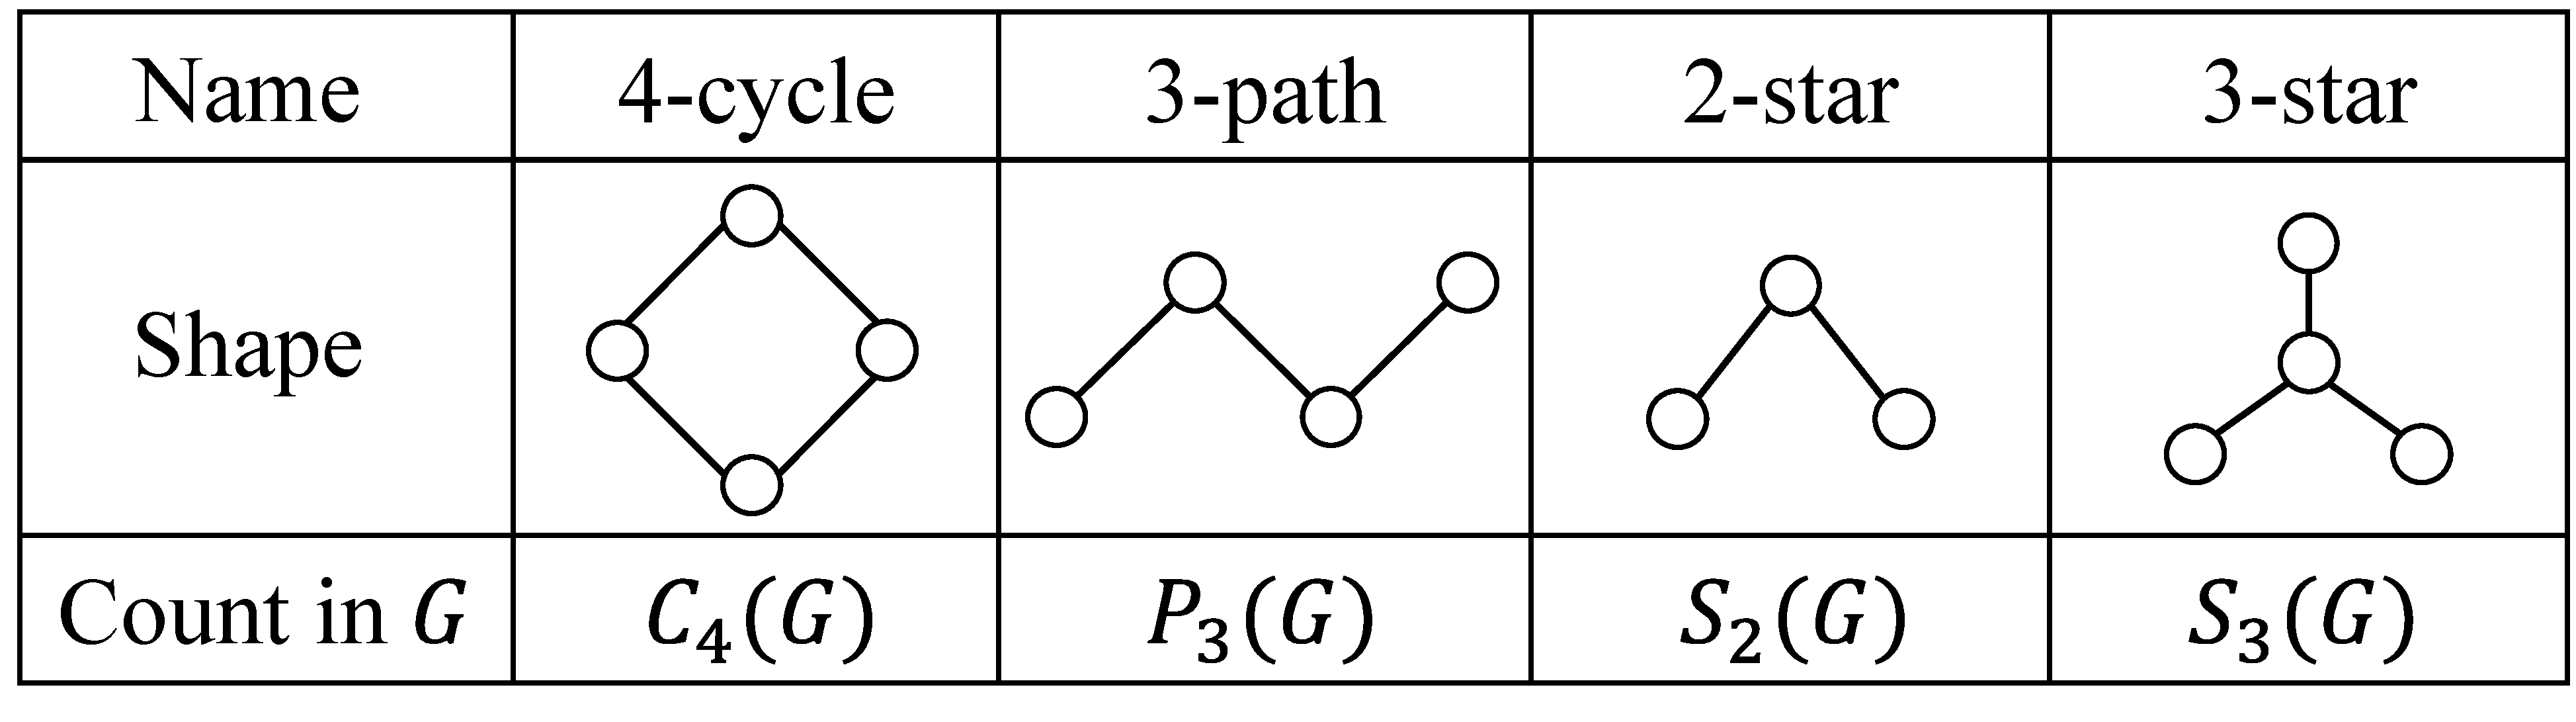
\includegraphics[width=0.65\linewidth]{fig/subgraphs.pdf}
  
  \caption[Examples of subgraph counts.]{Examples of subgraph counts.
  }
  \label{chap3-fig:subgraphs}
\end{figure}

DP (Differential Privacy) \cite{Dwork_ICALP06,DP} -- the gold standard of privacy notions -- has been widely used to strongly protect edges in graph data \cite{Day_SIGMOD16,Ding_TKDE21,Hay_ICDM09,Imola_USENIX21,Imola_USENIX22,Karwa_PVLDB11,Kasiviswanathan_TCC13,qin2017generating,Sun_CCS19,Ye_ICDE20,Ye_TKDE21}. 
% DP strongly protects user privacy when a parameter (privacy budget) $\epsilon$ is small and is known as the gold standard of privacy notions. 
% against adversaries with any background knowledge. 
In particular, recent studies 
\cite{Imola_USENIX21,Imola_USENIX22,qin2017generating,Ye_ICDE20,Ye_TKDE21} 
% \cite{Imola_USENIX21,Imola_USENIX22,Ye_ICDE20,Ye_TKDE21} 
have applied LDP (Local DP) \cite{Kasiviswanathan_FOCS08} to 
graph data. 
% subgraph counting. 
% where each user has 
%subgraph counting. 
In the graph LDP model, each user obfuscates her neighbor list (friends list) by herself and sends the obfuscated neighbor list to a data collector. 
Then, the data collector estimates graph statistics, such as subgraph counts. 
Compared to central DP where a central server has personal data of all users (i.e., the entire graph), LDP does not have a risk that all personal data are leaked from the server by 
% illegal access 
cyberattacks 
\cite{Henriquez_breach2021} or insider attacks \cite{Kohen_insider_threats}. 
Moreover, LDP can be applied to decentralized social networks \cite{Paul_CN14,Salve_CSR18} (e.g., diaspora* \cite{Diaspora}, Mastodon \cite{Mastodon}) where no server can access the entire graph; e.g., 
the entire graph is distributed across many servers, or no server has any original edges. 
It is reported in \cite{Imola_USENIX21} that $k$-star counts can be accurately estimated in this model. 

However, it is much more challenging to accurately count more complicated subgraphs such as triangles and 4-cycles under LDP. 
The root cause of this is its local property -- a user cannot see edges between others. 
% For example, user $v_3$ knows that there are ten $2$-stars of which she is a center. 
% However, $v_3$ cannot count triangles or 4-cycles including $v_3$, as she cannot see edges between others, e.g., $(v_1,v_2)$ and $(v_2,v_4)$. 
For example, user $v_1$ cannot count triangles or 4-cycles including $v_1$, as she cannot see edges between others, e.g., $(v_2,v_3)$, $(v_2,v_4)$, and $(v_3,v_4)$. 
Therefore, the existing algorithms \cite{Imola_USENIX21,Imola_USENIX22,Ye_ICDE20,Ye_TKDE21} 
obfuscate 
each bit of the neighbor list 
% each user's edges 
rather than the subgraph count by 
% apply 
% Warner's 
the RR (Randomized Response) \cite{Warner_JASA65}, which randomly flips 0/1. 
% with some probability, 
% to each bit of the neighbor list. 
As a result, their algorithms suffer from extremely large estimation errors because it makes all edges noisy. 
% any triangle or 4-cycle. 
% To address this issue, 
Some studies \cite{Imola_USENIX21,Imola_USENIX22} 
significantly improve the accuracy by introducing 
% introduce 
an additional round of interaction between users and the data collector. 
% Their algorithms publish the noisy graph at the first round to enable each user to count her triangles such that only one edge is noisy at the second round. 
% In their algorithms, the data collector publishes the noisy graph at the first round. 
% Specifically, they propose triangle algorithms that publish the noisy graph at the first round 
% so that each user can count her triangles at the second round. 
% Then, at the second round, each user can count her triangles such that only one edge is noisy. 
% because she knows two edges connected to her. 
% Therefore, the accuracy is significantly improved. 
% Thus, the two-rounds algorithms significantly reduce the estimation error. 
However, multi-round interaction may be impractical in many applications, as it requires a lot of user effort and synchronization; 
in  \cite{Imola_USENIX21,Imola_USENIX22}, every user must respond twice, and the data collector must wait for responses from all users 
in each round. 
% to publish the noisy graph. 

In this work, we focus on a \textbf{one-round} of interaction between users and the data collector and propose accurate subgraph counting algorithms by introducing a recently studied privacy model: the \textit{shuffle model} \cite{Erlingsson_SODA19,Feldman_FOCS21}. 
% The shuffle model introduces an intermediate server called the shuffler. 
In the shuffle model, each user sends her (encrypted) obfuscated data to an intermediate server called the shuffler. 
Then, the shuffler randomly shuffles the obfuscated data of all users and sends the shuffled data to the data collector (who decrypts them). 
% It has been proven that 
The shuffling amplifies DP guarantees of the obfuscated data under the assumption that the shuffler and the data collector do not collude with each other. 
Specifically, it is known that DP strongly protects user privacy when a parameter (a.k.a. privacy budget) $\epsilon$ is small, e.g., $\epsilon \leq 1$ \cite{DP_Li}. 
The shuffling significantly reduces $\epsilon$ and therefore significantly improves utility at the same value of $\epsilon$. 
To date, the shuffle model has been successfully applied to tabular data \cite{Meehan_ICLR22,Wang_PVLDB20} and 
% image data 
gradients \cite{Girgis_AISTATS21,Liu_AAAI21} in federated learning. 
We 
%make the first attempt (to our knowledge) to apply the shuffle model to subgraph counting. 
apply the shuffle model to graph data to accurately count subgraphs within one round. 
%one-round subgraph counting to provide a small estimation error. 

% However, it is very challenging to apply the shuffle model to subgraph counting because 
The main challenge in subgraph counting in the shuffle model is that each user's neighbor list is \textit{high-dimensional data}, i.e., $n$-dim binary string where $n$ is the number of users. 
% we cannot use the entire neighbor list as input data. 
Consequently, applying the RR to each bit of the neighbor list, as in the existing work \cite{Imola_USENIX21,Imola_USENIX22,Ye_ICDE20,Ye_TKDE21}, results in an extremely large privacy budget $\epsilon$ even after applying the shuffling (see Section~\ref{chap3-sub:technical} for more details). 

We address this issue by introducing a new, basic technique called \textit{wedge shuffling}. 
In graphs, a wedge between $v_i$ and $v_j$ is defined by a 2-hop path with endpoints $v_i$ and $v_j$. 
% Our wedge shuffle technique obfuscates a wedge (2-hop path) between a specific user-pair. 
% rather than the entire neighbor list. 
For example, in Figure~\ref{chap3-fig:subgraphs}, 
there are two wedges between $v_2$ and $v_3$: $v_2$-$v_1$-$v_3$ and $v_2$-$v_4$-$v_3$. 
In other words, users $v_1$ and $v_4$ have a wedge between $v_2$ and $v_3$, whereas $v_5, \ldots, v_8$ do not. 
Each user obfuscates such wedge information by the RR, and the shuffler randomly shuffles them. 
Because the wedge information (i.e., whether there is a wedge between a specific user-pair) 
is \textit{one-dimensional binary data}, it can be sent with small noise and small $\epsilon$. 
In addition, the wedge is the main component of several subgraphs, such as triangles, 4-cycles, and 3-hop paths \cite{Sun_CCS19}. 
Since the wedge has little noise, we can accurately count these subgraphs based on wedge shuffling. 

We apply wedge shuffling to triangle and 4-cycle counting tasks with several additional techniques. 
For triangles, we first 
%consider a problem of counting 
propose an algorithm that counts triangles involving the user-pair at the endpoints of the wedges by locally sending an edge between the user-pair to the data collector. 
% along with shuffled wedges. 
% to count triangles including the user-pair. 
Then we propose an algorithm to count triangles in the entire graph by sampling disjoint user-pairs, which share no common users (i.e., 
no user falls in two pairs). 
We also propose a technique to reduce the variance of the estimate by ignoring sparse user-pairs, where either of the two users has a very small degree. 
For 4-cycles, we propose an algorithm to calculate an unbiased estimate of the 4-cycle count from that of the wedge count via bias correction. 

% We propose triangle and 4-cycle counting algorithms based on our wedge shuffle technique and show upper bounds on the estimation error for our algorithms. 
We provide upper bounds on the estimation error for our triangle and 4-cycles counting algorithms. 
Through comprehensive evaluation, we show that 
% it is possible to accurately estimate 
our algorithms 
accurately estimate these subgraph counts within one round under the shuffle model. 
% to triangles and 4-cycles. 
% with some additional techniques. 
% Our experimental results show that 

% \begin{itemize}
%     \item shuffle model for graphs?
%     \item define graph shuffle model
%     \item problem: high dim data
%     \item counting triangles/4-cycles
%     \item our approach: dim reduction by wedges
% \end{itemize}


\smallskip
\noindent{\textbf{Our Contributions.}}~~Our contributions are as follows: 
\begin{itemize}
    \item We propose a wedge shuffle technique to enable privacy amplification 
    %in subgraph counting. 
    of graph data. 
    To our knowledge, we are the first to shuffle graph data (see Section~\ref{chap3-sec:related} for more details). 
    %apply the shuffle model to graph data. 
    \item We propose one-round triangle and 4-cycle counting algorithms 
    %with theoretical performance guarantees 
    based on our wedge shuffle technique. 
    %apply wedge shuffling to triangles and 4-cycles. 
    For triangles, we propose three additional techniques: sending local edges, sampling disjoint user-pairs, and variance reduction by ignoring sparse user-pairs. 
    For 4-cycles, we propose a bias correction technique. 
    We show upper bounds on the estimation error for each algorithm. 
    \item We evaluate our algorithms using two real graph datasets. 
    Our experimental results show that our one-round shuffle algorithms 
    significantly outperform one-round local algorithms in terms of accuracy 
    %dramatically the estimation error of the one-round local algorithms 
    and achieve a small estimation error (relative error $\ll 1$) with a reasonable privacy budget, e.g., smaller than $1$ in edge DP. 
\end{itemize}
In \conference{the full version of this paper \cite{Imola_CCSFull22}}\arxiv{Appendix~\ref{chap3-sec:cluster}}, we show that our triangle algorithm is also useful for accurately estimating the clustering coefficient within one round. 
% we can also accurately estimate the clustering coefficient within one round by using our triangle algorithm. 
We can use our algorithms to analyze the clustering tendency or the effectiveness of friend suggestions in decentralized social networks by introducing a shuffler. 
We implemented our algorithms in C/C++. 
Our code is available on GitHub \cite{SubgraphShuffle}. 
The proofs of all statements in the main body are given in \conference{\cite{Imola_CCSFull22}}\arxiv{Appendices~\ref{chap3-sec:triangle_proof} and \ref{chap3-sec:4cycle_proof}}. 

\section{Related Work}
\label{sec:related}
% \smallskip
\noindent{\textbf{Non-private Subgraph Counting.}}~~Subgraph counting has been extensively studied in a non-private setting (see \cite{Ribeiro_CS21} for a recent survey). 
% Differentially priate graph analysis has been widely studied in the literature. 
% In particular, triangle counting is considered one of the most basic task 
Examples of subgraphs include triangles \cite{Bera_PODS20,Eden_FOCS15,Kolountzakis_IM12,Wu_TKDE16},  4-cycles \cite{Bera_STACS17,Kallaugher_PODS19,Manjunath_ESA11,McGregor_PODS20}, $k$-stars \cite{Aliakbarpour_Alg18,Gonen_DM11}, and 
$k$-hop paths \cite{Bjorklund_ICALP19,Kartun-Giles_TWC18}. 

Here, the main challenge is to reduce the computational time of counting these subgraphs in large-scale graph data. 
One of the simplest approaches is edge sampling \cite{Bera_PODS20,Eden_FOCS15,Wu_TKDE16}, which randomly 
% and independently 
samples edges in a graph. 
Edge sampling outperforms other sampling methods 
% approaches 
(e.g., node sampling, triangle sampling) \cite{Wu_TKDE16} and is also adopted in \cite{Imola_USENIX22} 
% to improve communication efficiency in 
for private triangle counting. 

Although our triangle algorithm also samples user-pairs, ours is different from edge sampling in two ways. 
First, our algorithm does not sample an edge but samples a pair of users who may or may not be a friend. 
% have an edge between them. 
Second, our algorithm samples user-pairs that share no common users to avoid the increase of the privacy budget $\epsilon$ as well as to reduce the time complexity 
(see Section~\ref{sec:triangle} for details). 

\smallskip
\noindent{\textbf{Private Subgraph Counting.}}~~Differentially private subgraph counting has been widely studied, and the previous work assumes either the central \cite{Ding_TKDE21,Karwa_PVLDB11,Kasiviswanathan_TCC13} or local \cite{Imola_USENIX21,Imola_USENIX22,Sun_CCS19,Ye_ICDE20,Ye_TKDE21} models. 
The central model assumes a centralized social network and has a data breach issue, as explained in Section~\ref{sec:intro}. 

Subgraph counting in the local model has recently attracted attention. 
Sun \textit{et al.} \cite{Sun_CCS19} propose subgraph counting algorithms 
% under the assumption 
assuming 
that each user knows all friends' friends. 
However, this assumption does not hold in many social networks; e.g., Facebook users can change their settings so that anyone cannot see their friend lists. 
Therefore, we make a minimal assumption -- each user knows only her friends. 

% Some studies \cite{Imola_USENIX21,Imola_USENIX22,Ye_ICDE20,Ye_TKDE21} focus on this setting. 

In this setting, recent studies propose triangle \cite{Imola_USENIX21,Imola_USENIX22,Ye_ICDE20,Ye_TKDE21} and $k$-star \cite{Imola_USENIX21} counting algorithms. 
% As described in Section~\ref{sec:intro}, 
For $k$-stars, Imola \textit{et al.} \cite{Imola_USENIX21} propose a one-round algorithm that is order optimal and show that it provides a very small estimation error. 
% Triangles are much more challenging than $k$-stars. 
% Ye \textit{et al.} \cite{Ye_ICDE20} propose a one-round algorithm that applies the RR to each bit of the neighbor list and then counts the number of triangles in the noisy graph. 
% They also propose an algorithm to reduce the bias in the estimate \cite{Ye_TKDE21} (though there is no proof that the estimate is unbiased). 
% Imola \textit{et al.} \cite{Imola_USENIX21} 
For triangles, they
propose a one-round algorithm that applies the RR to 
% bits for smaller user IDs in 
each bit of the neighbor list 
and then calculates an unbiased estimate of triangles from the noisy graph. 
We call this algorithm \AlgRRTri{}. 
Imola \textit{et al.} \cite{Imola_USENIX22} show that \AlgRRTri{} provides a much smaller estimation error than the one-round triangle algorithms in \cite{Ye_ICDE20,Ye_TKDE21}. 
In \cite{Imola_USENIX22}, they also reduce the time complexity of \AlgRRTri{} 
% from $O(n^3)$ to $O(n^2)$ 
by using the ARR (Asymmetric RR), which samples each 1 (edge) after applying the RR. 
We call this algorithm \AlgARRTri{}. 
In this paper, we use \AlgRRTri{} and \AlgARRTri{} as baselines in triangle counting. 
% compare our triangle algorithms with \AlgRRTri{} and \AlgARRTri{} in our theoretical analysis and with \AlgARRTri{} in our experiments (we cannot apply \AlgRRTri{} to large-scale graphs, as it is too inefficient; see ). 
For 4-cycles, there is no existing algorithm under LDP, to our knowledge. 
Thus, we compare our shuffle algorithm with its local version, which does not shuffle the obfuscated data. 

For triangles, Imola \textit{et al.} also propose a two-round local algorithm in \cite{Imola_USENIX21} and significantly reduce its download cost in \cite{Imola_USENIX22}. 
Although we focus on one-round algorithms, 
% as described in Section~\ref{sec:intro}. 
we show in 
% Section~\ref{sec:experiments} 
\conference{the full version \cite{Imola_CCSFull22}}\arxiv{Appendix~\ref{sec:two-round}} 
that our one-round algorithm is comparable to the two-round algorithm in \cite{Imola_USENIX22}, which requires a lot of user effort and synchronization, in terms of accuracy. 

% In this paper, we compare our triangle algorithms with \AlgRRTri{} and \AlgARRTri{} in our theoretical analysis and with \AlgARRTri{} in our experiments (we cannot apply \AlgRRTri{} to large-scale graphs, as it is too inefficient; see ). 

% one-round local triangle counting \cite{Imola_USENIX21,Imola_USENIX22,Ye_ICDE20,Ye_TKDE21}, \AlgARRTri{} \cite{Imola_USENIX22}, \AlgRRTri{} \cite{Imola_USENIX21}. Explain  and \AlgARRTri{} in detail because they are compared with our algorithms.

\smallskip
\noindent{\textbf{Shuffle Model.}}~~The privacy amplification by shuffling has been recently studied in \cite{Balle_CRYPTO19,Cheu_EUROCRYPT19,Erlingsson_SODA19,Feldman_FOCS21}. 
Among them, the privacy amplification bound by Feldman \textit{et al.} \cite{Feldman_FOCS21} is the state-of-the-art -- it provides a smaller $\epsilon$ than other bounds, such as \cite{Balle_CRYPTO19,Cheu_EUROCRYPT19,Erlingsson_SODA19}. 
%and is more general than the bound in \cite{Cheu_EUROCRYPT19} that is specific to binary RR. 
Girgis \textit{et al.} \cite{Girgis_CCS21} 
consider multiple interactions between users and the data collector and 
show a better bound than the bound in \cite{Feldman_FOCS21} when used with composition. 
However, the bound in \cite{Feldman_FOCS21} outperforms the bound in \cite{Girgis_CCS21} when used without composition. 
% (which is the case with this work that considers a single interaction). 
Because our work focuses on a single interaction and does not use the composition, 
% Therefore, 
we use the bound in \cite{Feldman_FOCS21}. 

The shuffle model has been applied to tabular data \cite{Meehan_ICLR22,Wang_PVLDB20} and gradients \cite{Girgis_AISTATS21,Liu_AAAI21} in federated learning. 
Meehan \textit{et al.} \cite{Meehan_ICLR22} construct a graph from public auxiliary information and determine a permutation of obfuscated data using the graph to reduce re-identification risks. 
Liew \textit{et al.} \cite{Liew_SIGMOD22} propose network shuffling, which shuffles obfuscated data via random walks on a graph. 
%, where users exchange their obfuscated data 
%each user relays her obfuscated data to her neighbor
Note that both \cite{Meehan_ICLR22} and \cite{Liew_SIGMOD22} use graph data to shuffle another type of data. 
% neither \cite{Meehan_ICLR22} or \cite{Liew_SIGMOD22} shuffles graph data itself (they shuffle another data using graph data). 
To our knowledge, our work is the first to shuffle graph data itself. 

 %-------------------------------------------------------------------------------
\section{Preliminaries}
%-------------------------------------------------------------------------------
\label{chap1-sec:preliminaries}

% \subsection{Notations and Graphs}
% \label{chap1-sub:notations}
% \subsection{Graphs and Centralized Differential Privacy}
\subsection{Graphs and Differential Privacy}
\label{chap1-sub:graphs_CDP}
\noindent{\textbf{Graphs.}}~~Let $\nats$, $\nnints$, $\reals$, and $\nnreals$ be the sets of natural numbers, non-negative integers, real numbers, and non-negative real numbers, respectively. 
For $a \in \nats$, let $[a] = \{1, 2, \ldots, a\}$. 

We consider an undirected graph $G=(V,E)$, where 
$V$ is a set of nodes (i.e., users) and $E$ is a set of edges. 
Let $n \in \nats$ be the number of users in $V$, and let $v_i \in V$ the $i$-th user; i.e., $V=\{v_1,\ldots,v_n\}$. 
An edge $(v_i, v_j) \in E$ represents a relationship between users $v_i \in V$ and $v_j \in V$. 
% a node $v \in V$ represents a user and an edge $(u,v) \in E$ represents a relationship
% between users $u \in V$ and $v \in V$. 
The number of edges connected to a single node is called the \textit{degree} of the node. 
Let $d_{max} \in \nats$ be the \textit{maximum degree} (i.e., maximum number of edges connected to a node) in graph $G$. 
Let $\calG$ be the set of possible graphs 
% $G=(V,E)$ with $V=\{v_1,\ldots,v_n\}$. 
$G$ on $n$ users. 
A graph $G \in \calG$ can be represented as a symmetric adjacency matrix $\bmA=(a_{i,j}) \in \{0,1\}^{n \times n}$, where $a_{i,j}=1$ if $(v_i,v_j) \in E$ and $a_{i,j}=0$ otherwise.

% \subsection{Centralized Differential Privacy}
% \label{chap1-sub:CDP}
\smallskip
% \noindent{\textbf{Centralized DP.}}~~
\noindent{\textbf{Types of DP.}}~~
DP (Differential Privacy) \cite{DP,Dwork_ICALP06} is known as a gold standard for data privacy. 
According to the underlying architecture, DP can be divided into two 
% categories: 
types: 
\textit{centralized DP} and \textit{LDP (Local DP)}. 
% the one in the centralized (or global) model and the one in the local model. 
% In the centralized model, a trusted database 
Centralized DP assumes the centralized model, where a ``trusted'' data collector 
% database administrator 
collects the original personal data from all users and obfuscates a query (e.g., counting query, histogram query) on the set of personal data. 
% In contrast, 
LDP assumes the local model, where each user does not trust even the data collector. 
In this model, each user obfuscates a query on her personal data by herself and sends the obfuscated data to the data collector. 
% We begin by explaining centralized DP on graphs.

% There are two types of DP on graphs: 
If the data are represented as a graph, we can consider two types of DP: 
% centralized DP: 
% If the input is a graph, we can consider two types of DP: 
% centralized DP: 
% \textit{edge centralized DP} and \textit{node centralized DP} \cite{Hay_ICDM09}. 
\textit{edge DP} and \textit{node DP} \cite{Hay_ICDM09,Raskhodnikova_Encyclopedia16}. 
% We refer to edge DP and node DP in the centralized model as edge centralized DP and node centralized DP, respectively. 
Edge DP considers two neighboring graphs $G, G' \in \calG$ that differ in one edge. 
In contrast, node DP considers two neighboring graphs $G, G' \in \calG$ in which $G'$ is obtained from $G$ by adding or removing one node along with its adjacent edges. 
% Although node DP guarantees stronger privacy than edge DP, 
% it is much harder to attain. 

% Zhang \textit{et al.} \cite{Zhang_USENIX20} proposed an algorithm for software usage analysis with node DP in the local model, where a node represents a software component 
% and an edge represents a control-flow between components. 
% However, we consider a totally different problem, where each node represents a user (rather than a software component). 
Although Zhang \textit{et al.} \cite{Zhang_USENIX20} consider node DP in the local model where each node represents a software component, we consider a totally different problem where each node represents a user. 
% (rather than a software component). 
In the latter case, 
% achieving node DP in the local model is extremely difficult 
% because each user needs to hide the \textit{existence of herself} along with her all edges against the data collector. 
node DP requires us to hide the \textit{existence of each user} along with her all edges. 
% against the data collector. 
However, many applications in the local model send the identity of each user to a server. 
For example, 
we can consider a mobile application 
% that asks a users how many friends she met today and sends noisy counts and her user ID to a server. 
that sends to a server how many friends a user met today along with her user ID. 
In this case, the user may not mind sending her user ID, 
% (i.e., who the user is), 
but may want to hide her edge information (i.e., who she met today). 
Although we cannot use node DP in such applications, we can use edge DP to deny the presence/absence of each edge (friend). 
Thus we focus on edge DP in the same way as \cite{qin2017generating,Sun_CCS19,Ye_ICDE20,Ye_TKDE21}. 

% We refer to edge DP in the centralized model as \textit{edge centralized DP}, and explain it in detail below.
Below we explain edge DP in the centralized model. 

\smallskip
\noindent{\textbf{Centralized DP.}}~~We call edge DP in the centralized model \textit{edge centralized DP}. 
% Edge centralized DP is 
% Edge centralized DP considers two neighboring graphs that differ in one edge. 
Formally, it is defined as follows:

\begin{definition} [$\epsilon$-edge centralized DP] \label{chap1-def:edge_CDP} 
Let $\epsilon \in \nnreals$. 
A randomized algorithm $\calM$ with domain $\calG$ provides \emph{$\epsilon$-edge centralized DP} 
if for any two 
neighboring 
graphs $G, G' \in \calG$ that differ in one edge and any $S \subseteq \mathrm{Range}(\calM)$, 
\begin{align}
\Pr[\calM(G) \in S] \leq e^\epsilon \Pr[\calM(G') \in S].
\label{chap1-eq:edge_CDP}
\end{align}
\end{definition}
Edge centralized DP guarantees that an adversary who has observed the output of $\calM$ cannot determine whether it is come from $G$ or $G'$ with a certain degree of confidence. 
The parameter $\epsilon$ is called the \textit{privacy budget}. 
% and controls the amount of information leaked from the output of $\calM$. 
If $\epsilon$ is close to zero, then $G$ and $G'$ are almost equally likely, which means that an edge in $G$ is strongly protected. 

We also note that edge DP can be 
% easily extended 
used 
to protect $k\in\nats$ edges by using 
the notion of group privacy \cite{DP}.
Specifically, if $\calM$ provides $\epsilon$-edge centralized DP, then for any two graphs $G, G' \in \calG$ that differ in $k$ edges and any $S \subseteq \mathrm{Range}(\calM)$, we obtain: 
$\Pr[\calM(G) \in S] \leq e^{k\epsilon} \Pr[\calM(G') \in S]$; i.e., $k$ edges are protected with privacy budget $k\epsilon$.

\subsection{Local Differential Privacy}
\label{chap1-sub:LDP}
LDP (Local Differential Privacy) \cite{Kasiviswanathan_FOCS08,Duchi_FOCS13} is a privacy metric to protect personal data of each user in the local model. 
LDP has been originally introduced to protect each user's data record that is independent from the other records. 
However, in a graph, each edge is connected to two users. 
Thus, when we define edge DP in the local model, 
% i.e., \textit{edge LDP}, 
we should consider what we want to protect. 
In this paper, we consider two definitions of edge DP in the local model: \textit{edge LDP} in \cite{qin2017generating} and 
% \textit{entire edge LDP} 
\textit{relationship DP} 
introduced in this paper. 
Below, we will explain these two definitions in detail. 

% Applying LDP to a graph is not straightforward 
% because adding or removing one edge will affect neighbor lists of two users. 

\smallskip
\noindent{\textbf{Edge LDP.}}~~Qin \textit{et al.} \cite{qin2017generating} defined edge LDP based on a user's \textit{neighbor list}. 
% use the definition of edge LDP in \cite{qin2017generating}, which is based on a user's \textit{neighbor list}. 
Specifically, 
% given a user in $V$, 
% let $b_i \in \{0,1\}$ be a binary bit that takes $1$ if there is an edge between the user and user $v_i \in V$ and $0$ otherwise. 
% Let 
% $\bmb = (b_1, \ldots, b_n) \in \{0,1\}^n$ be a neighbor list. 
% Let $\bma_i = (a_{i,1}, \ldots, a_{i,n}) \in \{0,1\}^n$ be the $i$-th row of the adjacency matrix $\bmA$. 
% Note that a graph $G$ can be represented as neighbor lists $\textbf{a}_1, \ldots, \textbf{a}_n$, and $\bma_i$ is a neighbor list of user $v_i$. 
let $\bma_i = (a_{i,1}, \ldots, a_{i,n}) \in \{0,1\}^n$ be a neighbor list of user $v_i$. 
Note that $\bma_i$ is the $i$-th row of the adjacency matrix $\bmA$ of graph $G$. 
In other words, graph $G$ can be represented as neighbor lists $\textbf{a}_1, \ldots, \textbf{a}_n$. 

Then edge LDP is defined as follows: 

\begin{definition} [$\epsilon$-edge LDP \cite{qin2017generating}] \label{chap1-def:edge_LDP} 
Let $\epsilon \in \nnreals$. 
For any $i \in [n]$, let $\calR_i$ with domain $\{0,1\}^n$ be a randomized algorithm of user $v_i$. 
% A randomized algorithm $\calR$ with domain $\{0,1\}^n$ 
$\calR_i$ 
provides \emph{$\epsilon$-edge LDP} 
if for any two neighbor lists 
% $\bmb, \bmb' \in \{0,1\}^n$ 
$\bma_i, \bma'_i \in \{0,1\}^n$ 
that differ in one bit and any 
% $S \subseteq \mathrm{Range}(\calR)$, 
$S \subseteq \mathrm{Range}(\calR_i)$, 
\begin{align}
% \Pr[\calR(\bmb) \in S] \leq e^\epsilon \Pr[\calR(\bmb') \in S].
\Pr[\calR_i(\bma_i) \in S] \leq e^\epsilon \Pr[\calR_i(\bma'_i) \in S].
\label{chap1-eq:edge_LDP}
\end{align}
\end{definition}
Edge LDP in Definition~\ref{chap1-def:edge_LDP} protects 
a single bit in a neighbor list with privacy budget $\epsilon$. 
% For example, consider an application that asks a users how many friends she met today and sends noisy counts and her user ID to a server. 
% In this case, the user would not mind sending her identity 
% % (i.e., who the user is), 
% but want to hide who she met today (i.e., who are her neighbors). 
% Edge LDP can be used to deny the presence/absence of one neighbor.
As with edge centralized DP, edge LDP can also be 
% extended 
used 
to protect $k \in \nats$ 
bits in a neighbor list 
% neighbors 
by using group privacy; i.e., $k$ bits in a neighbor list are protected with privacy budget $k\epsilon$. 

% We can consider an application of the randomized algorithm $\calR$ with input $\bmb$ as follows. 
% For example, suppose that a data collector asks each user to send some query (e.g., number of friends, who are friends) on her neighbor list $\bmb$. 
% To protect $\bmb$, each user obfuscates her answer to the query by using $\calR$ and sends the noisy answer to the data collector. 
% Then the data collector estimates some graph statistics 
% (e.g., number of triangles, clustering coefficient) 
% based on the noisy answer from each user. 

\smallskip
% \noindent{\textbf{RNL (Randomized Neighbor List).}}~~
\noindent{\textbf{RR (Randomized Response).}}~~As a simple example of a randomized algorithm 
% $\calR$ 
$\calR_i$ 
providing $\epsilon$-edge LDP, we explain 
% the 
Warner's RR (Randomized Response) \cite{Warner_JASA65} applied to a neighbor list, 
which is called 
% the RNL (Randomized neighbor List) 
the randomized neighbor list in \cite{qin2017generating}. 
% and is also used in \cite{Ye_ICDE20}. 

Given a neighbor list 
% $\bmb \in \{0,1\}^n$, 
$\bma_i \in \{0,1\}^n$, 
% the RNL 
this algorithm 
outputs a noisy neighbor lists 
% $\bms = (s_1, \ldots, s_n) \in \{0,1\}^n$ 
$\bmb = (b_1, \ldots, b_n) \in \{0,1\}^n$ 
by flipping each bit in 
% $\bmb$ 
$\bma_i$ 
with probability $p = \frac{1}{e^\epsilon + 1}$; i.e., for each $j \in [n]$, 
% $s_i \neq b_i$ with probability $p$ and $s_i = b_i$ with probability $1-p$. 
$b_j \neq a_{i,j}$ with probability $p$ and $b_j = a_{i,j}$ with probability $1-p$. 
Since 
% $\Pr[\calR(\bmb) \in S]$ and $\Pr[\calR(\bmb') \in S]$ 
$\Pr[\calR(\bma_i) \in S]$ and $\Pr[\calR(\bma'_i) \in S]$ 
in (\ref{chap1-eq:edge_LDP}) differ by $e^\epsilon$ for 
% $\bmb$ and $\bmb'$ 
$\bma_i$ and $\bma'_i$ 
that differ in one bit, 
% It is easy to verify that 
% the RNL 
this algorithm 
provides $\epsilon$-edge LDP. 

\smallskip
% \noindent{\textbf{Remark.}}~~
% \noindent{\textbf{Alternative definition of edge LDP.}}~~
\noindent{\textbf{Relationship DP.}}~~In graphs such as social networks, 
% For graph datasets, 
it is usually the case that two users share knowledge of the presence of an edge between them. 
% For example, in social networks it is usually the norm that
% friendship status is known by both parties.
% With the goal of hiding their mutual edge, 
To hide their mutual edge, 
we must consider
that both user's outputs can leak information. 
We introduce a DP definition called relationship DP that hides \textit{one entire edge in graph $G$ during the whole process:}
% avoid confusion. 
% For example, divide a graph $G$ into disjoint sets $(G_1, \ldots, G_n)$ such that user $v_i$ can see $G_i$. 
% For example, 

% Then 
% We define relationship DP as follows: 
% (we call this version of edge LDP \textit{entire edge LDP} to avoid confusion):

\begin{definition} [$\epsilon$-relationship DP] 
% [$\epsilon$-entire edge LDP] 
\label{chap1-def:entire_edge_LDP} 
Let $\epsilon \in \nnreals$. 
% Let $\calR_1, \ldots, \calR_n$ be randomized algorithms, each of which is with domain $\{0,1\}^n$. 
A tuple of randomized algorithms $(\calR_1, \ldots, \calR_n)$, 
each of which is with domain $\{0,1\}^n$, 
provides 
% \emph{$\epsilon$-entire edge LDP} 
\emph{$\epsilon$-relationship DP} 
if for any two 
neighboring 
graphs $G, G' \in \calG$ that differ in one edge and any $S \subseteq \mathrm{Range}(\calR_1) \times \ldots \times \mathrm{Range}(\calR_n)$, 
\begin{align}
&\Pr[(\calR_1(\bma_1), \ldots, \calR_n(\bma_n)) \in S] \nonumber\\
&\leq e^\epsilon \Pr[(\calR_1(\bma'_1), \ldots, \calR_n(\bma'_n)) \in S],
\label{chap1-eq:entire_edge_LDP}
\end{align}
where $\bma_i$ (resp.~$\bma'_i$) $\in \{0,1\}^n$ is the $i$-th row of the adjacency matrix of graph $G$ (resp.~$G'$).
\end{definition}

Relationship DP is the same as \textit{decentralized DP} in \cite{Sun_CCS19} except that the former (resp.~latter) assumes that each user knows only her friends (resp.~all of her friends' friends).

% Relationship DP is distinct from edge LDP because 
Edge LDP assumes that 
% user $v_i$ being connected to user $v_j$ 
user $v_i$'s edge connected to user $v_j$ 
and 
% user $v_j$ being connected to user $v_i$ 
user $v_j$'s edge connected to user $v_i$ 
are different secrets, with user $v_i$ knowing the former and user $v_j$ knowing the latter. 
% As we stated above, the presence of an edge is usually known by both its users. 
Relationship DP assumes that the two secrets are the same.

% Since secrets are shared among two users, 
Note that 
the threat model of relationship DP is 
% not quite 
different from 
that of 
% local DP: 
LDP -- 
some amount of trust must be given to the other users 
in relationship DP. 
Specifically, user $v_i$ must trust user $v_j$ to not leak information
about their shared edge. If $k \in \nats$ users decide not to follow their protocols, 
then up to $k$ edges incident to user $v_i$ may be compromised. This trust model
is stronger than 
% local DP, 
LDP, 
which assumes nothing about what other users 
% may 
do,
but is much weaker than centralized DP in which 
% all information of a user is 
all edges are 
in the hands of the central party.

Other than the differing threat models, relationship DP and edge LDP are quite closely related:

\begin{proposition} \label{chap1-prop:edge_LDP_entire_edge_LDP} 
If randomized algorithms $\calR_1, \ldots, \calR_n$ provide $\epsilon$-edge LDP, 
then $(\calR_1, \ldots, \calR_n)$ provides $2\epsilon$-relationship DP.
\end{proposition}

\begin{proof}
The existence of edge $(v_i, v_j) \in E$ affects two elements $a_{i,j}, a_{j,i} \in \{0,1\}$ in the adjacency matrix $\bmA$. 
  Then by group privacy~\cite{DP}, Proposition~\ref{chap1-prop:edge_LDP_entire_edge_LDP} holds.
\end{proof}

% The existence of edge $(v_i, v_j) \in E$ affects two elements $a_{i,j}, a_{j,i} \in \{0,1\}$ in the adjacency matrix $\bmA$. 
% Therefore, by the composition theorem \cite{DP}, if all of the randomized algorithms $\calR_1, \ldots, \calR_n$ provide $\epsilon$-edge LDP in Definition~\ref{chap1-def:edge_LDP}, 
% then the tuple $(\calR_1, \ldots, \calR_n)$ provides $2\epsilon$-entire edge LDP in Definition~\ref{chap1-def:entire_edge_LDP}; i.e., the privacy budget is at most doubled. 

Proposition~\ref{chap1-prop:edge_LDP_entire_edge_LDP} states that when we want to protect one edge as a whole, the privacy budget is at most doubled. 
Note, however, that 
% the privacy budget is not changed for some randomized algorithms. 
some randomized algorithms do not have this doubling issue. 
For example, we can apply the RR to the $i$-th neighbor list $\bma_i$ so that $\calR_i$ outputs noisy bits 
% $(t_{i+1}, \ldots, t_n) \in \{0,1\}^{n-i}$ 
% $(t_1, \ldots, t_{i-1}) \in \{0,1\}^{i-1}$ 
$(b_1, \ldots, b_{i-1}) \in \{0,1\}^{i-1}$ 
for only users 
% $v_{i+1}, \ldots, v_n$ with larger user IDs; 
$v_1, \ldots, v_{i-1}$ with smaller user IDs; 
i.e., 
% In other words, we can modify the RNL as follows: 
for each 
% $j \in \{i+1, \ldots, n\}$, 
$j \in \{1, \ldots, i-1\}$, 
% $\calR_i$ outputs $(t_{i+1}, \ldots, t_n) \in \{0,1\}^{n-i}$, where 
% $t_j \neq a_{i,j}$ with probability $p = \frac{1}{e^\epsilon + 1}$ and $t_j = a_{i,j}$ with probability $1-p$. 
$b_j \neq a_{i,j}$ with probability $p = \frac{1}{e^\epsilon + 1}$ and $b_j = a_{i,j}$ with probability $1-p$. 
In other words, we can extend 
% the RNL 
the RR for a neighbor list 
so that $(\calR_1, \ldots, \calR_n)$ outputs only 
% the upper triangular part 
the lower triangular part 
of the noisy adjacency matrix. 
Then all of $\calR_1, \ldots, \calR_n$ provide $\epsilon$-edge LDP. 
In addition, the existence of edge $(v_i, v_j) \in E$ 
% $(i < j)$ 
$(i > j)$ 
affects only one element $a_{i,j}$ in 
% the upper triangular part 
the lower triangular part 
of $\bmA$. 
Thus, $(\calR_1, \ldots, \calR_n)$ provides $\epsilon$-relationship DP (not $2\epsilon$). 
% Note that this extended algorithm requires each user to know who are users with larger user IDs. 
% One way to do so is to send user IDs of $n$ users from the data collector to each user in advance. 

Our proposed algorithm in Section~\ref{chap1-sub:two_rounds} also has this property; i.e., 
it provides both $\epsilon$-edge LDP and $\epsilon$-relationship DP. 
% can also be extended so that the tuple $(\calR_1, \ldots, \calR_n)$ provides $\epsilon$-entire edge LDP (not $2\epsilon$), given that each user knows users with larger user IDs. 
% We describe the extended algorithm in Appendix~\ref{chap1-sec:modified_two_rounds}. 


% \smallskip
% \noindent{\textbf{Global/local sensitivity.}}~~
% \subsection{Global Sensitivity and Local Sensitivity}
\subsection{Global Sensitivity}
\label{chap1-sub:sensitivity}
In this paper, we use the notion of global sensitivity \cite{DP} to provide edge centralized DP or edge LDP.
% In this paper, we use the local sensitivity \cite{Nissim_STOC07} to provide 
% edge centralized DP or edge LDP with small noise.
% Here we explain the global sensitivity \cite{DP} and the local sensitivity \cite{Nissim_STOC07}. 

Let $\calD$ be the set of possible input data of a randomized algorithm. 
In edge centralized DP, $\calD = \calG$. 
In edge LDP, $\calD = \{0,1\}^n$. 
Let $f: \calD \rightarrow \reals$ be a function that takes data $D \in \calD$ as input and outputs some statistics $f(D) \in \reals$ about the data. 
% $f: \calG \rightarrow \reals$ 
% be a function that takes a graph $G \in \calG$ as input and outputs some graph statistics $f(G) \in \reals$. 
% Assume that we want to estimate some graph statistics $f(G) \in \reals$. 
The most basic method for providing DP is to add the Laplacian noise proportional to the global sensitivity \cite{DP}.

\begin{definition} [Global sensitivity] \label{chap1-def:global_sen} 
The global sensitivity of a function $f: \calD \rightarrow \reals$ is given by:
\begin{align*}
GS_f = \underset{D,D' \in \calD: D \sim D'}{\max} |f(D) - f(D')|,
%\label{chap1-eq:global_sen}
\end{align*}
where $D \sim D'$ represents that $D$ and $D'$ are neighbors; i.e., they differ in one edge in edge centralized DP, and differ in one bit in edge LDP.
\end{definition}

% For example, consider a function that 
% takes a neighbor list $\bma_i$ of user $v_i$ and outputs the number of $2$-stars of which she is a center. 
% Since adding 

% For $b \in \nnreals$, let $\Lap(b)$ be a random variable that represents the Laplacian noise with mean $0$ and scale $b$. 
% Then for $\epsilon \in \nnreals$, $f(D) + \Lap(GS_f/\epsilon)$ provides $\epsilon$-DP. 
% Here $\epsilon$-DP can be instantiated by $\epsilon$-edge centralized DP or $\epsilon$-edge LDP. 

% In graph privacy, the global sensitivity $GS_f$ can be very large. 
% since adding one edge in $G$ can result in 
% the increase of $n-2$ triangles, 
% $GS_f = 2 \binom{n}{k-1}$ for $k$-star counts and 
% $GS_f = n-2$ for triangle counts under edge centralized DP. 
% Similarly, the global sensitivity is large for $k$-star counts.
% In practice, the global sensitivity $GS_f$ can be very large. 
In graphs, the global sensitivity $GS_f$ can be very large. 
For example, adding one edge may result in the increase of triangle (resp.~$k$-star) counts by $n-2$ (resp.~$\binom{n}{k-1}$). 

One way to significantly reduce the global sensitivity is to use \textit{graph projection} \cite{Day_SIGMOD16,Kasiviswanathan_TCC13,Raskhodnikova_arXiv15}, which removes some neighbors from a neighbor list so that the maximum degree $d_{max}$ is upper-bounded by a predetermined value $\td_{max} \in \nnints$. 
By using the graph projection with $\td_{max} \ll n$, we can enforce small global sensitivity; e.g., the global sensitivity of triangle (resp.~$k$-star) counts is at most $\td_{max}$ (resp.~$\binom{\td_{max}}{k-1}$) after the projection. 
% This technique is also known as \textit{clipping} \cite{Abadi_CCS16,Thakkar_arXiv19}.
% so that the local sensitivity is upper-bounded by the private estimate of $LS_f(D)$. 

Ideally, we would like to set $\td_{max} = d_{max}$ to avoid removing neighbors from a neighbor list (i.e., to avoid the loss of utility). 
However, the maximum degree $d_{max}$ can leak some information about the original graph $G$. 
In this paper, we address this issue by privately estimating $d_{max}$ with edge LDP and then using the private estimate of $d_{max}$ as $\td_{max}$.
% We call 
This technique 
is also known as 
\textit{adaptive clipping} 
% , and is studied for determining an appropriate threshold of the gradient $l_2$-norm 
% This is also studied for 
in differentially private stochastic gradient descent (SGD) \cite{Pichapati_arXiv19,Thakkar_arXiv19}.


% Nissim \textit{et al.} \cite{Nissim_STOC07} introduced a local measure of sensitivity called the \textit{local sensitivity} to address this issue. 

% \begin{definition} [Local sensitivity \cite{Nissim_STOC07}] \label{chap1-def:local_sen} 
% The local sensitivity of a function $f: \calD \rightarrow \reals$ at $D \in \calD$ is given by:
% \begin{align*}
% LS_f(D) = \underset{D' \in \calD: D \sim D'}{\max} |f(D) - f(D')|.
% \end{align*}
% \end{definition}
% Note that $GS_f = \max_{D \in \calD} LS_f(D)$. 
% In practice, $LS_f(D)$ can be much smaller than $GS_f$. 
% For example, the local sensitivity of triangle counts in $G$ is at most the maximum degree $d_{max}$, which is much smaller than $GS_f = n-2$ when $G$ is sparse. 

% The local sensitivity $LS_f(D)$ cannot be directly used, 
% because the noise magnitude can leak some information about $G$. 
% Karwa \textit{et al.} \cite{Karwa_PVLDB11} showed that in the centralized graph model, adding the Cauchy noise (rather than the Laplacian noise) with the local sensitivity 
% to $k$-star or triangle counts in $G$ provides $\epsilon$-edge centralized DP under some conditions. 
% However, in the local graph model, it is even difficult for users to know the local sensitivity itself. 
% In this paper, we address this issue by privately estimating 
% $LS_f(D)$ 
% with edge LDP and then applying \textit{graph projection} \cite{Day_SIGMOD16,Kasiviswanathan_TCC13,Raskhodnikova_arXiv15}, which removes some neighbors from a neighbor list, 
% so that the local sensitivity is upper-bounded by the private estimate of $LS_f(D)$. 

% if we provide $\epsilon_0$-DP for $LS_f(D)$ by adding noise, adding the noisy $\Lap(LS_f/\epsilon)$ to $f(D)$ provides $(\epsilon_0 + \epsilon)$-DP by the composition theorem \cite{DP}.



\subsection{Graph Statistics and Utility Metrics}
\label{chap1-sub:graph_statistics}

\noindent{\textbf{Graph statistics.}}~~We consider a graph function that takes a graph $G \in \calG$ as input and outputs some graph statistics. 
% Here we consider two types of graph statistics. 
% The first type is \textit{subgraph counts}. 
Specifically, 
let $f_\triangle: \calG \rightarrow \nnints$ be a graph function that outputs the number of triangles in $G$. 
For $k \in \nats$, let $f_{k\star}: \calG \rightarrow \nnints$ be a graph function that outputs the number of $k$-stars in $G$. 
% We call $f_\triangle$ and $f_{k\star}$ the \textit{triangle function} and \textit{$k$-star function}, respectively. 
For example, if a graph $G$ is as shown in Figure~\ref{chap1-fig:subgraph}, then $f_\triangle(G) = 5$, $f_{2\star}(G) = 20$, and $f_{3\star}(G) = 8$. The clustering coefficient can also be calculated from $f_\triangle(G)$ and $f_{2\star}(G)$ as: $\frac{3 f_\triangle(G)}{f_{2\star}(G)} = 0.75$. 

% The second type of graph statistics is \textit{degree information}. 
% For this type of statistics, we define the following basic function. 
% For $i \in [n]$, let $f_{d_i}: \calG \rightarrow \nnints$ be a graph function that 
% outputs a degree (i.e., the number of edges) of user $v_i$ in $G$. 
% We call $f_{d_i}$ the \textit{degree function}. 
% In Figure~\ref{chap1-fig:subgraph}, 
% $f_{d_1}(G) = 3, f_{d_2}(G) = 2, \ldots, f_{d_7}(G) = 3$. 
% A degree distribution can be easily calculated from 
% $f_{d_1}(G), \ldots, f_{d_n}(G)$. 
% In Figure~\ref{chap1-fig:subgraph}, the degree distribution can be expressed as $(0, 0, \frac{2}{7}, \frac{4}{7}, \frac{1}{7})$, where the $i$-th value represents the ratio of $(i-1)$ in 
% $f_{d_1}(G), \ldots, f_{d_n}(G)$; 
% e.g., the 5th value is $\frac{1}{7}$ because ``4'' appears once ($f_{d_4}(G) = 4$). 

% \begin{table}[t]
% \caption{Basic notations in this paper.} 
% \centering
% \hbox to\hsize{\hfil
% \begin{tabular}{l|l}
% \hline
% Symbol		&	Description\\
% \hline
% $G=(V,E)$   &	    Graph with $n$ nodes (users) $V$ and edges $E$\\
% $v_i$       &       $i$-th user in $V$.\\
% $d_{max}$   &       Maximum degree of $G$.\\
% $\calG$     &       Set of possible graphs on $n$ users.\\
% $\bmA$	    &		Adjacency matrix.\\
% $\bma_i$	&		$i$-th row of $\bmA$ (i.e., neighbor list of $v_i$).\\
% $\calR_i$     &       Randomized algorithm on $\bma_i$.\\
% $f_\triangle(G)$   &  Number of triangles in $G$.\\
% $f_{k\star}(G)$    &  Number of $k$-stars in $G$.\\
% \hline
% \end{tabular}
% \hfil}
% \label{chap1-tab:notations}
% \end{table}

\begin{table}[t]
\caption[Basic notations in this paper.]{Basic notations in this paper.} 
\centering
\hbox to\hsize{\hfil
\begin{tabular}{l|l}
\hline
Symbol		&	Description\\
\hline
$n$         &	    Number of users.\\
$G=(V,E)$   &	    Graph with $n$ nodes (users) $V$ and edges $E$.\\
$v_i$       &       $i$-th user in $V$.\\
$d_{max}$   &       Maximum degree of $G$.\\
$\td_{max}$   &       Upper-bound on $d_{max}$ (used for projection).\\
$\calG$     &       Set of possible graphs on $n$ users.\\
$\bmA=(a_{i,j})$	    &		Adjacency matrix.\\
$\bma_i$	&		$i$-th row of $\bmA$ (i.e., neighbor list of $v_i$).\\
$\calR_i$     &       Randomized algorithm on $\bma_i$.\\
$f_\triangle(G)$   &  Number of triangles in $G$.\\
$f_{k\star}(G)$    &  Number of $k$-stars in $G$.\\
\hline
\end{tabular}
\hfil}
\label{chap1-tab:notations}
\end{table}

% \colorB{We show the basic notations in Table~\ref{chap1-tab:notations} of Appendix~\ref{chap1-sec:notations}.} 
Table~\ref{chap1-tab:notations} shows the basic notations used in this paper.

\smallskip
\noindent{\textbf{Utility metrics.}}~~We use the $l_2$ loss (i.e., squared error) \cite{Kairouz_ICML16,Wang_USENIX17,Murakami_USENIX19} and the relative error \cite{Bindschaedler_SP16,Chen_CCS12,Xiao_SIGMOD11} as utility metrics. 

% In our theoretical analysis, we use the $l_2$ loss between the true value and the estimate. 
Specifically, let 
% $\hf: \calG \rightarrow \reals$ be a function that takes a graph $G \in \calG$ as input and outputs an estimate $\hf(G) \in \reals$ of graph statistics $f(G) \in \nnints$.
$\hf(G) \in \reals$ be an estimate of graph statistics $f(G) \in \reals$. 
Here $f$ can be instantiated by 
% $f_\triangle$, $f_{k\star}$, or $f_{d_i}$; 
$f_\triangle$ or $f_{k\star}$; 
i.e., 
% $\hf_\triangle(G)$, $\hf_{k\star}(G)$, and $\hf_{d_i}(G)$ are the estimates of $f_\triangle(G)$, $f_{k\star}(G)$, and $f_{d_i}(G)$, respectively. 
$\hf_\triangle(G)$ and $\hf_{k\star}(G)$ are the estimates of $f_\triangle(G)$ and $f_{k\star}(G)$, respectively. 
Let $l_2^2$ be the $l_2$ loss function, which maps the estimate $\hf(G)$ and the true value $f(G)$ to the $l_2$ loss; i.e., $l_2^2(\hf(G), f(G)) = (\hf(G) - f(G))^2$. 
% \begin{align*}
% l_2^2(\hf(G), f(G)) = (\hf(G) - f(G))^2. 
% \end{align*}
% We denote the estimates of $f_\triangle(G)$, $f_{k\star}(G)$, and $f_{d_i}(G)$ by $\hf_\triangle(G)$, $\hf_{k\star}(G)$, and $\hf_{d_i}(G)$, respectively. 
% When we estimate graph statistics based on the output of 
% 
Note that when we use a randomized algorithm providing edge LDP (or edge centralized DP), $\hf(G)$ depends on the randomness in the algorithm. 
In our theoretical analysis, we analyze the expectation of the $l_2$ loss over 
the randomness, as with \cite{Kairouz_ICML16,Wang_USENIX17,Murakami_USENIX19}. 
% possible realization of $\hf(G)$.
% For 
% and analyze their $l_2$ loss in our theoretical analysis in the same way as . 
% In our experiments, we replace the expectation of the $l_2$ loss with the sample mean of the $l_2$ loss over multiple realizations of 

When $f(G)$ is large, the $l_2$ loss can also be large. 
Thus in our experiments, we also evaluate the relative error, along with the $l_2$ loss. 
The relative error is defined as: $\frac{|\hf(G) - f(G)|}{\max\{f(G), \eta\}}$, where $\eta \in \nnreals$ is a very small positive value. 
Following the convention \cite{Bindschaedler_SP16,Chen_CCS12,Xiao_SIGMOD11}, we set $\eta = 0.001n$ 
for $f_\triangle$ and $f_{k\star}$. 
% Ideally, the relative error should be small than $1$.

% \section{Algorithms}
\section{Communication-Efficient Triangle Counting Algorithms}
% \section{Two-Rounds Local Triangle Algorithms}
\label{chap2-sec:algorithms}
The current state-of-the-art triangle counting algorithm~\cite{Imola_USENIX21} under edge LDP suffers from an extremely large per-user download cost; 
% hence 
% and therefore 
% is impractical for a large graph. 
e.g., every user has to download a message of $400$ Gbits or more when $n=900000$. 
Therefore, it is impractical for a large graph. 
To address this issue, we propose three communication-efficient triangle algorithms under edge LDP.

We explain the overview and details of our proposed algorithms in Sections~\ref{chap2-sub:algorithms_overview} and \ref{chap2-sub:three_algorithms}, respectively.
Then we analyze the theoretical properties of our algorithms in Section~\ref{chap2-sub:algorithms_theoretical_analysis}.

\subsection{Overview}
\label{chap2-sub:algorithms_overview}

% We begin with the overview of
% \alg{Local2Rounds$_\triangle$},
% the two-rounds algorithm for triangles in~\cite{Imola_USENIX21}, which we call \alg{IMC21}.

% \smallskip
\noindent{\textbf{Motivation.}}~~The drawback of the triangle algorithm in \cite{Imola_USENIX21} is a prohibitively 
% large 
high 
download cost at the second round.
This comes from the fact that
% their algorithm applies Warner's RR (Randomized Response) \cite{Warner_JASA65} to bits in neighbor lists for users with smaller IDs (i.e., the lower triangular part of $\bmA$) and then
in their algorithm, 
each user $v_i$ applies Warner's RR
(Randomized Response)~\cite{Warner_JASA65} to
% each bit of her neighbor list $\bma_i$ (for users with smaller IDs)
bits for smaller user IDs in her neighbor list $\bma_i$ (i.e., lower triangular part of $\bmA$)
and then downloads the whole noisy graph.
Since Warner's RR outputs 1 (edge) with high probability (e.g., about $0.5$ when $\epsilon$ is close to $0$), the
number of edges in the noisy graph is extremely large---about half of the $\binom{n}{2}$ possible edges will be edges.
% . This can require lots of memory
%(e.g., $400$ Gbits or more in our experiments).
%size of the noisy graph is extremely large
% (e.g., about $50$ GB in our experiments).

In this paper, we address this issue by introducing two strategies: \textit{sampling edges} and \textit{selecting edges each user downloads}.
First, each user $v_i$ samples each 1 (edge) after applying Warner's RR.
Edge sampling has been widely studied in a
% ``non-private''
non-private triangle counting problem \cite{Bera_PODS20,Eden_FOCS15,Tsourakakis_KDD09,Wu_TKDE16}.
In particular, Wu \textit{et al.}~\cite{Wu_TKDE16} compare various non-private triangle algorithms (e.g., edge sampling, node sampling, triangle sampling) and show that edge sampling provides almost the lowest estimation error.
They also formally prove that edge sampling outperforms node sampling.
% (see Proposition 8 in \cite{Wu_TKDE16}).
Thus, sampling edges after Warner's RR is a natural choice for our private setting.

Second, we propose three strategies for selecting edges each user downloads.
The first strategy is to simply select all noisy edges; i.e., each user downloads the whole noisy graph in the same way as \cite{Imola_USENIX21}.
The second and third strategies select some edges (rather than all edges) in a more clever manner so that the estimation error is significantly reduced.
We provide a more detailed explanation in Section~\ref{chap2-sub:three_algorithms}.

\begin{figure}[t]
  \centering
  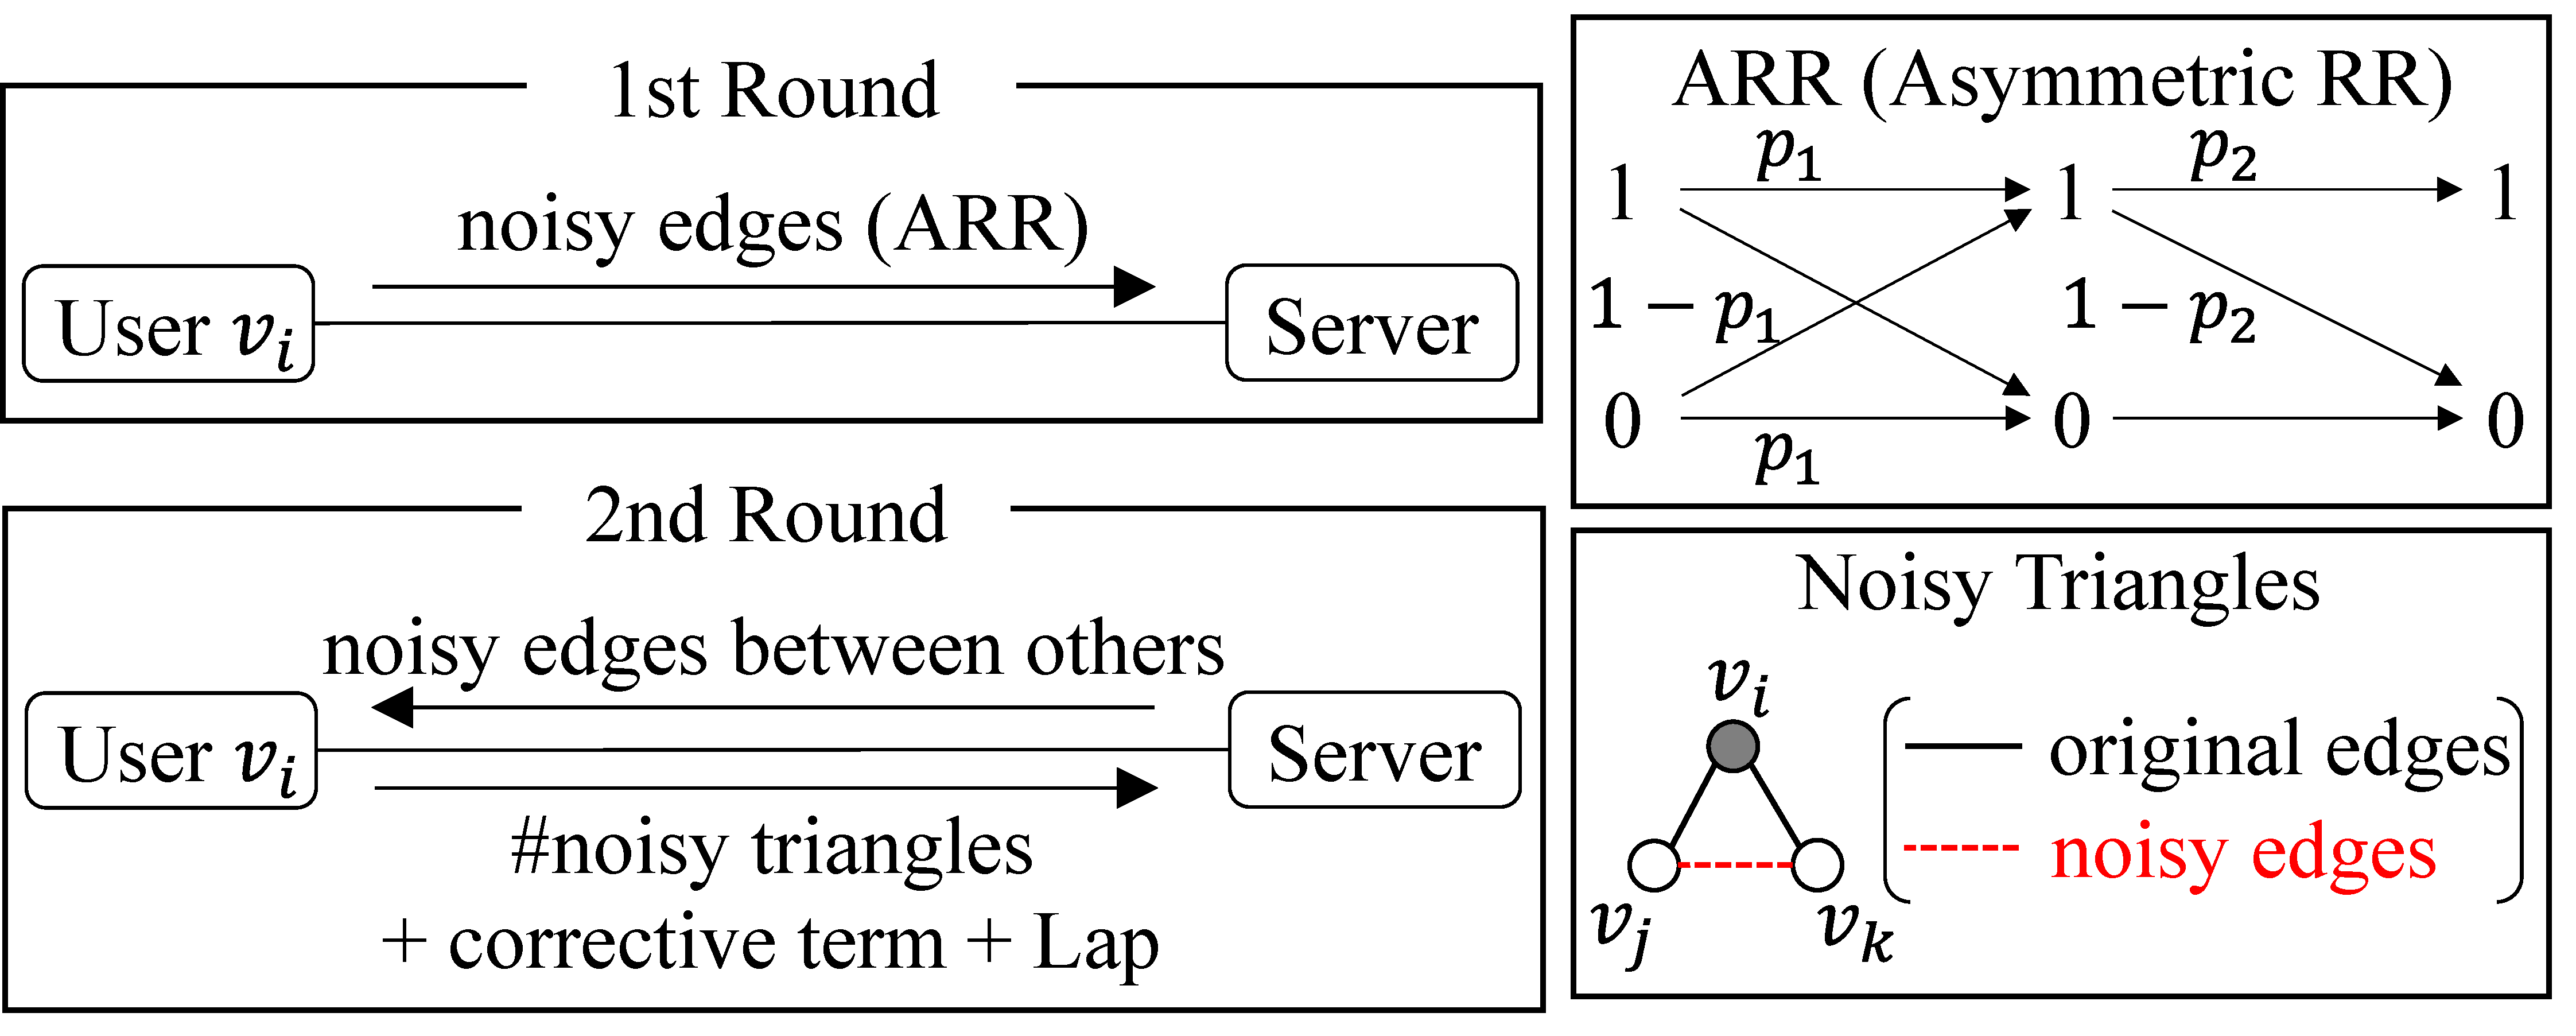
\includegraphics[width=0.99\linewidth]{fig/algorithm_overview.pdf}
  \vspace{-4mm}
  \caption{Overview of our communication-efficient triangle counting algorithms
  ($p_1 =\frac{e^{\epsilon}}{e^{\epsilon}+1}$,
  %$p_1 \in [\frac{1}{2},1]$,
  $p_2 \in [0,1]$).}
  %($\mu \in [0,1]$, $\rho = e^{-\epsilon_1}$).}
  %At the first round, each user obfuscates her edge by ARR ($\mu \in [0,1]$, $\rho \in e^{-\epsilon_1}$) to provide $\epsilon_1$-edge LDP.
  \label{chap2-fig:alg_overview}
\end{figure}

% \smallskip
% \noindent{\textbf{Our Two-Rounds Algorithms.}}~~
\smallskip
\noindent{\textbf{Algorithm Overview.}}~~Figure~\ref{chap2-fig:alg_overview} shows the overview of our proposed algorithms.
% all of which are run in two rounds.
% Below we explain the overview of our algorithms\footnote{For ease of explanation, we explain algorithms that use all elements in $\bmA$ in Section~\ref{chap2-sub:algorithms_overview}.
% In Section~\ref{chap2-sub:three_algorithms}, we propose algorithms that use only the lower triangular part of $\bmA$ to avoid the doubling issue, as described in Section~\ref{chap2-sub:LDP}.}.

At the first round, each user $v_i$ obfuscates
% $i-1$ bits for smaller user IDs in her neighbor list $\bma_i$ (i.e., lower triangular part of $\bmA$)
% each bit of her neighbor list $\bma_i$
% (for users with smaller user IDs)
bits for smaller user IDs in her neighbor list $\bma_i$
% (i.e., lower triangular part of $\bmA$)
by an LDP mechanism which we call the \textit{ARR (Asymmetric Randomized Response)} 
and sends the obfuscated bits to a server. 
% (note that we use only the lower triangular part of $\bmA$ to avoid the doubling issue, as described in Section~\ref{chap2-sub:LDP}).
The ARR is a combination of Warner's RR and edge sampling; i.e.,
we apply Warner's RR that outputs 1 or 0 as it is with probability
% $p_1\in[\frac{1}{2},1]$
$p_1$ ($=\frac{e^{\epsilon}}{e^{\epsilon}+1}$)
and then sample each 1 with probability $p_2\in[0,1]$.
%
% Given 1 (resp.~0) as input, the ARR outputs 1 with probability $\mu$ (resp.~$\mu\rho$), where $\mu \in [0,1]$, $\rho = e^{-\epsilon_1}$, and $\epsilon_1 \in \nnreals$.
% We can view this mechanism as a combination of Warner's RR~\cite{Warner_JASA65} and edge sampling; i.e., we apply Warner's RR that
% outputs 1 or 0 as it is with probability $p_1=\frac{e^{\epsilon_1}}{e^{\epsilon_1}+1}$
% and then sample each 1 with probability $p_2\in[0,1]$, where $\mu=p_1 p_2$.
% In fact, the ARR with $\mu = p_1$ (i.e., $p_2=1$) is equivalent to Warner's RR.
Unlike Warner's RR, the ARR is asymmetric in that the flip probability in the whole process is different
depending on the input value.
As with Warner's RR, the ARR provides edge LDP.
% Since Warner's RR provides
% $\epsilon_1$-
% edge LDP (as described in Section~\ref{chap2-sub:LDP}) and
% the sampling is a post-processing process (and
% DP is immune to post-processing~\cite{DP}, the ARR also provides
% $\epsilon_1$-
% edge LDP.
We can also significantly reduce the number of 1s (hence the communication cost) by setting
% the sampling probability
$p_2$ small.
% $\mu$ much smaller than $p_1$.
% Let $E' \subseteq V \times V$ be a set of noisy edges sent by users.

At the second round, the server calculates a message $M_i$ for user $v_i$ consisting of some or all noisy edges between others. 
We propose three strategies for calculating $M_i$. 
% and
% each user
User $v_i$ downloads $M_i$ from the server.
% a message $M_i$ from the server consisting of some or all
% of $E'$.
% noisy edges between others.
Then, since user $v_i$ knows her edges, $v_i$ can count \textit{noisy triangles} ($v_i$, $v_j$, $v_k$) such that $j<k<i$ and only one edge ($v_j$, $v_k$) is noisy, as shown in Figure~\ref{chap2-fig:alg_overview}. 
% $(v_i,v_j) \in E$, $(v_i,v_k) \in E$,
% $(v_j,v_k) \in E'$, and $j<k<i$;
% i.e., only one edge is noisy
The condition $j<k<i$ is imposed to use only the lower triangular part of $\bmA$, i.e., 
to avoid the doubling issue in Section~\ref{chap2-sub:LDP}. 
% Then $v_i$ adds some post-processing (to enable the server to obtain an unbiased estimate of $f_\triangle(G)$) and the Laplacian noise (to provide $\epsilon_2$-edge LDP for $\epsilon_2 \in \nnreals$) to the noisy triangle count, and sends it to a server.
User $v_i$ adds %some post-processing
a corrective term
%(to enable the server to obtain an unbiased estimate of $f_\triangle(G)$) 
and the Laplacian noise
% (to provide edge LDP)
to the noisy triangle count 
and sends it to a server.
The corrective term is added to enable the server to obtain an unbiased estimate of $f_\triangle(G)$. 
The Laplacian noise provides
% $\epsilon_2$-
edge LDP.
% , where $\epsilon_2 \in \nnreals$.
% From this,
Finally,
the server calculates an unbiased estimate of $f_\triangle(G)$
from the noisy data sent by users.
By composition (Proposition~\ref{chap2-prop:seq_comp_edge_LDP}),
% the compositionality of DP~\cite{DP},
our algorithms provide
% ($\epsilon_1 + \epsilon_2$)-
edge LDP in total.

\smallskip
\noindent{\textbf{Remark.}}~~Note that it is also possible for the server to calculate an unbiased estimate of $f_\triangle(G)$ at the first round.
However, this results in a
prohibitively
% very
large estimation error
% for a large graph
% for two reasons.
because
% First,
all edges sent by users are noisy; i.e., three edges are noisy in any triangle.
% all three edges are noisy in any triangle at the first round (whereas only one edge is noisy in our algorithms),
% Second, the noisy graph is dense, and consequently the time complexity of counting noisy triangles is $O(n^3)$. Thus, some approximation (such as edge sampling) is necessary to efficiently compute the estimate of $f_\triangle(G)$.
In contrast, only one edge is noisy in each noisy triangle at the second round because each user $v_i$ knows two original edges
% $(v_i,v_j) \in E$ and $(v_i,v_k) \in E$
connected to $v_i$.
Consequently, we can obtain an unbiased estimate with a much smaller variance.
See Appendix~\ref{chap2-sec:one-round} for a detailed comparison.
% In Appendix~\ref{chap2-sec:one-round}, we show that
% our two-rounds algorithms significantly outperform the existing one-round triangle algorithms.
% ~\cite{Imola_USENIX21,Ye_TKDE21}.
% (with sampling).
% the estimation error is significantly reduced by introducing an additional round.

% \subsection{Three Algorithms}
\subsection{Algorithms}
\label{chap2-sub:three_algorithms}

\smallskip
\noindent{\textbf{ARR.}}~~First, we formally define the ARR.
% We begin with a formal definition of the ARR.
% Below we describe our algorithms in detail.
The ARR has two parameters: $\epsilon \in \nnreals$ and $\mu \in [0,\frac{e^{\epsilon}}{e^{\epsilon} + 1}]$.
The parameter $\epsilon$ is the privacy budget, and $\mu$ controls the communication cost.

Let
% $\calR_{ARR}$
$ARR_{\epsilon,\mu}$ be the ARR with parameters $\epsilon$ and $\mu$. It takes $0/1$ as input and outputs $0/1$ with the following probability:
\begin{align}
    \Pr[ARR_{\epsilon,\mu}(1) = b] &= \begin{cases}\mu & (b=1) \\ 1-\mu & (b=0)\end{cases} \label{chap2-eq:ARR_1}\\
    \Pr[ARR_{\epsilon,\mu}(0) = b] &= \begin{cases}\mu\rho & (b=1) \\ 1-\mu \rho & (b=0), \end{cases} \label{chap2-eq:ARR_0}
\end{align}
where $\rho = e^{-\epsilon}$.
By Figure~\ref{chap2-fig:alg_overview},
we can view this randomizer as a combination of Warner's RR~\cite{Warner_JASA65}
% with $p_1=\frac{e^{\epsilon}}{e^{\epsilon}+1}$
and edge sampling, where $\mu=p_1 p_2$.
In fact, the ARR with $\mu = p_1 =\frac{e^{\epsilon}}{e^{\epsilon}+1}$ (i.e., $p_2=1$) is equivalent to Warner's RR.

Each user $v_i$ applies the ARR to bits for smaller user IDs in her neighbor list $\bma_i$; i.e., $\calR_i(\bma_i) = (ARR_{\epsilon,\mu}(a_{i,1}), \ldots, \allowbreak ARR_{\epsilon,\mu}(a_{i,i-1}))$.
% Note that we use only the lower triangular part of $\bmA$ to avoid the doubling issue described in Section~\ref{chap2-sub:LDP}.
Then $v_i$ sends $\calR_i(\bma_i)$ to the server.
% Applying Warner's RR to each bit of $\bma_i$ provides $\epsilon$-edge LDP (as described in Section~\ref{chap2-sub:LDP}).
Since applying Warner's RR to $\bma_i$ provides $\epsilon$-edge LDP (as described in Section~\ref{chap2-sub:LDP}) and the sampling is a post-processing process, applying the ARR to $\bma_i$ also provides $\epsilon$-edge LDP by the immunity to post-processing~\cite{DP}.

Let $E' \subseteq V \times V$ be a set of noisy edges sent by users.

\smallskip
\noindent{\textbf{Which Noisy Edges to Download?}}~~Now, the main question
tackled in this paper is: \textit{Which noisy edges should each user $v_i$
download at the second round?}
Note that
% user $v_i$ cannot leak her original edges to the server.
% For example,
user $v_i$
% cannot
is not allowed to
download only a set of noisy edges that form noisy triangles
(i.e., $\{(v_j,v_k) \in E' | (v_i,v_j) \in E, (v_i,v_k) \in E$\}),
% a set of noisy edges $\{(v_j,v_k) \in E' | (v_i,v_j) \in E, (v_i,v_k) \in E$\} (i.e., only noisy edges that form noisy triangles),
because it tells the server
% the fact that $v_j$ and $v_k$ are friends with $v_i$.
who are friends with $v_i$.
In other words, user $v_i$ cannot leak her original edges to the server when she
downloads noisy edges; the server must choose which part of $E'$ to include in
the message $M_i$ it sends her.

Thus, a natural solution would be to download \textit{all noisy edges between others}
% (except for the ones connected to $v_i$).
(with smaller user IDs); i.e.,
% \begin{align}
% M_i =\{(v_j, v_k) \in E' | j<k<i\}. \label{chap2-eq:M_i_I}
% \end{align}
$M_i =\{(v_j, v_k) \in E' | j<k<i\}$.
% as shown in Figure~\ref{chap2-fig:noisy_edge_DL}.
We denote our algorithm with this full download strategy by \AlgOne{}.
The (inefficient) two-rounds algorithm in~\cite{Imola_USENIX21} is a special case of \AlgOne{}
without sampling ($\mu = p_1$).
% when $\mu = p_1$ (i.e., when we
% use Warner's RR and
% do not sample edges).
In other words, \AlgOne{} is a generalization of the two-rounds algorithm in~\cite{Imola_USENIX21} using the ARR.
% $(v_j,v_k) \in E'$ such that $(v_i,v_j) \in E$, $(v_i,v_k) \in E$
% The expected download size in \AlgOne{} is $O(\mu n^2)$.

% Since users have already sent noisy edges at the first round, user $v_i$ can use noisy edges connected to $v_i$ when downloading noisy edges.
% For example,

In this paper,
we show that we can do much better
% we achieve much higher utility
than \AlgOne{}.
Specifically, we prove in Section~\ref{chap2-sub:algorithms_theoretical_analysis} that \AlgOne{} results in a high estimation error when the number of 4-cycles (cycles of length 4) in $G$ is large.
Intuitively, this can be explained as follows.
Suppose that $v_i$, $v_j$, $v_{i'}$, and $v_k$
($j<k<i$, $j<k<i'$)
form a 4-cycle. 
% $v_i-v_j-v_{i'}-v_k-v_i$.
% (denoted by $v_i$-$v_j$-$v_{i'}$-$v_k$).
% , as shown in the left panel of Figure~\ref{chap2-fig:four-cycle}.
There is no triangle in this graph.
However, if there is a noisy edge between $v_j$ and $v_k$, then two (incorrect) noisy triangles appear: ($v_i$, $v_j$, $v_k$) counted by $v_i$ and ($v_{i'}$, $v_j$, $v_k$) counted by $v_{i'}$.
More generally, let $E_{ijk}$ (resp.~$E_{i'jk}$) $\in \{0,1\}$ be a random variable that takes $1$ if ($v_i$, $v_j$, $v_k$) (resp.~($v_{i'}$, $v_j$, $v_k$)) forms a noisy triangle and $0$ otherwise.
Then, the covariance $\cov(E_{ijk},E_{i'jk})$ between $E_{ijk}$ and $E_{i'jk}$ is large because the presence/absence of a single noisy edge ($v_j$, $v_k$) affects the two noisy triangles.

To address this issue, we introduce a
% \textit{trick}
trick 
% trick, which we call the ``$4$-cycle trick'',
that makes the two noisy triangles \textit{less correlated with each other}.
We call this the \textit{4-cycle trick}.
% Since users have already sent noisy edges at the first round,
% user $v_i$ can use noisy edges connected to $v_i$ when downloading noisy edges.
Specifically,
% we propose two algorithms: \AlgTwo{} and \AlgThree{}.
we propose two algorithms in which
% user $v_i$ uses noisy edges connected to $v_i$ when downloading noisy edges.
the server uses noisy edges connected to $v_i$ when it calculates a message $M_i$ for $v_i$.
In the first algorithm,
% user $v_i$ downloads
the server selects
noisy edges $(v_j, v_k)$ such that
one noisy edge is connected from $v_k$ to $v_i$;
% there is a noisy edge between $v_i$ and $v_k$;
i.e.,
$M_i = \{(v_j, v_k) \in E' | (v_i, v_k) \in E', j<k<i\}$.
% \begin{align}
% M_i = \{(v_j, v_k) \in E' | (v_i, v_k) \in E', j<k<i\}. \label{chap2-eq:M_i_II}
% \end{align}
We call this algorithm \AlgTwo{}, as one noisy edge is connected to $v_i$.
In the second algorithm,
% user $v_i$ downloads
the server selects
noisy edges $(v_j, v_k)$ such that
two noisy edges are connected from these nodes to $v_i$; i.e.,
$M_i = \{(v_j, v_k) \in E' | (v_i, v_j) \in E', (v_i, v_k) \in E', j<k<i\}$.
% \begin{align}
% \hspace{-2mm} M_i \hspace{-0.5mm} = \hspace{-0.5mm}  \{(v_j, v_k) \in E' | (v_i, v_j) \in E', (v_i, v_k) \in E', j<k<i\}. \label{chap2-eq:M_i_III}
% \end{align}
We call this algorithm \AlgThree{}, as two noisy edges are connected to $v_i$.
Note that user $v_i$ does not leak her original edges to the server at the time of download in these algorithms, because
% $v_i$ uses only noisy edges the server has.
the server uses only noisy edges $E'$ sent by users to calculate $M_i$.

Figure~\ref{chap2-fig:noisy_edge_DL} shows our three algorithms.
% Let $\mu_F, \mu_O, \mu_T \in \nnreals$ be values of $\mu$ in the ARR used for \AlgOne{}, \AlgTwo{}, and \AlgThree{}, respectively.
% Then the
The download cost $\CostDL{}$ in (\ref{chap2-eq:cost_DL}) is
$O(\mu n^2 \log n)$, $O(\mu^2 n^2 \log n)$, and $O(\mu^3 n^2 \log n)$,
% $O(\mu_F n^2 \log n)$, $O(\mu_O^2 n^2 \log n)$, and $O(\mu_T^3 n^2 \log n)$,
respectively, when we regard $\epsilon$ as a constant.
In our experiments, we set
the parameter $\mu$ in the ARR so that
% $\mu$ in \AlgOne{}, $\mu^2$ in \AlgTwo{}, and $\mu^3$ in \AlgThree{} are equal
$\mu$ in \AlgOne{} is equal to $\mu^2$ in \AlgTwo{} and also equal to $\mu^3$ in \AlgThree{};
e.g., $\mu=10^{-6}$, $10^{-3}$, and $10^{-2}$ in \AlgOne{}, \AlgTwo{}, and \AlgThree{}, respectively.
% $\mu_F$, $\mu_O$, and $\mu_T$ to $\mu_F = \mu_O^2 = \mu_T^3$ (e.g., $\mu_F=10^{-6}$, $\mu_O=10^{-3}$, $\mu_T=10^{-2}$)
% so that
% the expected download size
Then
the download cost
is the same between the three algorithms.

\begin{figure}[t]
  \centering
  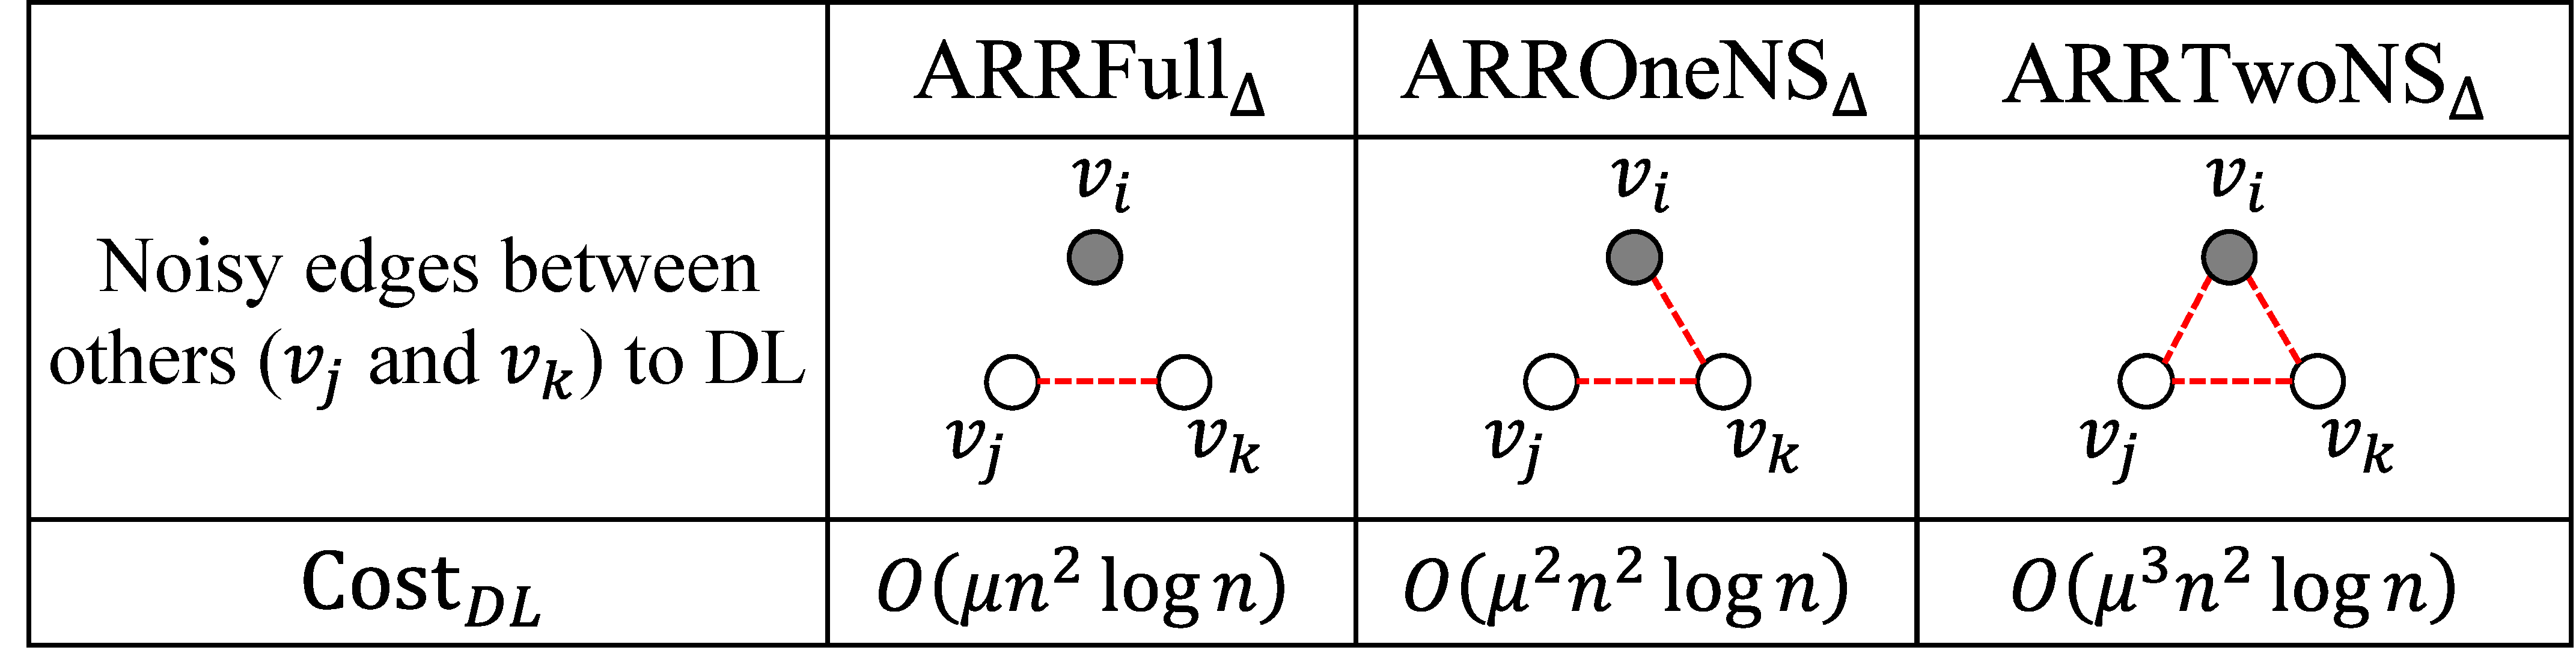
\includegraphics[width=0.99\linewidth]{fig/three_algorithms.pdf}
  \vspace{-4mm}
  \caption{Noisy edges to download
  % and expected download size
  in our three algorithms.}
  %$\mu_F$, $\mu_O$, and $\mu_T$ are values of $\mu$ in the ARR used for \AlgOne{}, \AlgTwo{}, and \AlgThree{}, respectively.}
  \label{chap2-fig:noisy_edge_DL}
% \end{figure}
\vspace{4mm}
% \begin{figure}[t]
  \centering
  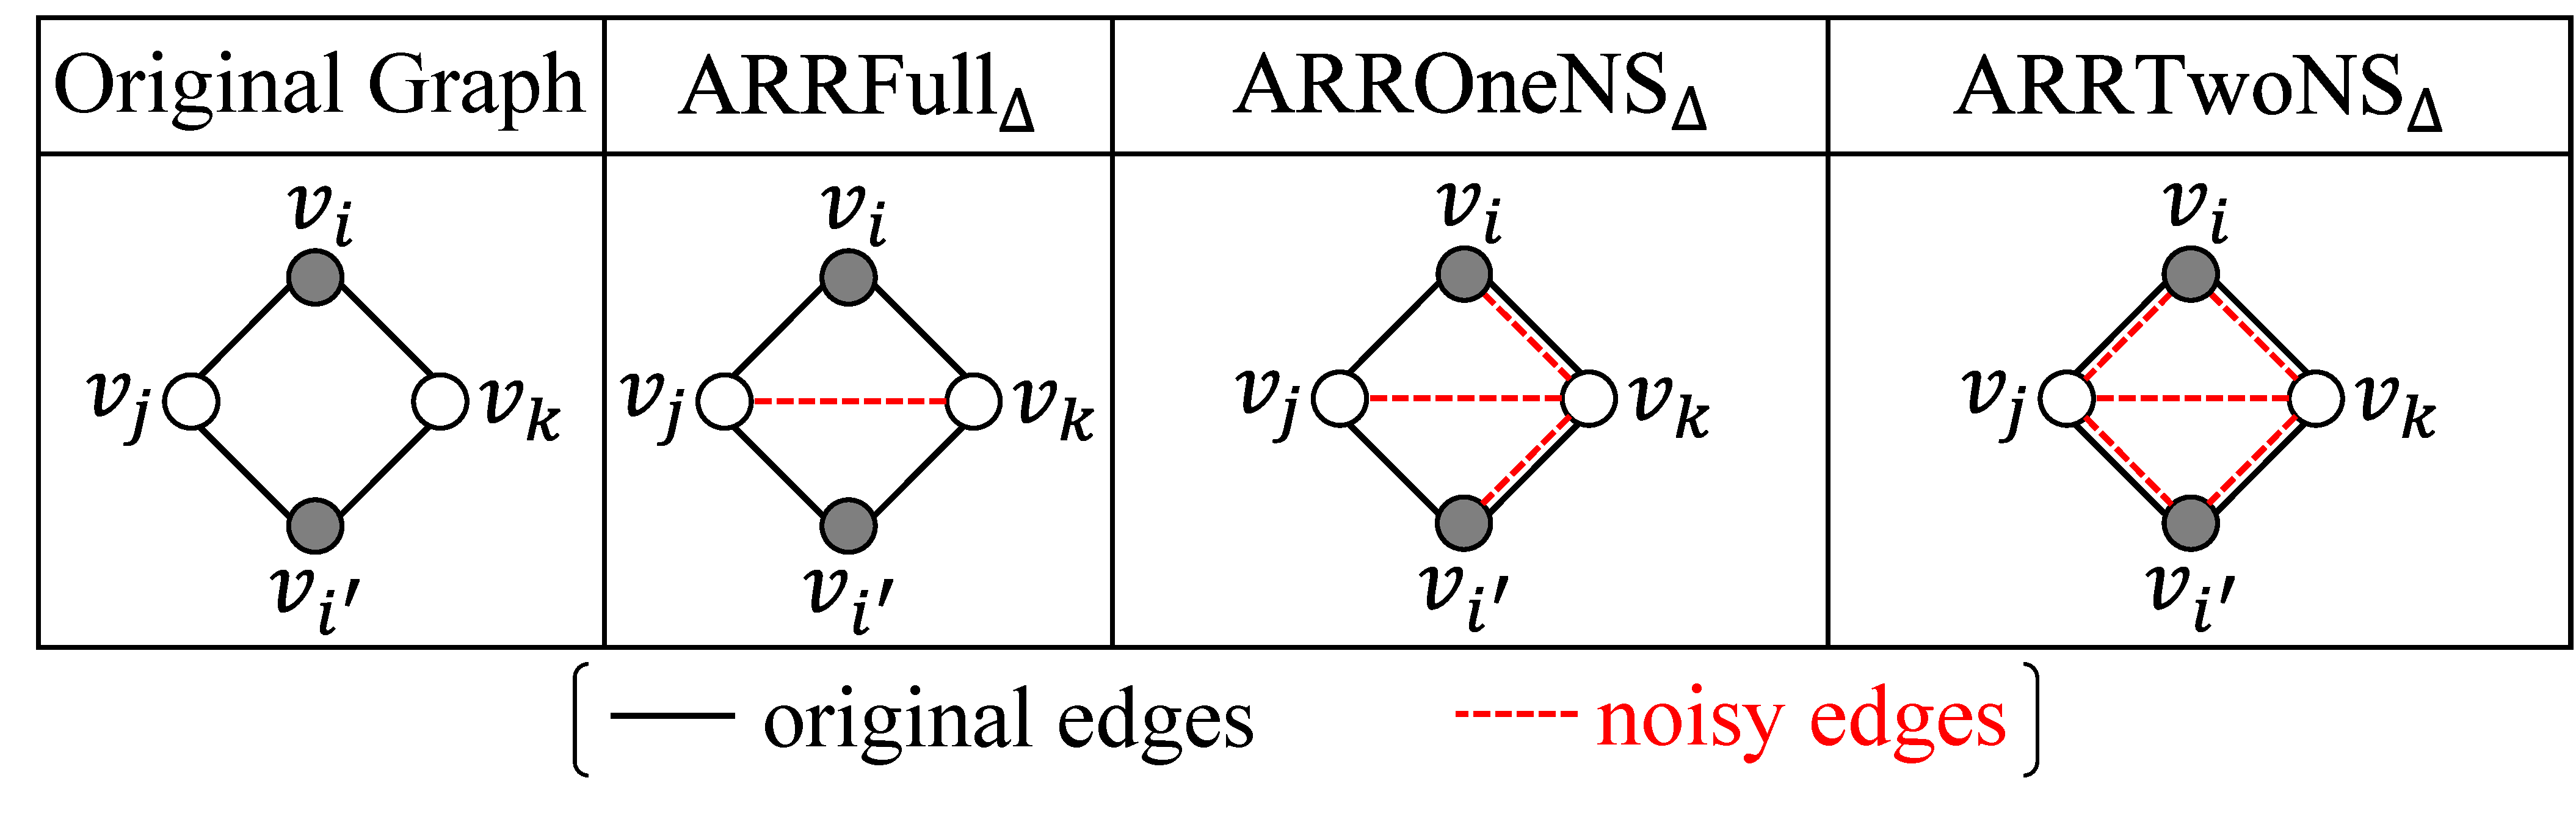
\includegraphics[width=0.95\linewidth]{fig/four_cycle.pdf}
  \vspace{-4mm}
  \caption{4-cycle trick.
  % 4-cycle issue.
  \AlgOne{} counts two (incorrect) noisy triangles when one noisy edge appears.
  \AlgTwo{} and \AlgThree{} avoid this by increasing independent noise.}
  \label{chap2-fig:four-cycle}
\end{figure}

% Figure\ref{chap2-fig:four-cycle} shows why and how \AlgTwo{} and \AlgThree{} address the 4-cycle issue.
Figure~\ref{chap2-fig:four-cycle} shows our $4$-cycle trick.
\AlgOne{} counts two (incorrect) noisy triangles when a noisy edge ($v_j$, $v_k$) appears.
% there is a noisy edge ($v_j$, $v_k$).
In contrast,
% the two noisy triangles are counted
\AlgTwo{} (resp.~\AlgThree{}) counts both the two noisy triangles
% this bad event happens
only when three (resp.~five) independent noisy edges appear,
% in \AlgTwo{} (resp.~\AlgThree{}),
as shown in Figure~\ref{chap2-fig:four-cycle}.
% Since these noisy edges are independent,
Thus, this bad event happens with a much smaller probability.
For example,
% when $\mu_F=10^{-6}$, $\mu_O=10^{-3}$, and $\mu_T=10^{-2}$,
% \AlgOne{}, \AlgTwo{}, and \AlgThree{} count both the two noisy triangles with probability $10^{-6}$, $10^{-9}$, and $10^{-10}$, respectively.
\AlgOne{} ($\mu=10^{-6}$),
\AlgTwo{} ($\mu=10^{-3}$), and
\AlgThree{} ($\mu=10^{-2}$)
count both the two noisy triangles with probability $10^{-6}$, $10^{-9}$, and $10^{-10}$, respectively.
The covariance $\cov(E_{ijk},E_{i'jk})$ of \AlgTwo{} and \AlgThree{} is also much smaller than that of \AlgOne{}.
% \AlgTwo{} and \AlgThree{} also achieve much smaller covariance $\cov(E_{ijk},E_{i'jk})$ than \AlgOne{}.


In our experiments, we show that \AlgTwo{} and \AlgThree{} significantly outperforms \AlgOne{}
% in two real graph datasets with a large number of 4-cycles.
for a large-scale graph or dense graph, in both of which
% when
the number of 4-cycles in $G$ 
% can be very 
is 
large.
% \ji{Are there other scenarios where the performance is better?}
% \commentT{I think the number of 4-cycles can be large when a graph is (i) large or (ii) dense (in particular, (i) is important). I clarified this.}

\smallskip
\noindent{\textbf{\AlgTwo{} vs. \AlgThree{}.}}~~One
% The number of independent noisy edges in a 4-cycle is three and five in \AlgTwo{} and \AlgThree{}, respectively, as shown in Figure\ref{chap2-fig:four-cycle}.
% Thus
might expect that \AlgThree{} outperforms \AlgTwo{} because \AlgThree{} addresses the 4-cycle issue more aggressively; i.e.,
% \AlgThree{} has the largest number of independent noisy edges in a 4-cycle,
the number of independent noisy edges in a 4-cycle is larger in \AlgThree{},
as shown in Figure \ref{chap2-fig:four-cycle}.
However,
% \AlgThree{} suffers from a large global sensitivity of the Laplacian noise at the second round.
\AlgTwo{} can reduce the global sensitivity of the Laplacian noise
at the second round
more effectively than \AlgThree{}, as explained in Section~\ref{chap2-sec:double_clip}.
% in detail.
Consequently, \AlgTwo{}, which is the most tricky algorithm, achieves the smallest estimation error in our experiments.
See Sections~\ref{chap2-sec:double_clip} and \ref{chap2-sec:experiments} for details of the global sensitivity and experiments, respectively.

\smallskip
\noindent{\textbf{Three Algorithms.}}~~Below we explain the details of our three algorithms.
For ease of explanation, we assume that the maximum degree $d_{max}$ is public in Section~\ref{chap2-sub:three_algorithms}\footnote{For example, $d_{max}$ is public in Facebook: $d_{max} = 5000$~\cite{Facebook_Limit}.
If the server does not have prior knowledge about $d_{max}$, she can privately estimate $d_{max}$ and use graph projection to guarantee that each user's degree never exceeds the private estimate of $d_{max}$~\cite{Imola_USENIX21}.
In any case, the assumption in Section~\ref{chap2-sub:three_algorithms} does not undermine our algorithms, because our entire algorithms with double clipping in Section~\ref{chap2-sec:double_clip} does \textit{not} assume that $d_{max}$ is public.}.
Note, however, that
% we propose a technique to significantly reduce the global sensitivity
our double clipping (which is proposed to significantly reduce the global sensitivity) in Section~\ref{chap2-sec:double_clip} does \textit{not} assume that $d_{max}$ is public.
Consequently, our entire algorithms 
% (i.e., \AlgOne, \AlgTwo, \AlgThree with double clipping)
% three triangle counting algorithms (\AlgOne, \AlgTwo, \AlgThree) with our double clipping
do \textit{not} require the assumption that $d_{max}$ is public.

\setlength{\algomargin}{5mm}
\begin{algorithm}[t]
  \SetAlgoLined
  \KwData{Graph $G \in \calG$ represented as neighbor lists $\bma_1, \ldots, \bma_n
    \in \{0,1\}^n$, privacy budgets
  $\epsilon_1,\epsilon_2 \in \nnreals$, $d_{max} \in \nnints$,
  $\mu \in [0,\frac{e^{\epsilon_1}}{e^{\epsilon_1} + 1}]$.
  %$\mu^*$.
  }
  \KwResult{Private estimate $\hf_\triangle(G)$ of $f_\triangle(G)$.}
%   $p_1 \leftarrow \frac{1}{e^{\epsilon_1}}$\;
  [s] $\rho \leftarrow e^{-\epsilon_1}$\;
  [$v_i$, s] $\mu^* \leftarrow \mu$, $\mu^2$, and $\mu^3$ in F, O, and T, respectively\;
  \tcc{First round.}
  \For{$i=1$ \KwTo $n$}{
    [$v_i$] $\bmr_i \leftarrow (ARR_{\epsilon_1,\mu}(a_{i,1}), \ldots,
    ARR_{\epsilon_1,\mu}(a_{i,i-1}))$\;
    [$v_i$] Upload $\bmr_i = (r_{i,1}, \ldots, r_{i,i-1})$ to the server\;
  }
%   $E' = \{(v_i, v_j) : i > j, r_{i,j} = 1\} \cup \{(v_j, v_i) : i > j, r_{i,j} =
%   1\}$\;
  [s] $E' = \{(v_j, v_k) :r_{k,j} = 1, j < k\}$\;
  \tcc{Second round.}
  \For{$i=1$ \KwTo $n$}{
    [s] Compute
    $M_i$ by (\ref{chap2-eq:M_i_I}), (\ref{chap2-eq:M_i_II}), and (\ref{chap2-eq:M_i_III}) in F, O, and T, respectively\;
    %$M_i = \{(v_j,v_k) \in E': j < k < i\}$\;
    %$M_i = \{(v_j,v_k) \in E': (v_i,v_k) \in E', j < k < i\}$\;
    %$M_i = \{(v_j,v_k) \in E': (v_i,v_k), (v_j,v_k) \in E', j < k < i\}$\;
    [$v_i$] Download $M_i$ from the server\;
    [$v_i$] $t_i \leftarrow |\{(v_i,v_j,v_k) :
    a_{i,j} = a_{i,k} = 1, (v_j,v_k) \in M_i, j<k<i \}|$\;
    [$v_i$] $s_i \leftarrow |\{(v_i,v_j,v_k) :
    a_{i,j} = a_{i,k} = 1, j<k<i\}|$\;
    [$v_i$] $w_i \leftarrow t_i - \mu^* \rho s_i$\;
    [$v_i$] $\hw_i \leftarrow w_i + \Lap(\frac{d_{max}}{\epsilon_2})$\;
    [$v_i$] Upload $\hw_i$ to the server\;
  }
  [s] $\hf_\triangle(G) \leftarrow \frac{1}{\mu^*(1-\rho)}\sum_{i=1}^n \hw_i$\;
  \KwRet{$\hf_\triangle(G)$}
  \caption{Our three algorithms.
  ``F'', ``O'', ``T'' are shorthands for
  %$\mu^*=\mu_F$, $\mu_O^2$, and $\mu_T^3$ in
  \AlgOne{}, \AlgTwo{}, and \AlgThree{}, respectively.
  [$v_i$] and [s] represent that the process is run by $v_i$ and the server, respectively.
  }\label{chap2-alg:unify}
\end{algorithm}

% As explained above,
Recall that the server calculates a message $M_i$ for $v_i$ as:
\begin{align}
\hspace{-1mm} M_i \hspace{-0.5mm} &= \hspace{-0.5mm} \{(v_j, v_k) \in E' | j<k<i\} \label{chap2-eq:M_i_I}\\
\hspace{-1mm} M_i \hspace{-0.5mm} &= \hspace{-0.5mm} \{(v_j, v_k) \in E' | (v_i, v_k) \in E', j<k<i\} \label{chap2-eq:M_i_II}\\
\hspace{-1mm} M_i \hspace{-0.5mm} &= \hspace{-0.5mm}  \{(v_j, v_k) \in E' | (v_i, v_j) \in E', (v_i, v_k) \in E', j<k<i\} \label{chap2-eq:M_i_III}
\end{align}
in \AlgOne{}, \AlgTwo{}, \AlgThree{}, respectively.

%Using these equations,
% our three algorithms can be unified in Algorithm~\ref{chap2-alg:unify}.
Algorithm~\ref{chap2-alg:unify} shows our three algorithms.
These algorithms are processed differently in lines 2 and 9; ``F'', ``O'', ``T'' are shorthands for \AlgOne{}, \AlgTwo{}, and \AlgThree{}, respectively.
% It uses two rounds of private computation, and
% in both rounds each user $v_i$ applies a local randomizer to her neighbor list $\bma_i$.
The privacy budgets for the first and second
rounds are $\epsilon_1, \epsilon_2 \in \nnreals$, respectively.

The first round appears in lines 3-7 of Algorithm~\ref{chap2-alg:unify}.
In this round, each user applies
$ARR_{\epsilon_1, \mu}$
% the ARR
defined by (\ref{chap2-eq:ARR_1}) and (\ref{chap2-eq:ARR_0}) to bits $a_{i,1}, \ldots, a_{i,i-1}$ for smaller user IDs in her neighbor list $\bma_i$, i.e., lower triangular part of $\bmA$.
% explained in the beginning of
% Section~\ref{chap2-sub:three_algorithms}.
Let $\bmr_i = (r_{i,1}, \ldots, r_{i,i-1}) \in \{0,1\}^{i-1}$ be the obfuscated bits of $v_i$.
User $v_i$ uploads $\bmr_i$ to the server.
Then the server combines the noisy edges together, forming $E' = \{(v_j, v_k) : r_{k,j} = 1, j < k\}$.

The second round appears in lines 8-17 of Algorithm~\ref{chap2-alg:unify}.
In this round, the server computes a message $M_i$
by (\ref{chap2-eq:M_i_I}), (\ref{chap2-eq:M_i_II}), or (\ref{chap2-eq:M_i_III}),
% depending on the algorithm,
and user $v_i$ downloads it.
% As explained above, \AlgOne{}, \AlgTwo{}, and \AlgThree{} computes $M_i$ by (\ref{chap2-eq:M_i_I}), (\ref{chap2-eq:M_i_II}), and  (\ref{chap2-eq:M_i_III}), respectively.
Then user $v_i$ calculates the number $t_i \in \nnints$ of noisy triangles ($v_i$, $v_j$, $v_k$) such that
% $j<k<i$ and
only one edge ($v_j$, $v_k$) is noisy, as shown in Figure~\ref{chap2-fig:alg_overview}.
% involving two edges in user $v_i$'s neighbor list and one noisy edge in $E'$ (as shown in Figure~\ref{chap2-fig:alg_overview}).
% We also emphasize that the condition $j<k<i$ is imposed to use only the lower triangular part of $\bmA$.
% (and avoid the doubling issue).
User $v_i$ also calculate a corrective term $s_i \in \nnints$.
The corrective term $s_i$ is the number of
possible triangles involving $v_i$ 
% that can be formed from edges in $v_i$'s neighbor list,
and is computed to obtain an unbiased estimate of $f_\triangle(G)$.
% unbias the triangle count.
User $v_i$ calculates $w_i = t_i - \mu^* \rho s_i$, where $\rho = e^{-\epsilon_1}$ and
% $\mu^* = \mu_F$, $\mu_O^2$, and $\mu_T^3$
$\mu^* = \mu$, $\mu^2$, and $\mu^3$
in ``F'', ``O'', and ``T'', respectively.
% \AlgOne{}, \AlgTwo{}, and \AlgThree{}, respectively.
Then $v_i$ adds the Laplacian noise $\Lap(\frac{d_{max}}{\epsilon_2})$ to $w_i$ to provide $\epsilon_2$-edge LDP and sends the noisy value $\hw_i$ ($= w_i + \Lap(\frac{d_{max}}{\epsilon_2})$) to the server. 
Note that adding one edge increases both $t_i$ and $s_i$ 
% results in the increase of the triangle count 
by at most $d_{max}$. 
Thus, the global sensitivity of $w_i$ is at most $d_{max}$. 
Finally, the server calculates an estimate of $f_\triangle(G)$ as: $\hf_\triangle(G) = \frac{1}{\mu^*(1-\rho)}\sum_{i=1}^n \hw_i$.
As we prove later, $\hf_\triangle(G)$ is an unbiased estimate of $f_\triangle(G)$.

% \smallskip
% \noindent{\textbf{\AlgOne.}}

% Our first algorithm, \AlgOne, appears in Algorithm~\ref{chap2-alg:one}. It uses two
% rounds of private computation, and in both rounds each user applies a local
% randomizer to his data.
% The privacy budgets for the two
% rounds are $\epsilon_1, \epsilon_2$.

% The first round appears in Lines 3-4 of Algorithm~\ref{chap2-alg:one}. This round
% collects the noisy edges from the users.
% The noisy edges are produced
% using the asymmetric randomized response mechanism, which we denote
% $ARR_{\epsilon, \mu}$. Recall that a bit $a_{i,j}$ of $\bma_i$ takes value $1$
% if and only if user $v_i$ includes user $v_j$ in his neighbor list. ARR is
% defined by $\Pr[ARR_{\epsilon, \mu}(1) = 1] = \mu$ and $\Pr[ARR_{\epsilon,
% \mu}(0) = 1] = \mu p_1$ where $p_1 = e^{-\epsilon_1}$. User $v_i$ uploads
% $\bmr_i$, the vector of ARR mechanisms applied to $a_{i,j}$ for $j < i$. This
% means that user $v_i$ ignores users with a bigger index than $i$. By doing so,
% for every possible undirected edge $(v_i, v_j)$, exactly one of $v_i, v_j$ will
% upload the
% edge using ARR. This prevents releasing the edge twice, and allows us to prove
% that our mechanism satisfies relationship DP without the doubling factor in
% $\epsilon$ (see Proposition~\ref{chap2-prop:edge_LDP_entire_edge_LDP}).
% Given the collection of ARR queries to the users, the server concludes the first
% round by combining the noisy edges together and unordering them, forming $E'$.

% The second round appears in Lines 8-13 of Algorithm~\ref{chap2-alg:one}.
% In this round, each user $v_i$ computes an unbiased estimator $w_i$ for
% the number of triangles involving $v_i$ for which the maximum index of the
% triangle is $i$. It is easy to see that the sum of the $w_i$ estimates the total
% number of triangles. The user does this by
% downloading the message $M = E'$ from the server
% and computing a noisy triangle count $t_i$ and a corrective term $s_i$. The count
% $t_i$ is the number of triangles involving two edges in user $v_i$'s neighbor
% list and one noisy edge in $E'$. The corrective term $s_i$ is the number of
% possible triangles that can be formed from edges in user $v_i$'s neighbor list,
% and is computed to unbias the triangle count. We emphasize that user $v_i$
% only considers the part of his neighbor list involving users of a lower index
% than $i$ for all calculations, including this. The unbiased estimator is
% given by $w_i = t_i - \mu_F p_1 s_i$---because it depends on the private data
% $\bma_i$, the user adds Laplacian noise of width $\frac{d_{max}}{\epsilon_2}$ to
% $w_i$ that the computation may satisfy $\epsilon_2$ edge LDP. He then uploads
% the noisy value $\hw_i$, and the server computes the final triangle estimate.

% \begin{algorithm}
%   \SetAlgoLined
%   \KwData{Graph $G$ represented as neighbor lists $\bma_1, \ldots, \bma_n
%     \in \{0,1\}^n$, two privacy budgets
%   $\epsilon_1,\epsilon_2 > 0$, $d_{max} \in \nnints$, sampling parameter
%   $\mu_F$.}
%   \KwResult{Private estimate of $f_\triangle(G)$.}
%   $p_1 \leftarrow \frac{1}{e^{\epsilon_1}}$\;
%   \tcc{First round.}
%   \For{$i=1$ \KwTo $n$}{
%     $\bmr_i \leftarrow (ARR_{\epsilon_1,\mu_F}(a_{i,1}), \ldots,
%     ARR_{\epsilon_1,\mu_F}(a_{i,i-1}))$\;
%     Upload $\bmr_i$ to server\;
%   }
%   $E' = \{(v_j, v_i) : i > j, r_{i,j} = 1\}$\;
%   \tcc{Second round.}
%   \For{$i=1$ \KwTo $n$}{
%     Server lets $M_i = E'$.
%     Download $M_i$ from server\;
%     $t_i \leftarrow |\{(v_i,v_j,v_k) :
%     j<k<i, a_{i,j} = a_{i,k} = 1, (k,j) \in M \}|$\;
%     $s_i \leftarrow |\{(v_i,v_j,v_k) :
%     j<k<i, a_{i,j} = a_{i,k} = 1\}|$\;
%     $w_i \leftarrow t_i - \mu_F p_1 s_i$\;
%     $\hw_i \leftarrow w_i + \Lap(\frac{d_{max}}{\epsilon_2})$\;
%     Upload $\hw_i$ to server\;
%   }
%   \KwRet{$\frac{1}{\mu_F(1-p_1)}\sum_{i=1}^n \hw_i$}
%   \caption{\AlgOne}\label{chap2-alg:one}
% \end{algorithm}

% \smallskip
% \noindent{\textbf{\AlgTwo.}}

% Our second Algorithm, \AlgTwo, appears in Algorithm~\ref{chap2-alg:two}. Like
% \AlgOne, it uses two rounds with budgets $\epsilon_1$ and $\epsilon_2$.
% The first round is identical to \AlgOne, and for brevity, Algorithm~\ref{chap2-alg:two} does not
% include a description of the first round.
% Recall that the goal of the second round is for each user $v_i$ to compute an estimate of the
% number of triangles in which $i$ is the maximum index, which is the variable
% $\hw_i$.
% The difference between \AlgOne and
% \AlgTwo is that in the second round of \AlgTwo (Lines 2-8), a user only downloads a
% subset of edges in
% $E'$: $v_i$ downloads those edges $(v_j, v_k) \in E'$ such that $j < k < i$ and
% $v_i \text{\----} v_k \text{\----} v_j$ are connected in $E'$. The server is
% able to compute these edges since they only depend on the first round release,
% and we denote it with $M_i$. User $v_i$ then computes his estimate $w_i = t_i -
% \mu_O^2 p_1 s_i$, where $t_i$ is and $s_i$ are the same quantities as in
% \AlgOne. The final estimator $w_i = t_i - \mu_O^2
% p_1 s_i$ is an unbiased estimate of the number of triangles for which $i$ is the
% maximum index. User $v_i$ uploads $\hw_i$, given by $w_i$ plus Laplace noise, in
% order to share $w_i$ privately.

% Downloading only some of $E'$, depending on the noisy first round, actually
% produces a noisier estimator $\hw_i$ than \AlgOne. However, the communication
% cost of \AlgTwo is less, precisely because a subset of $E'$ is downloaded. It
% is straightforward to prove that in expectation, user $v_i$ downloads $\mu_F
% n^2$ edges in \AlgOne and $\mu_O^2 n^2$ edges in \AlgTwo. Thus, the two
% algorithms have comparable communication when $\mu_F = \mu_O^2$, meaning that
% $\mu_F \ll \mu_O$. Thus, \AlgOne is forced to sample edges at a much smaller
% ratio than \AlgTwo in the first round, producing a much noisier value of $E'$.
% At these two different sampling ratios, the estimator $\hw_i$ in \AlgTwo is not
% necessarily worse than the same estimator in \AlgOne

% \begin{algorithm}
%   \SetAlgoLined
%   \KwData{Graph $G$ represented as neighbor lists $\bma_1, \ldots, \bma_n
%     \in \{0,1\}^n$, two privacy budgets
%   $\epsilon_1,\epsilon_2 > 0$, $d_{max} \in \nnints$, sampling parameter
%   $\mu_O$.}
%   \KwResult{Private estimate of $f_\triangle(G)$.}
%   \tcc{Second round.}
%   \For{$i=1$ \KwTo $n$}{
%     Server computes $M_i = \{(j,k) : j < k < i, (k,i), (j,k) \in E'\}$\;
%     Download $M_i$ from server\;
%     $t_i \leftarrow |\{(v_i,v_j,v_k) :
%     j<k<i, a_{i,j} = a_{i,k} = 1, (j,k) \in M_i\}|$\;
%     $s_i \leftarrow |\{(v_i,v_j,v_k) :
%     j<k<i, a_{i,j} = a_{i,k} = 1\}|$\;
%     $w_i \leftarrow t_i - \mu_O^2 p_1 s_i$\;
%     $\hw_i \leftarrow w_i + \Lap(\frac{d_{max}}{\epsilon_2})$\;
%     Upload $\hw_i$ to server\;
%   }
%   \KwRet{$\frac{1}{\mu_O^2(1-p_1)}\sum_{i=1}^n \hw_i$}
%   \caption{\AlgTwo, second round only (first round is identical to \AlgOne with
%   sampling parameter $\mu_O$).}\label{chap2-alg:two}
% \end{algorithm}

% \smallskip
% \noindent{\textbf{\AlgThree.}}~~TBD
% \colorB{\begin{itemize}
%     \item Algorithm of \AlgThree (only the 2nd round).
% \end{itemize}}

% \begin{algorithm}
%   \SetAlgoLined
%   \KwData{Graph $G$ represented as neighbor lists $\bma_1, \ldots, \bma_n
%     \in \{0,1\}^n$, two privacy budgets
%   $\epsilon_1,\epsilon_2 > 0$, $d_{max} \in \nnints$, sampling parameter
%   $\mu_T$.}
%   \KwResult{Private estimate of $f_\triangle(G)$.}
%   \tcc{Second round.}
%   \For{$i=1$ \KwTo $n$}{
%     Server computes $M_i = \{(j,k) : j < k < i, (k,i), (j,k), (j,i) \in E'\}$\;
%     Download $M_i$ from server\;
%     $t_i \leftarrow |\{(v_i,v_j,v_k) :
%     j<k<i, a_{i,j} = a_{i,k} = 1, (j,k) \in M_i \}|$\;
%     $s_i \leftarrow |\{(v_i,v_j,v_k) :
%     j<k<i, a_{i,j} = a_{i,k} = 1\}|$\;
%     $w_i \leftarrow t_i - \mu_T^3 p_1 s_i$\;
%     $\hw_i \leftarrow w_i + \Lap(\frac{d_{max}}{\epsilon_2})$\;
%     Upload $\hw_i$ to server\;
%   }
%   \KwRet{$\frac{1}{\mu_T^3(1-p_1)}\sum_{i=1}^n \hw_i$}
%   \caption{\AlgThree, second round only (first round is identical to \AlgOne
%   with sampling parameter $\mu_T$).}\label{chap2-alg:three}
% \end{algorithm}

% \smallskip
% \noindent{\textbf{Summary.}}~~TBD
% \colorB{\begin{itemize}
%     \item One algorithm table unifying all three algorithms (e.g., $\mu^* = \mu_F$, $\mu_o^2$, $\mu_T^3$ in \AlgOne, \AlgTwo, and \AlgThree, respectively).
% \end{itemize}}

\subsection{Theoretical Analysis}
\label{chap2-sub:algorithms_theoretical_analysis}
We now introduce the theoretical guarantees on
% theoretically analyze
the privacy, communication, and
utility of 
our algorithms. 
% \AlgOne{}, \AlgTwo{}, and \AlgThree{}.
% All the proofs appear in Appendix~\ref{chap2-sec:proof_algorithms}.
% The first round of the
% algorithms is all the same: Each user applies a randomizer $\calR_i^1(\bma_i)$
% to his neighbor list which releases the ARR of his neighbors. Then, the server
% computes $M_i$ in a different way depending on the algorithm.
% Let $M_i^F, M_i^O,
% M_i^T$ be the message $M_i$ used in \AlgOne{}, \AlgTwo{}, and \AlgThree{}, respectively.
% Formulas for these values appear in
% equations~\eqref{chap2-eq:M_i_I},~\eqref{chap2-eq:M_i_II}, and~\eqref{chap2-eq:M_i_III},
% respectively.
% For fixed $M_i$ and $\mu^*$, the second round of the algorithms is
% also the same, and we denote it with $\calR_i^{2}(M_i, \mu^*)(\bma_i)$, where $\mu^* =
% \mu, \mu^2, \mu^3$ depending on \AlgOne{}, \AlgTwo{}, or \AlgThree{}. Notice
% that the final triangle estimate $\hf_\triangle(G)$ is given by a post-processing of
% $\{\calR_i^2(M_i, \mu^*)(\bma_i) : 1 \leq i \leq n\}$.

% \paragraph{Privacy}
\smallskip
\noindent{\textbf{Privacy.}}~~We first show the privacy guarantees:
% The privacy guarantee of our three algorithms comes from proving that
% $\calR_i^1(\bma_i)$ and $\calR_i^2(M_i, \mu^*)(\bma_i)$ satisfies $\epsilon$-edge DP for any choice of $M_i, \mu^*$,
% they satisfy $\epsilon_1$ and $\epsilon_2$-edge LDP at the first and second round, respectively,
% $\epsilon$-edge DP for any choice of $M_i, \mu^*$,
% and then using sequential composition (Proposition~\ref{chap2-prop:seq_comp_edge_LDP}):
% and post-processing:
\begin{theorem}\label{chap2-thm:privacy_algorithms}
  % Let $\mu, d_{max}$ be fixed.
  For $i \in [n]$,
  let
%   $\calR_i^1, \calR_i^2(M_i, \mu^*)$
  $\calR_i^1, \calR_i^2(M_i)$
  be the randomizers used by user $v_i$ in
  rounds $1$ and $2$ of Algorithm~\ref{chap2-alg:unify}. % where $M_i = M_i^F, M_i^O$, or $M_i^T$.
  Let
%   $\calR_i(\bma_i) = (\calR_i^1(\bma_i), \calR_i^2(M_i, \mu^*)(\bma_i))$
  $\calR_i(\bma_i) = (\calR_i^1(\bma_i), \calR_i^2(M_i)(\bma_i))$
  be the composition of the two randomizers. Then,
  $\calR_i$
%   $\calR_i$ satisfies $(\epsilon_1 + \epsilon_2)$-edge LDP for $i \in [n]$, and $(\calR_1,
%   \ldots, \calR_n)$ satisfies $(\epsilon_1 + \epsilon_2)$-relationship DP.
%   Thus, by post-processing, the output of Algorithm~\ref{chap2-alg:unify}
  satisfies
  $(\epsilon_1+\epsilon_2)$-edge LDP and
  $(\calR_1,
  \ldots, \calR_n)$ satisfies  $(\epsilon_1+\epsilon_2)$-relationship DP.
\end{theorem}

% A full proof of this claim appears in Appendix~\ref{chap2-sec:proof_algorithms}.
% The algorithms satisfy both $(\epsilon_1+\epsilon_2)$-edge LDP and $(\epsilon_1+\epsilon_2)$-relationship DP
Note that the doubling issue in Section~\ref{chap2-sub:LDP} does not occur, 
because we use only the lower triangular part of $\bmA$. 
% (i.e., avoid the doubling issue in Section~\ref{chap2-sub:LDP}).
% each user ignores edges in her neighbor list to users with smaller index than his own.
% Thus, each edge affects the output of at most one randomizer in
% each round. This allows us to prove a tighter bound on the relationship DP
% parameter than that given by Proposition~\ref{chap2-prop:edge_LDP_entire_edge_LDP}.
By the immunity to post-processing, the estimate  $\hf_\triangle(G)$
% in Algorithm~\ref{chap2-alg:unify}
also satisfies $(\epsilon_1+\epsilon_2)$-edge LDP and $(\epsilon_1+\epsilon_2)$-relationship DP.

% \paragraph{Communication}
\smallskip
\noindent{\textbf{Communication.}}~~Recall that we evaluate the algorithms based on their download cost~\eqref{chap2-eq:cost_DL} and upload cost~\eqref{chap2-eq:cost_UL}.

\textit{Download Cost:} The download cost is the number of bits required
to download $M_i$.
% Each user can represent $M_i$
$M_i$ can be represented
as
% pairs of edges, which
a list of edges between others, and each edge
can be
identified with two indices (user IDs), i.e., $2 \log n$ bits.
% Thus, the total communication is $2 (\log n)\E[|M_i|]$.
% The number of edges in $M_i$ depends on \AlgOne{}, \AlgTwo{}, and \AlgThree{}.
There are $\frac{(n-1)(n-2)}{2} \approx \frac{n^2}{2}$ edges between others.
% Given 1 (resp.~0) as input, $ARR_{\epsilon_1,\mu}$ outputs 1 with probability $\mu$ (resp.~$\mu e^{- \epsilon_1}$).
$ARR_{\epsilon_1,\mu}$ outputs 1 with probability at most $\mu$. 
% When $d_{max} \ll n$, most input values are 0.
In addition, each noisy triangle must have $1$, $2$, and $3$ noisy edges in \AlgOne{}, \AlgTwo{}, and \AlgThree{}, respectively, as shown in Figure~\ref{chap2-fig:noisy_edge_DL}.

Thus, 
% when $d_{max} \ll n$, 
the download cost in Algorithm~\ref{chap2-alg:unify} 
% for each algorithm 
can be written as:
% ($F$, $O$, and $T$ are shorthands for \AlgOne{}, \AlgTwo{}, and \AlgThree{}, respectively):
% Notice that any element $(v_j, v_k)$ is included independently in $E'$ with
% probability at most $\mu$. Any element $(v_j, v_k)$ appears in $M_i^F$ (resp. $M_i^O$, $M_i^T$)
% if and only if $1$ (resp. $2,3$) other elements appears in $E'$. Thus, the
% probability an element appears in $M_i^F$ (resp. $M_i^O, M_i^T$) is at most
% $\mu$ (resp. $\mu^2, \mu^3$).
% Hence, $\E[|M_i^F|] \leq \mu \binom{n}{2}$, $\E[|M_i^O|] \leq \mu^2 \binom{n}{2}$,
% and $\E[|M_i^F|] \leq \mu^3 \binom{n}{2}$. In summary, we have (where $F,O,T$ is a
% shorthand for \AlgOne{}, \AlgTwo{}, and \AlgThree{}),
\begin{align}
   Cost_{DL} &\leq \mu^* n^2 \log n,  \label{chap2-eq:CostDL_F}
%   Cost_{DL}(F) &\leq \mu n^2 \log n,  \label{chap2-eq:CostDL_F}\\
%   Cost_{DL}(O) &\leq \mu^2 n^2 \log n \label{chap2-eq:CostDL_O}\\
%   Cost_{DL}(T) &\leq \mu^3 n^2 \log n. \label{chap2-eq:CostDL_T}
%   Cost_{DL}(F) &\leq \mu n^2 \log n \label{chap2-eq:CostDL_F}\\
%   Cost_{DL}(O) &\leq \mu^2 n^2 \log n \label{chap2-eq:CostDL_O}\\
%   Cost_{DL}(T) &\leq \mu^3 n^2 \log n. \label{chap2-eq:CostDL_T}
%   Cost_{DL}(F) &\approx \mu e^{-\epsilon_1} n^2 \log n \label{chap2-eq:CostDL_F}\\
%   Cost_{DL}(O) &\approx \mu^2 e^{-\epsilon_1} n^2 \log n \nonumber\\
%   Cost_{DL}(T) &\approx \mu^3 e^{-\epsilon_1} n^2 \log n. \nonumber
%   Cost_{DL}(F) &= \max_{i=1}^n 2(\log n) \E[|M_i^F|] \leq \mu n^2 \log n \\
%   Cost_{DL}(O) &= \max_{i=1}^n 2(\log n) \E[|M_i^O|] \leq \mu^2 n^2 \log n \\
%   Cost_{DL}(T) &= \max_{i=1}^n 2(\log n) \E[|M_i^T|] \leq \mu^3 n^2 \log n
\end{align}
where $\mu^* = \mu$, $\mu^2$, and $\mu^3$ in \AlgOne{}, \AlgTwo{}, and \AlgThree{}, respectively. 
In (\ref{chap2-eq:CostDL_F}), 
% (\ref{chap2-eq:CostDL_O}), and (\ref{chap2-eq:CostDL_T}), 
we upper-bounded $\CostDL{}$ by using the fact that $ARR_{\epsilon_1,\mu}$ outputs 1 with probability at most $\mu$. 
However, when $d_{max} \ll n$, 
$ARR_{\epsilon_1,\mu}$ outputs 1 with probability $\mu e^{- \epsilon_1}$ in most cases. 
In that case, we can roughly approximate $\CostDL{}$ by replacing $\mu$ with $\mu e^{- \epsilon_1}$ in (\ref{chap2-eq:CostDL_F}). 
% , (\ref{chap2-eq:CostDL_O}), and (\ref{chap2-eq:CostDL_T}). 
% In our experiments, we also confirmed that this approximation is accurate up to three significant digits.

\textit{Upload Cost:}
% For each of the three algorithms,
The upload cost comes
from the number of bits required to upload $\calR_i^1(\bma_i)$ and
% $\calR_i^2(M_i, \mu^*)(\bma_i)$.
$\calR_i^2(M_i)(\bma_i)$.
Uploading $\calR_i^1(\bma_i)$ involves uploading
$\bmr_i$ (line 5), which is a list of up to $n$ noisy neighbors. By sending just
the indices (user IDs) of the $1$s in $\bmr_i$, each user sends $\|\bmr_i\|_1 \log n$ bits,
where $\|\bmr_i\|_1$ is the number of 1s in $\bmr_i$.
% (note that $\log n$ bits are required to express each index).
When we use $ARR_{\epsilon_1,\mu}$,
% defined by (\ref{chap2-eq:ARR_1}) and (\ref{chap2-eq:ARR_0}),
we have $\E[\|\bmr_i\|_1] \leq \mu n$.
% since the probability of any bit of $\bmr_i$ is
% at most $\mu$.
% Moreover, $\E[\|\bmr_i\|_1] \approx \mu e^{-\epsilon_1} n$ when $d_{max} \ll n$.
% for a sparse graph where each bit in the original graph $G$ is $0$ in most cases.
% 
% For any choice of $M_i, \mu^*$,
Uploading
% $\calR_i^2(M_i, \mu^*)$
$\calR_i^2(M_i)$
involves uploading a single real number $\hw_i$ (line 15), which is negligibly small (e.g., 64 bits when we use a double-precision floating-point).
% While it is
% theoretically possible for $\hw_i$ to
% have arbitrarily large magnitude due to the Laplace noise, $\hw_i$ can be
% clipped and rounded so that it can be sent accurately with $O(\log n)$ bits. We
% do not provide a theoretical analysis of how to do this because the upload cost of
% the first round is much higher.

Thus,
% when $d_{max} \ll n$, 
the upload cost in Algorithm~\ref{chap2-alg:unify} can be written as:
% approximated as:
% for each of the three algorithms, we have
%
\begin{align}
%   Cost_{UL} = \max_{i=1}^n \E[\|\bmr_i\|_1]\log n + \E[bits(\hw_i)] = O(\mu n \log n).
%   Cost_{UL} \approx \mu e^{- \epsilon_1} n \log n.
  Cost_{UL} \leq \mu n \log n.
% \]
\label{chap2-eq:CostUL_proposal}
\end{align}
% where $\mu$ is $\mu_F$, $\mu_O$, and $\mu_T$ in \AlgOne{}, \AlgTwo{}, and \AlgThree{}, respectively.
Clearly, 
% the upload cost 
$\CostUL{}$ 
is much smaller than 
% the download cost 
$\CostDL{}$ 
for large $n$.

% \paragraph{Utility}
\smallskip
\noindent{\textbf{Utility.}}~~Analyzing the expected $l_2$ loss $l_2^2(f_\triangle(G), \hf_\triangle(G))$ of the algorithms involves first proving that
the estimator $\hf_\triangle$ is unbiased
% (i.e., for any graph $G$, $\E[\hf_\triangle(G)] = f_\triangle(G)$)
and then
% . Then, we
% control
analyzing
the
variance $\V[\hf_\triangle(G)]$ to obtain an upper-bound on
$l_2^2(f_\triangle(G), \hf_\triangle(G))$.
This is given in the following:

\begin{theorem}\label{chap2-thm:l2loss_algorithms}
  %Let $G, \mu, \epsilon$ be fixed.
  Let $G \in \calG$, $\epsilon_1, \epsilon_2 \in \nnreals$, and
  $\mu \in [0,\frac{e^{\epsilon_1}}{e^{\epsilon_1} + 1}]$.
%   $\mu_F, \mu_O, \mu_T \in [0,\frac{e^{\epsilon}}{e^{\epsilon_1} + 1}]$.
  %Let $G$, $\mu_F$, $\mu_O$, and $\mu_T$ be fixed.
  Let $\hf_\triangle^F(G), \hf_\triangle^O(G)$,
  and $\hf_\triangle^T(G)$ be
  the
  % estimators returned
  estimates output
  respectively by \AlgOne{}, \AlgTwo{}, and \AlgThree{} in Algorithm~\ref{chap2-alg:unify}.
  %, respectively.
  Then, $\E[\hf_\triangle^F(G)] = \E[\hf_\triangle^O(G)] = \E[\hf_\triangle^T(G)] = f_\triangle(G)$ (i.e., estimates are unbiased) and
   %Furthermore,
   %when no Laplace noise is added (i.e. $\epsilon_2 = \infty$),
   %we have:
   \begin{align*}
      l_2^2(f_\triangle(G), \hf_\triangle^F(G)) &\leq \textstyle{\frac{2C_4(G)+S_2(G)}{\mu(1-e^{\epsilon_1})^2} + \frac{2nd_{max}^2}{\mu^2(1-e^{\epsilon_1})^2\epsilon_2^2}} \\
      l_2^2(f_\triangle(G), \hf_\triangle^O(G)) &\leq \textstyle{\frac{\mu(2 C_4(G) + 6S_3(G)) + S_2(G)}{\mu^2(1-e^{\epsilon_1})^2} \hspace{-0.5mm}+\hspace{-0.5mm} \frac{2nd_{max}^2}{\mu^4(1-e^{\epsilon_1})^2\epsilon_2^2}}\\
      l_2^2(f_\triangle(G), \hf_\triangle^T(G)) &\leq \textstyle{\frac{\mu^2(2 C_4(G) + 6S_3(G)) + S_2(G)}{\mu^3(1-e^{\epsilon_1})^2} \hspace{-0.5mm}+\hspace{-0.5mm} \frac{2nd_{max}^2}{\mu^6(1-e^{\epsilon_1})^2\epsilon_2^2},}
   \end{align*}
   where $C_4(G)$ is the number of $4$-cycles in $G$
   %$P_3(G)$ is the number of $3$-paths in $G$,
   and $S_k(G)$ is the number of $k$-stars in $G$. %(see Figure~\ref{chap2-fig:subgraphs} in Appendix~\ref{chap2-sec:notations_subgraphs} for their shapes).
   %For a general $\epsilon_2$, the above quantities increase by an additive factor of
   %$2n \left(\frac{d_{max}}{\mu^*(1-e^{\epsilon_1})\epsilon_2}\right)^2$.
\end{theorem}
For each of the three upper-bounds in Theorem~\ref{chap2-thm:l2loss_algorithms}, the first and second terms are the estimation errors caused by empirical estimation and the Laplacian noise, respectively.
We also note that
% $C_4(G) = P_3(G) = S_3(G) = O(n d_{max}^3)$
$C_4(G) = S_3(G) = O(n d_{max}^3)$
and $S_2(G) = O(n d_{max}^2)$.
% when we regard $\epsilon_1$ and $\epsilon_2$ as constants.
Thus, for small
% $\mu_F$ ($=\mu_O^2 = \mu_T^3$),
$\mu$,
the $l_2$ loss of empirical estimation can be expressed as $O(n d_{max}^3)$, $O(n d_{max}^2)$, and $O(n d_{max}^2)$ in \AlgOne{}, \AlgTwo{}, \AlgThree{}, respectively
% (when we regard $\epsilon_1$ as a constant),
% (as the factors of $S_3(G)$ and $P_3(G)$
% diminish for small $\mu$).
(as the factors of $C_4(G)$ and $S_3(G)$
diminish for small $\mu$).
% can be removed by $\mu$.
% The large $l_2$ loss of \AlgOne{} is caused by the number $C_4$ of $4$-cycles that is written as $O(n d_{max}^3)$.

This highlights our $4$-cycle trick.
The large $l_2$ loss of \AlgOne{} is caused by the number $C_4(G) = O(n d_{max}^3)$ of $4$-cycles.
\AlgTwo{} and \AlgThree{} addresses this issue by increasing independent noise, as shown in Figure~\ref{chap2-fig:four-cycle}.
% The theorem highlights the $4$-cycle issue of \AlgOne{}, because its utility guarantee depends on the number of $4$-cycles in $G$. While the number of $4$-cycles is strictly less than the number of $3$-paths, the other algorithms benefit from being able to set $\mu$ higher, and thus sample less.

% However,
% % all of our three algorithms still suffer from a very large estimation error. due to a large amount of the Laplacian noise.
% all of the upper-bounds in Theorem~\ref{chap2-thm:l2loss_algorithms} are still very large.
% % due to a large amount of the Laplacian noise (as shown in our experiments).
% % In particular,
% This is because
% the Laplacian noise is very large especially for small $\epsilon_2$ or
% % $\mu_F$ ($=\mu_O^2 = \mu_T^3$),
% $\mu$,
% as shown in Theorem~\ref{chap2-thm:l2loss_algorithms}.
% % In Section~\ref{chap2-sec:double_clip}, we introduce a double clipping technique to significantly reduce the amount of Laplacian noise.
% In
% % Section~\ref{chap2-sec:double_clip},
% the next section,
% we introduce \textit{double clipping} to significantly reduce the amount of Laplacian noise.

% our three algorithms

% \begin{figure}
%   \begin{tabular}{|l|l|l|l|}
%     \hline
%     & \AlgOne & \AlgTwo & \AlgThree \\ \hline
%     Privacy & $\epsilon_1 + \epsilon_2$ & $\epsilon_1 + \epsilon_2$ &
%     $\epsilon_1 + \epsilon_2$ \\ \hline
%     Utility & $\frac{1}{\mu_F(1-e^{-\epsilon_1})}O\left( \square(G) + \wedge(G)
%     + \frac{2nd_{max}^2}{\mu_F \epsilon_2^2}\right)$ & 0
%     & 0 \\ \hline
%     $\text{Cost}_{DL}$ & $\mu_F n^3 \log n$ & $\mu_O^2 n^3 \log n$ & $\mu_T^3
%     n^3 \log n$ \\ \hline
%     $\text{Cost}_{UL}$ & $\mu_Fn \log n$ & $\mu_O n \log n$ & $\mu_T n \log n$ \\ \hline
%   \end{tabular}
% \end{figure}

\section{Double Clipping}
\label{chap2-sec:double_clip}

% However, 
% all of our three algorithms still suffer from a very large estimation error. due to a large amount of the Laplacian noise. 
In Section~\ref{chap2-sec:algorithms}, 
% \ref{chap2-sub:algorithms_theoretical_analysis}, 
we showed that the estimation error caused by empirical estimation (i.e., the first term in Theorem~\ref{chap2-thm:l2loss_algorithms}) is significantly reduced by the $4$-cycle trick. 
However, 
% all of the upper-bounds in 
the estimation error is 
% caused by the Laplacian noise (i.e., the second term)  
% Theorem~\ref{chap2-thm:l2loss_algorithms} are 
still very large in our algorithms presented in Section~\ref{chap2-sec:algorithms}, as shown in our experiments. 
% due to a large amount of the Laplacian noise (as shown in our experiments). 
% In particular, 
This is because 
the estimation error by the Laplacian noise (i.e., the second term in Theorem~\ref{chap2-thm:l2loss_algorithms}) 
% the Laplacian noise 
is very large, especially for small $\epsilon_2$ or 
% $\mu_F$ ($=\mu_O^2 = \mu_T^3$), 
$\mu$. 
% as shown in Theorem~\ref{chap2-thm:l2loss_algorithms}. 
% In Section~\ref{chap2-sec:double_clip}, we introduce a double clipping technique to significantly reduce the amount of Laplacian noise.
This error term is tight and unavoidable as long as we use $d_{max}$ as a global sensitivity, which suggests that we need a better global sensitivity analysis.
% In 
% Section~\ref{chap2-sec:double_clip}, 
% the next section, 
% we introduce \textit{double clipping} to significantly reduce the amount of Laplacian noise.
% 
% Our three algorithms in Section~\ref{chap2-sec:algorithms} suffer from a large amount of the Laplacian noise. 
% due to the large global sensitivity. 
% To address this issue, 
% Thus, we propose a double clipping technique, which significantly reduces the global sensitivity of the Laplacian noise. 
To significantly reduce the global sensitivity, we propose a novel \textit{double clipping} technique. 
% Therefore, we propose a double clipping technique, which significantly reduces the global sensitivity of the Laplacian noise. 

We describe the overview and details of our double clipping in Sections~\ref{chap2-sub:clip_overview} and \ref{chap2-sub:algorithms}, respectively. 
Then we perform theoretical analysis in Section~\ref{chap2-sub:clip_theoretical_analysis}.

\subsection{Overview}
\label{chap2-sub:clip_overview}

% \smallskip
\noindent{\textbf{Motivation.}}~~Figure~\ref{chap2-fig:reduce_noisy_triangles} shows noisy triangles involving edge $(v_i,v_j)$ counted by user $v_i$ in our three algorithms. 
Our algorithms in Section~\ref{chap2-sec:algorithms} 
% (and the two-rounds algorithm in \cite{Imola_USENIX21}) 
use the fact that the number of such noisy triangles (hence the global sensitivity) is upper-bounded by the maximum degree $d_{max}$ because 
%user $v_i$'s degree is at most $d_{max}$). 
adding one edge increases the triangle count by at most $d_{max}$. 
Unfortunately, this upper-bound is too large, as shown in our experiments. 
% Although this is correct, we 

% Our basic idea is that we can 
In this paper, we 
significantly reduce this upper-bound by using the parameter $\mu$ in the ARR and user $v_i$'s degree $d_i \in \nnints$ for users with smaller IDs. 
For example, 
% we can expect that 
the number of noisy triangles involving $(v_i,v_j)$ in \AlgOne is 
expected to be around 
$\mu d_i$ 
% ($\mu \ll 1$, $d_i < d_{max}$) 
% with high probability (larger than $0.5$) 
because one noisy edge is included in each noisy triangle (as shown in Figure~\ref{chap2-fig:reduce_noisy_triangles}) and all noisy edges are independent. 
$\mu d_i$ is very small, especially when we set $\mu \ll 1$ to reduce the communication cost.  
% Similarly, the expected number of noisy triangles involving $(v_i,v_j)$ in \AlgTwo is $\mu_O^2 d_i$ because two independent noisy edges are in each noisy triangle (as in Figure~\ref{chap2-fig:reduce_noisy_triangles}).

However, we cannot directly use $\mu d_i$ as an upper-bound of the global sensitivity in \AlgOne for two reasons. 
First, $\mu d_i$ leaks the exact value of user $v_i$'s degree $d_i$ 
and 
% , hence 
violates edge LDP. 
% friendship information of $v_i$ (e.g., as an extreme example, $d_i=0$ reveals the fact that $v_i$ has no friends). 
Second, the number of noisy triangles involving $(v_i,v_j)$ exceeds $\mu d_i$ with high probability (about $0.5$). 
Thus, the noisy triangle count cannot be upper-bounded by $\mu d_i$. 

\begin{figure}[t]
  \centering
  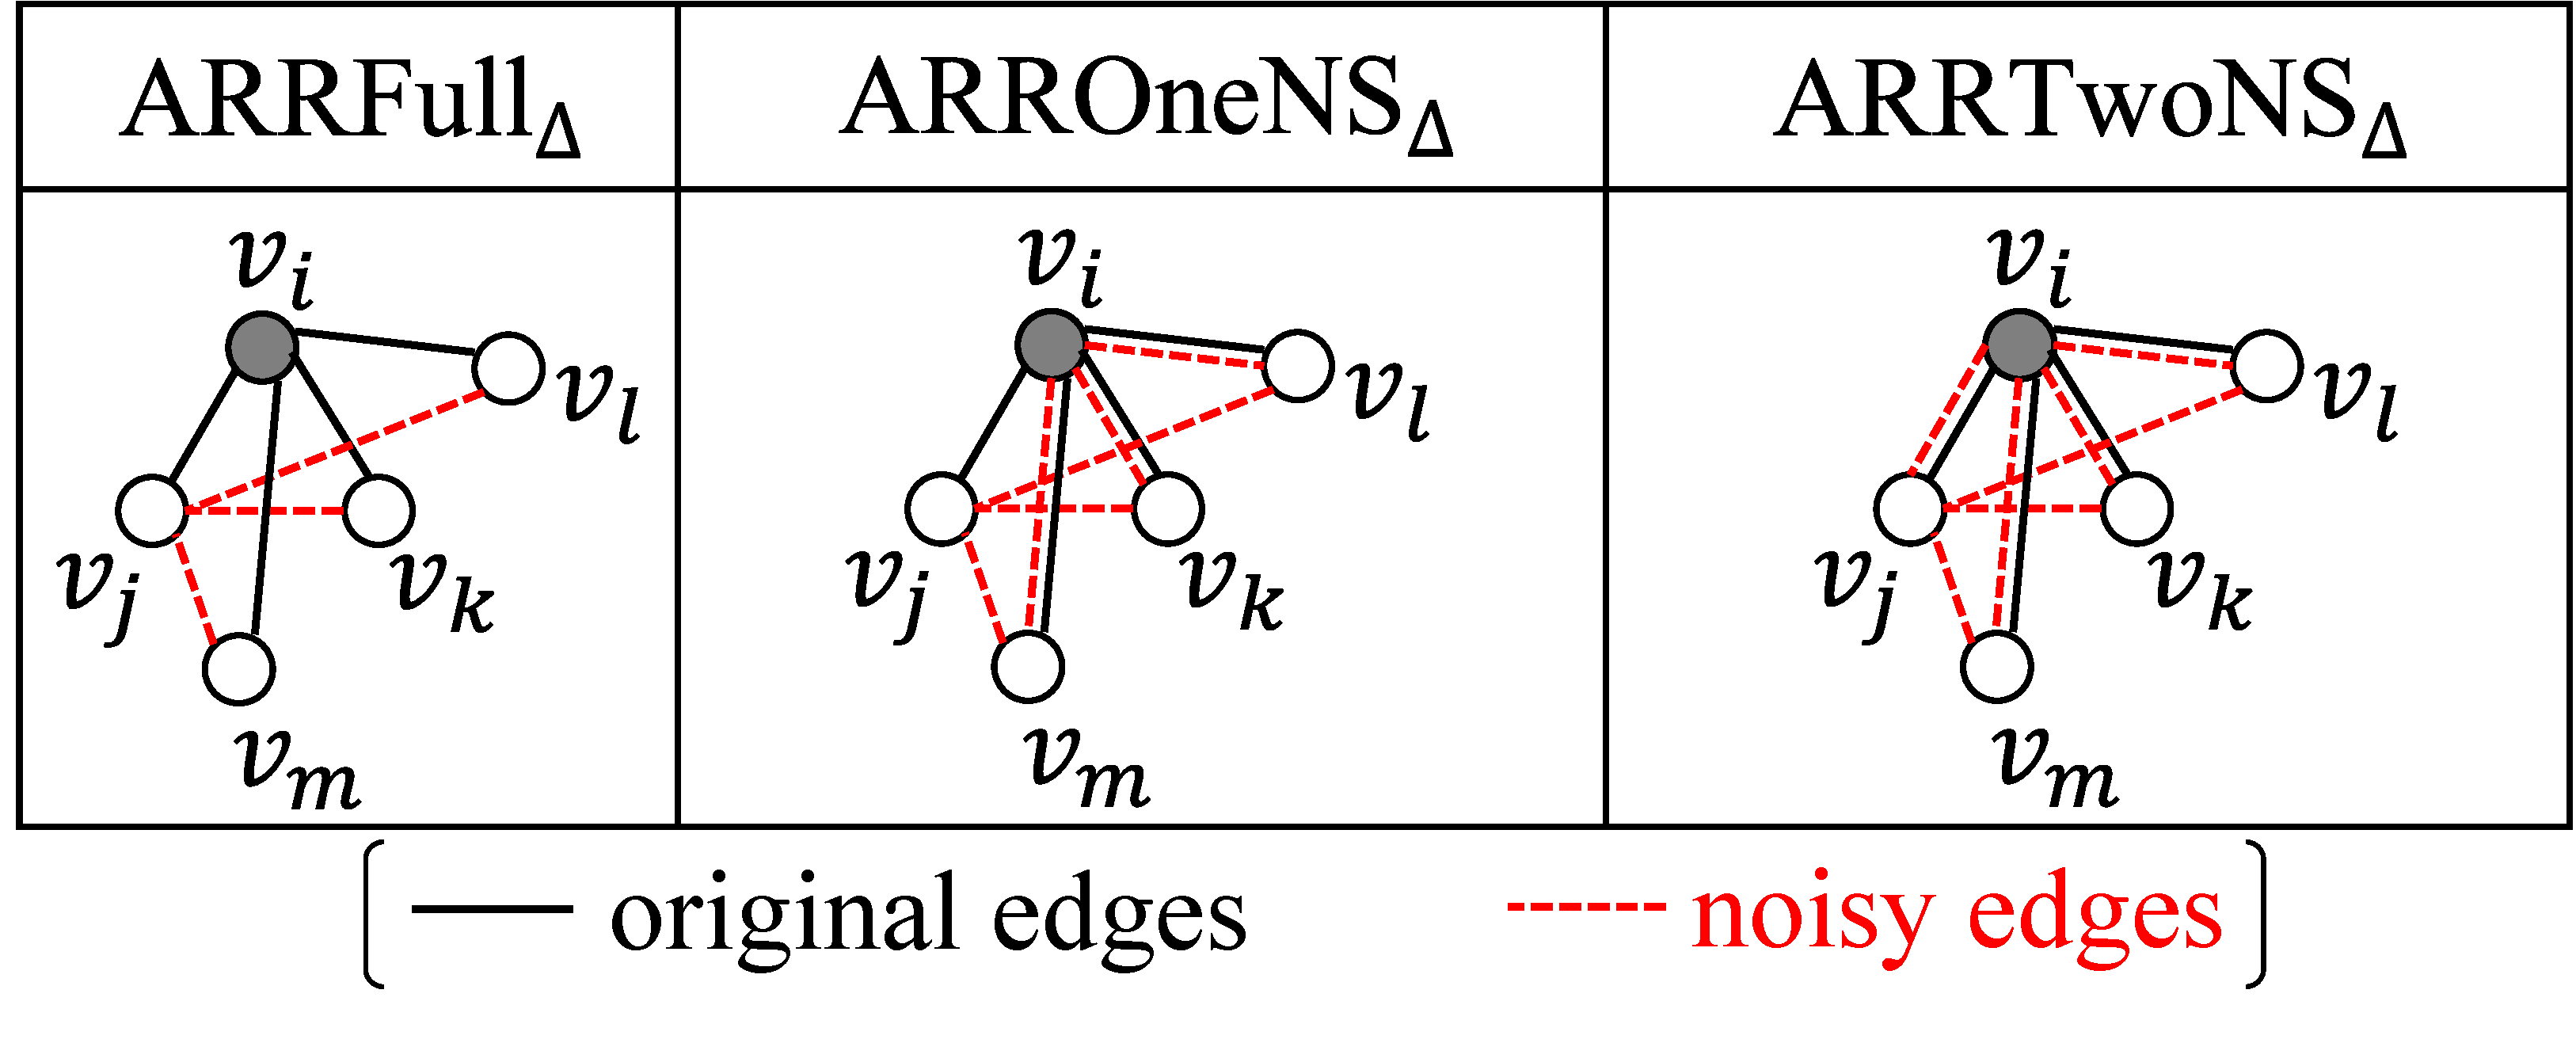
\includegraphics[width=0.78\linewidth]{fig/double_clipping.pdf}
  \vspace{-4mm}
  \caption{Noisy triangles involving edge $(v_i,v_j)$ counted by user $v_i$ ($j<k,l,m<i$).} 
  \label{chap2-fig:reduce_noisy_triangles}
%\end{figure}
\vspace{2mm}
%\begin{figure}[t]
  \centering
  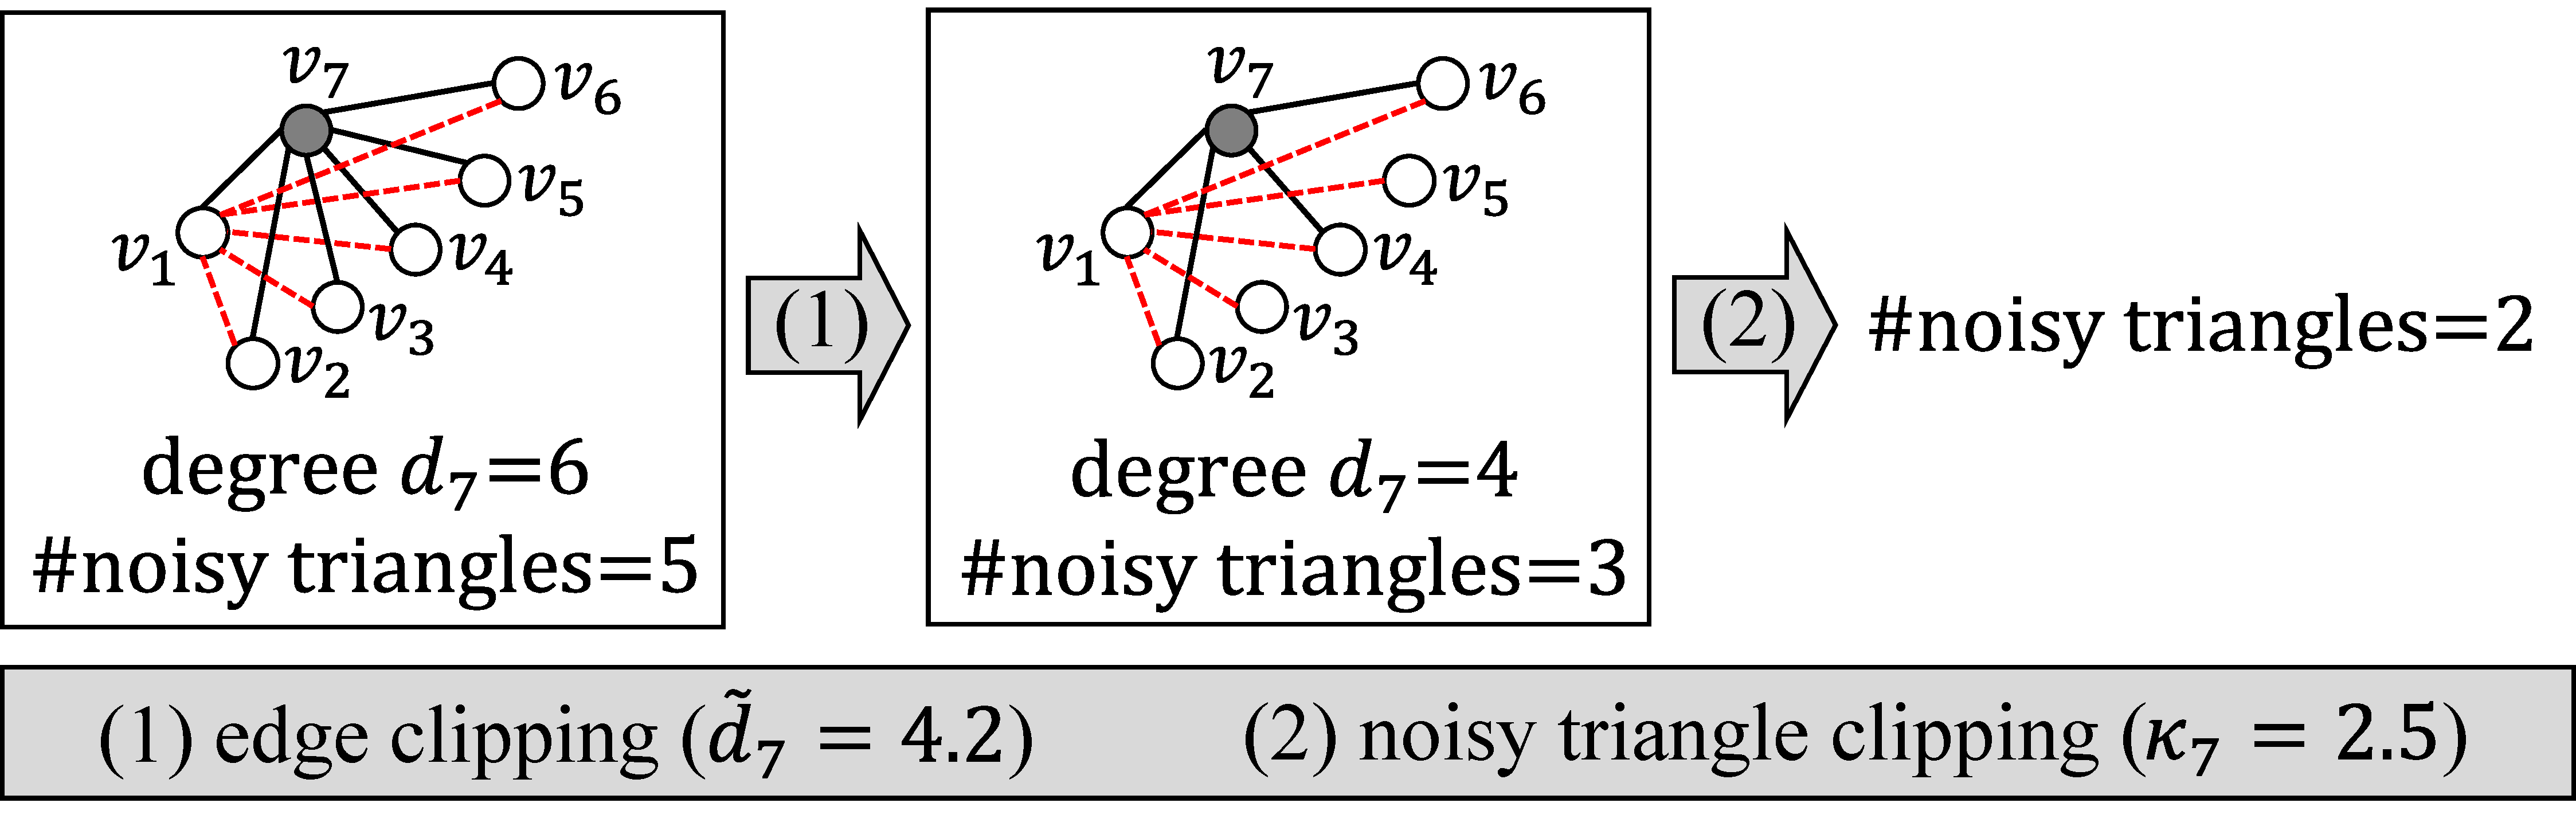
\includegraphics[width=0.99\linewidth]{fig/clip_overview.pdf}
  \vspace{-4mm}
  \caption{Overview of double clipping applied to edge ($v_1,v_7$).} 
  \label{chap2-fig:double-clip_overview}
\end{figure}

% To address the first and second issues explained above, we introduce an edge clipping and triangle clipping, respectively. 
To address these two issues, 
%(i.e., the leakage of $d_i$ and the excess of the noisy triangle count), 
we propose a double clipping technique, which is explained below. 
% which consists of an \textit{adaptive edge clipping} and \textit{noisy triangle clipping}. 

\smallskip
\noindent{\textbf{Algorithm Overview.}}~~Figure~\ref{chap2-fig:double-clip_overview} shows 
% its overview. 
the overview of our double clipping, which consists of an 
% \textit{adaptive edge clipping} 
\textit{edge clipping} 
and \textit{noisy triangle clipping}. 
% The adaptive edge clipping 
The edge clipping 
addresses the first issue (i.e., leakage of $d_i$) 
as follows. 
% by borrowing the idea of adaptive clipping \cite{Andrew_arXiv21,Pichapati_arXiv19} 
% in DP-SGD (Differentially Private Stochastic Gradient Descent). 
% which privately estimates an appropriate clipping threshold in DP-SGD (Stochastic Gradient Descent) \cite{Abadi_CCS16} with DP. 
% Specifically, it 
It privately computes 
a noisy version of 
$d_i$ (denoted by $\td_i$) with edge LDP. 
% Let $\td_i \in \nnreals$ be the private value of $d_i$. 
% user $v_i$ 
% adds the Laplacian noise and some positive constant $\eta \in \nnreals$ to $d_i$ to provide edge LDP 
% and 
Then it 
%performs edge clipping 
%(a.k.a. graph projection \cite{Day_SIGMOD16,Ding_TKDE21,Kasiviswanathan_TCC13,Raskhodnikova_arXiv15}), which 
removes some neighbors from a neighbor list $\bma_i$ so that the degree of $v_i$ never exceeds 
% the private estimate of $d_i$. 
% the private value of $d_i$ 
% (denoted by $\td_i \in \nnreals$). 
% (denoted by $\td_i$). 
the noisy degree $\td_i$. 
This removal process is also known as graph projection \cite{Day_SIGMOD16,Ding_TKDE21,Kasiviswanathan_TCC13,Raskhodnikova_arXiv15}. 
% This kind of technique is called adaptive clipping \cite{Andrew_arXiv21,Pichapati_arXiv19} 
% in DP-SGD (Stochastic Gradient Descent) \cite{Abadi_CCS16} because it privately estimates an appropriate clipping threshold with DP. 
% Adaptive edge clipping 
Edge clipping 
is 
% also 
used in \cite{Imola_USENIX21} to obtain a 
% private value of 
noisy version of 
% the maximum degree 
$d_{max}$. 
%(though ours is to obtain a noisy version of $d_i$). 

% The triangle clipping addresses the second issue (i.e., excess of the noisy triangle count) by reducing the noisy triangle count so that it never exceeds a 
% user-dependent threshold $\kappa_i \in \nnints$. 
The main novelty in our double clipping lies at the \textit{noisy triangle clipping} to address the second issue (i.e., excess of the noisy triangle count). 
% Note that 
This issue appears 
% only 
when 
% each edge is sampled and 
we attempt to reduce the global sensitivity by using 
a very small sampling probability for each edge. 
% value of $\mu$ in the ARR.  
% using a stochastic algorithm such as the ARR. 
Therefore, the noisy triangle clipping has not been studied in the existing works on private triangle counting 
% \cite{Ding_TKDE21,Imola_USENIX21,Karwa_PVLDB11,Kasiviswanathan_TCC13,Song_arXiv18,Sun_CCS19,Ye_ICDE20,Ye_TKDE21,Zhang_SIGMOD15}, 
\cite{Ding_TKDE21,Imola_USENIX21,Karwa_PVLDB11,Kasiviswanathan_TCC13,Sun_CCS19,Ye_ICDE20,Ye_TKDE21,Zhang_SIGMOD15}, 
because they do not apply a sampling technique. 

Our noisy triangle clipping reduces the noisy triangle count so that it never exceeds a 
user-dependent clipping threshold 
$\kappa_i \in \nnreals$. 
% $\kappa_i = \lambda_i \mu^* \td_i$, where $\lambda_i \in \nats$. 
% We call $\kappa_i$ and $\lambda_i$ the \textit{clipping threshold} and \textit{clipping coefficient}, respectively. 
Then a crucial issue is how to set 
an appropriate 
% clipping 
threshold 
$\kappa_i$. 
We theoretically analyze the probability that the noisy triangle count exceeds $\kappa_i$ 
(referred to as the \textit{triangle excess probability}) 
as a function of 
the ARR parameter $\mu$ and the 
% private value $\td_i$ of $d_i$. 
noisy degree $\td_i$. 
% of user $v_i$. 
Then we set $\kappa_i$ so that 
the triangle excess probability 
% the probability 
is very small ($=10^{-6}$ in our experiments). 

We use the clipping threshold $\kappa_i$ as a global sensitivity. 
% of the Laplacian noise. 
Note that $\kappa_i$ provides edge LDP because $\td_i$ provides edge LDP, 
% and $\kappa_i$ depends on only $\mu$ and $\td_i$ 
i.e., immunity to post-processing \cite{DP}. 
$\kappa_i$ is also very small when $\mu \ll 1$, as it is determined based on $\mu$. 

% We also emphasize that our double clipping does \textit{not} assume that $d_{max}$ is public, because it privately computes $\td_i$. 
% by adaptive edge clipping.

\subsection{Algorithms}
\label{chap2-sub:algorithms}
Algorithm~\ref{chap2-alg:clip} shows our double clipping algorithm. 
All the processes are run by user $v_i$ at the second round. 
Thus, there is no interaction with the server in Algorithm~\ref{chap2-alg:clip}.

\setlength{\algomargin}{5mm}
\begin{algorithm}[t]
  \SetAlgoLined
  \KwData{Neighbor list $\bma_i \in \{0,1\}^n$, privacy budget
  $\epsilon_0 \in \nnreals$ 
  $\mu \in [0,\frac{e^{\epsilon_1}}{e^{\epsilon_1} + 1}]$, 
  %$\eta \in \nnreals$.
  $\alpha \in \nnreals$, 
  $\beta \in \nnreals$.
  }
  \KwResult{$\hw_i$.}
  $\mu^* \leftarrow \mu$, $\mu^2$, and $\mu^3$ in F, O, and T, respectively\;
  \tcc{Edge clipping.}
  %$\td_i = \max\{d_i + \Lap(\frac{1}{\epsilon_0}) + \eta$, 0\}\;
  $\td_i = \max\{d_i + \Lap(\frac{1}{\epsilon_0}) + \alpha$, 0\}\;
  \tcc{Remove $d_i - \lfloor \td_i \rfloor$ neighbors if $d_i > \td_i$.}
  $\bma_i \leftarrow \texttt{GraphProjection}(\bma_i, \td_i)$\;
  \tcc{Noisy triangle clipping.}
  \For{$j$ \rm{such that} $a_{i,j} = 1$ \rm{and} $j<i$}{
    $t_{i,j} \leftarrow |\{(v_i,v_j,v_k) : a_{i,k} = 1, (v_j,v_k) \in M_i, j<k<i \}|$\;
  }
%  \tcc{Calculate $\kappa_i$ such that $\kappa_i \in [\mu^* \td_i, \td_i]$.}
   \tcc{Calculate $\kappa_i \in [\mu^* \td_i, \td_i]$ s.t. the triangle excess probability is $\beta$ or less.}
%  \tcc{Calculate $\lambda_i \in \nats$ such that the triangle excess probability is $\beta$ or less.}
  $\kappa_i \leftarrow \texttt{ClippingThreshold}(\mu, \td_i, \beta)$\;
%  $\lambda_i \leftarrow \texttt{ClippingThreshold}(\mu, \td_i, \beta)$\;
%   $\kappa_i \leftarrow \lambda_i \mu^* \td_i$\;
  $t_i \leftarrow \sum_{a_{i,j} = 1, j<i} \min \{t_{i,j}, \kappa_i\}$\;
  $s_i \leftarrow |\{(v_i,v_j,v_k) : a_{i,j} = a_{i,k} = 1, j<k<i\}|$\;
  $w_i \leftarrow t_i - \mu^* \rho s_i$\;
  $\hw_i \leftarrow w_i + \Lap(\frac{\kappa_i}{\epsilon_2})$\;
  \KwRet{$\hw_i$}
  \caption{Our double clipping algorithm. 
  ``F'', ``O'', ``T'' are shorthands for 
  \AlgOne{}, \AlgTwo{}, and \AlgThree{}, respectively.
  All the processes are run by user $v_i$.
  }\label{chap2-alg:clip}
\end{algorithm}

\smallskip
\noindent{\textbf{Edge Clipping.}}~~The edge clipping appears in lines 2-3 of Algorithm~\ref{chap2-alg:clip}. 
It uses a privacy budget $\epsilon_0 \in \nnreals$. 
% for privately computing $d_i$. 

In line 2, user $v_i$ adds the Laplacian noise $\Lap(\frac{1}{\epsilon_0})$ to her degree $d_i$. 
Since adding/removing one edge changes $d_i$ by at most $1$, this process provides $\epsilon_0$-edge LDP. 
$v_i$ also adds some non-negative constant 
% $\eta \in \nnreals$ 
$\alpha \in \nnreals$ 
to $d_i$. 
We add this value so that edge removal (in line 3) occurs with a very small probability; 
e.g., in our experiments, we set $\alpha = 150$, where 
% when $\epsilon_0 = 0.1$ and $\alpha = 150$, 
edge removal occurs with probability $1.5 \times 10^{-7}$ when $\epsilon_0 = 0.1$. 
A similar technique is introduced in \cite{Sun_CCS19} to provide ($\epsilon, \delta)$-DP \cite{DP} with small $\delta$. 
The difference between ours and \cite{Sun_CCS19} is that we perform edge clipping 
% (graph projection) 
to always provide $\epsilon$-DP; i.e., $\delta = 0$.
Let $\td_i \in \nnreals$ be the noisy degree of $v_i$.

In line 3, user $v_i$ calls the function \texttt{GraphProjection}, which performs graph projection as follows; 
if $d_i > \td_i$, randomly remove $d_i - \lfloor \td_i \rfloor$ neighbors from $\bma_i$; otherwise, do nothing. 
Consequently, the degree 
% $d_i$ 
of $v_i$ never exceeds $\td_i$. 

\begin{table*}[t]
  \centering
  \begin{tabular}{|l|c|c|c|}
    \hline
    & \AlgOne & \AlgTwo & \AlgThree \\ \hline
    Privacy 
    & \multicolumn{3}{|c|}{$(\epsilon_0 + \epsilon_1 + \epsilon_2)$-edge LDP and $(\epsilon_0 + \epsilon_1 + \epsilon_2)$-relationship DP} \\ \hline
    %& $\epsilon_0 + \epsilon_1 + \epsilon_2$ & $\epsilon_0 + \epsilon_1 + \epsilon_2$ &
    %$\epsilon_0 + \epsilon_1 + \epsilon_2$ \\ \hline
    Expected $l_2$ loss 
    % & $\frac{2 C_4(G) + S_2(G)}{\mu(1-e^{-\epsilon_1})^2}$ + $\frac{2 \sum_{i=1}^n \kappa_{i}^2}{\mu^2 (1-e^{-\epsilon_1})^2 \epsilon_2^2}$
    % & $O\left(\frac{n d_{max}^3}{\mu(1-e^{-\epsilon_1})^2} + \frac{2 \sum_{i=1}^n \lambda_{i}^2 \td_i^2}{(1-e^{-\epsilon_1})^2 \epsilon_2^2}\right)$
    & $O\left(\frac{n d_{max}^3}{\mu(1-e^{-\epsilon_1})^2} + \frac{2 \sum_{i=1}^n \kappa_{i}^2}{\mu^2(1-e^{-\epsilon_1})^2 \epsilon_2^2}\right)$
    % & $\frac{\mu(12 S_3(G) + 6 P_3(G)) + 6 S_2(G)}{\mu^2(1-e^{-\epsilon_1})^2}$ + $\frac{2 \sum_{i=1}^n \kappa_{i}^2}{\mu^4 (1-e^{-\epsilon_1})^2 \epsilon_2^2}$
    % & $O\left(\frac{n d_{max}^2}{\mu^2(1-e^{-\epsilon_1})^2} + \frac{2 \sum_{i=1}^n \lambda_{i}^2 \td_i^2}{(1-e^{-\epsilon_1})^2 \epsilon_2^2} \right)$
    & $O\left(\frac{n d_{max}^2}{\mu^2(1-e^{-\epsilon_1})^2} + \frac{2 \sum_{i=1}^n \kappa_{i}^2}{\mu^4 (1-e^{-\epsilon_1})^2 \epsilon_2^2} \right)$
    % & $\frac{\mu^2 (12 S_3(G) + 6 P_3(G)) + 6 S_2(G)}{\mu^3(1-e^{-\epsilon_1})^2}$ + $\frac{2 \sum_{i=1}^n \kappa_{i}^2}{\mu^6 (1-e^{-\epsilon_1})^2 \epsilon_2^2}$ \\ \hline
    % & $O\left(\frac{n d_{max}^2}{\mu^3(1-e^{-\epsilon_1})^2} + \frac{2 \sum_{i=1}^n \lambda_{i}^2 \td_i^2}{(1-e^{-\epsilon_1})^2 \epsilon_2^2} \right)$ \\ \hline
    & $O\left(\frac{n d_{max}^2}{\mu^3(1-e^{-\epsilon_1})^2} + \frac{2 \sum_{i=1}^n \kappa_{i}^2}{\mu^6 (1-e^{-\epsilon_1})^2 \epsilon_2^2} \right)$ \\ \hline
    % $l_2$ loss of emp 
    % & $\frac{2 C_4(G) + S_2(G)}{\mu_F(1-e^{-\epsilon_1})^2}$
    % & $\frac{\mu_O(12 S_3(G) + 6 P_3(G)) + 6 S_2}{\mu_O^2(1-e^{-\epsilon_1})^2}$
    % & $\frac{\mu_T^2 (12 S_3(G) + 6 P_3(G)) + 6 S_2}{\mu_T^3(1-e^{-\epsilon_1})^2}$ \\ \hline
    % $l_2$ loss of \Lap{} 
    % & $\frac{2 \sum_{i=1}^n \kappa_{i,F}^2}{\mu_F^2 (1-e^{-\epsilon_1})^2 \epsilon_2^2}$
    % & $\frac{2 \sum_{i=1}^n \kappa_{i,O}^2}{\mu_F^2 (1-e^{-\epsilon_1})^2 \epsilon_2^2}$
    % & $\frac{2 \sum_{i=1}^n \kappa_{i,T}^2}{\mu_F^2 (1-e^{-\epsilon_1})^2 \epsilon_2^2}$ \\ \hline
    $\text{Cost}_{DL}$ & 
    $\mu n^2 \log n$ 
    % $\mu e^{-\epsilon_1} n^2 \log n$ 
    % $\mu_F e^{-\epsilon_1} n(n-1) \log n$ 
    % $(n(n-1) \mu_F \rho + |E| \mu_F (1 - \rho)) \log n$ 
    & 
    $\mu^2 n^2 \log n$ 
    % $\mu^2 e^{-\epsilon_1} n^2 \log n$ 
    % $\mu_O^2 e^{-\epsilon_1} n(n-1) \log n$ 
    & 
    $\mu^3 n^2 \log n$ 
    % $\mu^3 e^{-\epsilon_1} n^2 \log n$ 
    % $\mu_T^3 e^{-\epsilon_1} n(n-1) \log n$ 
    \\ \hline
    $\text{Cost}_{UL}$ & 
    $\mu n \log n$ & $\mu n \log n$ & $\mu n \log n$ 
    % $\mu e^{-\epsilon_1} n \log n$ & $\mu e^{-\epsilon_1} n \log n$ & $\mu e^{-\epsilon_1} n \log n$ 
    \\ \hline
  \end{tabular}
  \vspace{-2mm}
  \caption{Performance guarantees 
  %Privacy, expected $l_2$ loss, and download/upload cost 
  of our three algorithms with double clipping when the edge removal and triangle removal do not occur. 
  %($C_4$: \#$4$-cycles, $P_3$: \#$3$-paths, $S_k$: \#$k$-stars). 
  %($\lambda_i$: clipping coefficient, $\td_i$: noisy degree).
  The expected $l_2$ loss assumes that $\mu$ is small. 
  The download (resp.~upload) cost is an upper-bound in (\ref{chap2-eq:CostDL_F}) 
  %, (\ref{chap2-eq:CostDL_O}), (\ref{chap2-eq:CostDL_T}), 
  (resp.~(\ref{chap2-eq:CostUL_proposal})).
  %approximation when $d_{max} \ll n$. 
  %the graph $G$ is sparse.
  }
  \label{chap2-tab:privacy_utility_cost}
\end{table*}

\smallskip
\noindent{\textbf{Noisy Triangle Clipping.}}~~The noisy triangle clipping appears in lines 4-11 of Algorithm~\ref{chap2-alg:clip}. 

% First, 
In lines 4-6, 
user $v_i$ calculates the number $t_{i,j} \in \nnints$ of noisy triangles ($v_i, v_j, v_k$) ($j<k<i$) involving $(v_i,v_j)$ 
(as shown in Figure~\ref{chap2-fig:reduce_noisy_triangles}). 
%such that only one edge ($v_j, v_k$) is noisy 
% for her neighbor $v_j$. 
% (lines 4-6). 
Note that the total number $t_i$ of noisy triangles of $v_i$ can be expressed as: 
$t_i = \sum_{a_{i,j}=1, j<i} t_{i,j}$. 
In line 7, $v_i$ calls the function \texttt{ClippingThreshold}, which calculates a clipping threshold 
% $\kappa_i$ 
$\kappa_i \in [\mu^* \td_i, \td_i]$ 
($\mu^* = \mu$, $\mu^2$, and $\mu^3$ in 
``F'', ``O'', and ``T'', respectively) 
based on the ARR parameter $\mu$ and the noisy degree $\td_i$ so that 
% $\kappa_i \in [\mu^* \td_i, \td_i]$ 
% ($\mu^* = \mu$, $\mu^2$, and $\mu^3$ in 
% ``F'', ``O'', and ``T'', respectively) 
% and 
the triangle excess probability does not exceed some constant $\beta \in \nnreals$. 
% $\kappa_i$ takes a value between $\mu^* \td_i$ and $\td_i$; i.e., $\kappa_i \in [\mu^* \td_i, \td_i]$. 
We explain how to calculate 
% $\kappa_i$ from $\mu$ and $\td_i$ 
the triangle excess probability 
in Section~\ref{chap2-sub:clip_theoretical_analysis}. 
% in detail. 
In line 8, $v_i$ calculates the total number $t_i$ of noisy triangles by summing up $t_{i,j}$, with the exception that $v_i$ adds $\kappa_i$ 
%(rather than $t_{i,j}$) 
if $t_{i,j} > \kappa_i$. 
%$t_{i,j}$ exceeds $\kappa_i$. 
In other words, triangle removal occurs 
% when 
if 
$t_{i,j} > \kappa_i$. 
% Consequently, 
Then, 
the number 
% $t_{i,j}$ 
of noisy triangles involving $(v_i,v_j)$ never exceeds $\kappa_i$. 

Lines 9-11 in Algorithm~\ref{chap2-alg:clip} are the same as lines 12-14 in Algorithm~\ref{chap2-alg:unify}, except that 
the global sensitivity in the former (resp.~latter) is $\kappa_i$ (resp.~$d_{max}$). 
% the global sensitivity in Algorithm~\ref{chap2-alg:clip} is $\kappa_i$. 
Line 11 in Algorithm~\ref{chap2-alg:clip} provides $\epsilon_2$-edge LDP because the number of triangles involving $(v_i,v_j)$ is now upper-bounded by $\kappa_i$. 

\smallskip
\noindent{\textbf{Our Entire Algorithms with Double Clipping.}}~~We can run our algorithms \AlgOne{}, \AlgTwo{}, \AlgThree{} with double clipping just by replacing lines 11-14 in Algorithm~\ref{chap2-alg:unify} with lines 2-11 in Algorithm~\ref{chap2-alg:clip}. 
That is, after calculating $\hw_i$ by Algorithm~\ref{chap2-alg:clip}, $v_i$ uploads $\hw_i$ to the server. 
Then the server calculates an estimate of $f_\triangle(G)$ as $\hf_\triangle(G) = \frac{1}{\mu^*(1-\rho)}\sum_{i=1}^n \hw_i$. 
%as in line 17 of Algorithm~\ref{chap2-alg:unify}. 
% where $\mu^* = \mu$, $\mu^2$, and $\mu^3$ in 
% ``F'', ``O'', and ``T'', respectively). 

We also note that the input $d_{max}$ in Algorithm~\ref{chap2-alg:unify} is no longer necessary thanks to the edge clipping; i.e., our entire algorithms with double clipping do not assume that $d_{max}$ is public. 
% , because $v_i$ privately calculates $d_i$ by edge clipping.

\subsection{Theoretical Analysis}
\label{chap2-sub:clip_theoretical_analysis}
% \paragraph{Privacy}
% \smallskip
We now perform a theoretical analysis on the privacy and utility of our double clipping. 
% All the proofs appear in \arxiv{Appendix~\ref{chap2-sec:proof_double_clip}}\conference{the full version \cite{Imola_arXiv22}}. 

\smallskip
\noindent{\textbf{Privacy.}}~~We begin with the privacy guarantees:
% Our algorithms with double clipping have the following privacy guarantees:
\begin{theorem}\label{chap2-thm:privacy_DC}
  For $i \in [n]$, 
  let $\calR_i^1, \calR_i^2(M_i)$ be the randomizers used by user $v_i$ in
  rounds $1$ and $2$ of our algorithms with double clipping (Algorithms~\ref{chap2-alg:unify} and \ref{chap2-alg:clip}). 
  Let $\calR_i(\bma_i) = (\calR_i^1(\bma_i), \calR_i^2(M_i)(\bma_i))$ 
  be the composition of the two randomizers. 
  Then,
  $\calR_i$ satisfies $(\epsilon_0 + \epsilon_1 + \epsilon_2)$-edge LDP, 
  %for $i \in [n]$, 
  and $(\calR_1,
  \ldots, \calR_n)$ satisfies $(\epsilon_0 + \epsilon_1 + \epsilon_2)$-relationship DP.
\end{theorem}

\smallskip
\noindent{\textbf{Utility.}}~~Next, we show the triangle excess probability: 
% the probability that the noisy triangle count $t_{i,j}$ exceeds $\kappa_i$:

\begin{theorem}\label{chap2-thm:triangle_excess}
%Let $\mu^* = \mu_F$ and $\mu_O^2$ in \AlgOne{} and \AlgTwo{}, respectively. 
%In \AlgOne{} and \AlgTwo{}, 
%In \AlgOne{}, \AlgTwo{}, \AlgThree{}, 
% Let $\mu_F, \mu_O, \mu_T \in [0,\frac{e^{\epsilon}}{e^{\epsilon_1} + 1}]$. 
% For $i \in [n]$, let $\td_i \in \nnreals$ be a noisy degree of user $v_i$ output by edge clipping. 
% Let $\kappa_i$
In Algorithm~\ref{chap2-alg:clip}, the triangle excess probability (i.e., probability that the number of noisy triangles $t_{i,j}$ involving edge $(v_i, v_j)$ exceeds a clipping threshold $\kappa_i$) is:
  \begin{align}
    \hspace{-1mm} \Pr(t_{i,j} > \kappa_i) &\leq \textstyle{\exp \left[-\td_i D \left(\frac{\kappa_i}{\td_i} \parallel \mu \right) \right]} \label{chap2-eq:AlgI_clip_bound} \\
    \hspace{-1mm} \Pr(t_{i,j} > \kappa_i) &\leq \textstyle{\exp \left[-\td_i D \left(\frac{\kappa_i}{\td_i} \parallel \mu^2 \right) \right]} \label{chap2-eq:AlgII_clip_bound}\\
%   \end{align}
%   \begin{align}
    \hspace{-1mm} \Pr(t_{i,j} > \kappa_i) &\leq 
    \textstyle{\mu \exp \left[-\td_i D \left(\frac{\max\{\kappa_i,\mu^2 \td_i\}}{\td_i} \parallel \mu^2 \right) \right]}
    % \begin{cases}
    %     \mu_T \exp \left[-\td_i D \left(\frac{\kappa_i}{\td_i} \parallel \mu_T^2 \right) \right]   &   \mathrm{(if}~ \kappa_i \geq \mu_T^2 \td_i)\\
    %     \mu_T   &   \mathrm{(if}~ \mu_T^3 \td_i \leq \kappa_i < \mu_T^2 \td_i),
    % \end{cases}
    \label{chap2-eq:AlgIII_clip_bound}
  \end{align}
  in \AlgOne{}, \AlgTwo{}, and \AlgThree{}, respectively, 
  where 
  % $\mu^* = \mu_F$ and $\mu_O^2$ in \AlgOne{} and \AlgTwo{}, respectively, and 
  $D(p_1 \parallel p_2)$ is the Kullback-Leibler divergence between two Bernoulli distributions; i.e., 
  %$D(p_1 \parallel p_2) = p_1 \log \frac{p_1}{p_2} + (1-p_1) \log \frac{1-p_1}{1-p_2}$.
  %with $p_1$ and $p_2$:
  %the Bernoulli($p_1$) and Bernoulli($p_2$) distribution; 
\begin{align*}
    \textstyle{D(p_1 \parallel p_2) = p_1 \log \frac{p_1}{p_2} + (1-p_1) \log \frac{1-p_1}{1-p_2}.}
\end{align*}
\end{theorem}
In all of (\ref{chap2-eq:AlgI_clip_bound}), (\ref{chap2-eq:AlgII_clip_bound}), and (\ref{chap2-eq:AlgIII_clip_bound}), we use the Chernoff bound, which is known to be reasonably tight \cite{Arratia_BMB89}. 

\smallskip
\noindent{\textbf{Setting $\kappa_i$.}}~~The function \texttt{ClippingThreshold} in Algorithm~\ref{chap2-alg:clip} sets a clipping threshold $\kappa_i$ of user $v_i$ based on Theorem~\ref{chap2-thm:triangle_excess}. 
Specifically, we set $\kappa_i = \lambda_i \mu^* \td_i$, where $\lambda_i \in \nats$, and calculate $\lambda_i$ as follows. 
We initially set $\lambda_i = 1$ and keep increasing $\lambda_i$ by $1$ 
% initially set $\kappa_i = \mu^* \td_i$ and keep increasing $\kappa_i$ by $\mu^* \td_i$ 
until the upper-bound (i.e., right-hand side of (\ref{chap2-eq:AlgI_clip_bound}), (\ref{chap2-eq:AlgII_clip_bound}), or (\ref{chap2-eq:AlgIII_clip_bound})) is smaller than or equal to the triangle excess probability $\beta$. 
In our experiments, we set $\beta = 10^{-6}$. 
% We call $\lambda_i$ the \textit{clipping coefficient} of $v_i$. 

\smallskip
\noindent{\textbf{Large $\kappa_i$ of \AlgThree{}.}}~~By 
% In our experiments, we set $\mu$ so that $\mu$ in \AlgOne{} is equal to $\mu^2$ in \AlgTwo{} and also equal to $\mu^3$ in \AlgThree{}. 
% Then by 
(\ref{chap2-eq:AlgI_clip_bound}) and (\ref{chap2-eq:AlgII_clip_bound}), the upper-bound on the triangle excess probability is the same between \AlgOne{} and \AlgTwo{}. 
% However, 
In contrast, 
\AlgThree{} has a larger upper-bound. 
For example, 
when $\kappa_i = 15 \mu^* \td_i$, $\mu^* = 10^{-3}$, and $\td_i=1000$, 
the right-hand sides of (\ref{chap2-eq:AlgI_clip_bound}), (\ref{chap2-eq:AlgII_clip_bound}), and (\ref{chap2-eq:AlgIII_clip_bound}) are $2.5 \times 10^{-12}$, $2.5 \times 10^{-12}$, and $3.3 \times 10^{-2}$, respectively. 
Consequently, \AlgThree{} has a larger global sensitivity $\kappa_i$ for the same value of $\beta$.

% \smallskip
% \noindent{\textbf{\AlgTwo{} vs. \AlgThree{}.}}~~Now we explain the reason that \AlgTwo can reduce the global sensitivity more effectively than \AlgThree (as described in Section~\ref{chap2-sub:algorithms_overview}).  
% using Figure~\ref{chap2-fig:reduce_noisy_triangles}. 
% As with \AlgOne, 
We can explain a large global sensitivity $\kappa_i$ of \AlgThree{} as follows. 
The number $t_{i,j}$ of noisy triangles involving $(v_i,v_j)$ in 
\AlgOne{} is expected to be around $\mu d_i$ because one noisy edge is in each noisy triangle (as in Figure~\ref{chap2-fig:reduce_noisy_triangles}) and all noisy edges are independent. 
For the same reason, $t_{i,j}$ in \AlgTwo{} is expected to be around $\mu^2 d_i$.  
% \AlgTwo{} is expected to be around $\mu_O^2 d_i$ because two noisy edges are in each noisy triangle (as in Figure~\ref{chap2-fig:reduce_noisy_triangles}) and all noisy edges are independent. 
% 
However, 
% the number of noisy triangles involving $(v_i,v_j)$ 
$t_{i,j}$ in \AlgThree{} is \textit{not} expected to be around $\mu^3 d_i$, because all the noisy triangles have noisy edge $(v_i,v_j)$ in common (as in Figure~\ref{chap2-fig:reduce_noisy_triangles}). 
Then, 
% the expected noisy triangle count 
the expectation of $t_{i,j}$ 
largely depends on the presence/absence of the noisy edge $(v_i,v_j)$; i.e., if noisy edge $(v_i,v_j)$ exists, 
it is $\mu^2 d_i$; otherwise, $0$. 
% Consequently, 
% the noisy triangle count (i.e., global sensitivity) 
% the global sensitivity 
Thus, 
$\kappa_i$ 
cannot be effectively reduced by double clipping. 
% Section~\ref{chap2-sub:clip_theoretical_analysis} shows a more formal result on this. 

\smallskip
\noindent{\textbf{Summary.}}~~The 
% privacy, expected $l_2$ loss, download/upload cost 
performance guarantees 
of our three algorithms with double clipping can be summarized in Table~\ref{chap2-tab:privacy_utility_cost}.

% The expected $l_2$ loss can be expressed $O(n d_{max}^3)$, $O(n d_{max}^2)$, and $O(n d_{max}^2)$, 
% For the $l_2$ loss, 
The first and second terms of the expected 
$l_2$ loss are the $l_2$ loss of empirical estimation and that of the Laplacian noise, respectively. 
For small 
% $\mu_F$ ($=\mu_O^2 = \mu_T^3$), 
$\mu$, 
the $l_2$ loss of empirical estimation can be expressed as $O(n d_{max}^3)$, $O(n d_{max}^2)$, and $O(n d_{max}^2)$ in \AlgOne{}, \AlgTwo{}, \AlgThree{}, respectively, as explained in Section~\ref{chap2-sub:algorithms_theoretical_analysis}. 
% (when we regard $\epsilon_1$ and $\epsilon_2$ as constants). 
% The large $l_2$ loss of \AlgOne{} is caused by the number $C_4$ of $4$-cycles that is written as $O(n d_{max}^3)$. 
The $l_2$ loss of the Laplacian noise is 
$O(\sum_{i=1}^n \kappa_i^2)$, 
% $O(\sum_{i=1}^n \lambda_i^2 \td_i^2)$, 
which is much smaller than $O(n d_{max}^2)$. 
% when $\lambda_i$ is small. 
Thus, our \AlgTwo{} that effectively reduces $\kappa_i$ provides the smallest error, 
% for a large graph or dense graph where $C_4$ is large, 
as shown in our experiments.

We also note that 
both the space and the time complexity to compute and send $M_i$ in our algorithms 
% time and space complexity of 
% our algorithms at the server side 
are $O(\mu^* n^2)$ (as $|E'| =  O(\mu^* n^2)$), which is much smaller than \cite{Imola_USENIX21} ($=O(n^2)$). 


\section{Experiments}
\label{chap2-sec:experiments}

% Based on the theoretical results in Sections~\ref{chap2-sub:algorithms_theoretical_analysis} and \ref{chap2-sub:clip_theoretical_analysis}, we would like to pose the following questions:
To evaluate each component of our algorithms in Sections~\ref{chap2-sec:algorithms} and \ref{chap2-sec:double_clip} as well as our entire algorithms (i.e., \AlgOne, \AlgTwo, \AlgThree with double clipping), we pose the following three research questions:
%\begin{enumerate}
\begin{description}[leftmargin=9.75mm]
% \begin{itemize}[leftmargin=9.7mm]
    \item[RQ1.] 
    %\item 
    How do our three triangle counting algorithms 
    (i.e., \AlgOne, \AlgTwo, \AlgThree) in Section~\ref{chap2-sec:algorithms} compare with each other in terms of accuracy?
    \item[RQ2.] 
    %\item 
    How much does our double clipping technique in Section~\ref{chap2-sec:double_clip} decrease the estimation error?
    %increases the utility?
    \item[RQ3.] 
    %\item 
    How much do our entire algorithms reduce the communication cost, compared to the existing algorithm~\cite{Imola_USENIX21}, while keeping high utility (e.g., relative error $\ll 1$)?
% \end{enumerate}
\end{description}
% \end{itemize}
% To answer to the questions, we designed our experiments.
% We explain our experimental setup in Section~\ref{chap2-sub:setup}. 
% Note that we compare our entire algorithms with the two-rounds algorithm~\cite{Imola_USENIX21} 
% because one-round algorithms result in a very large estimation error, as shown in Appendix~\ref{chap2-sec:one-round}. 
% See Appendix~\ref{chap2-sec:one-round} for the comparison with one-round algorithms.
In Appendix~\ref{chap2-sec:one-round}, we also compare our entire algorithms with one-round algorithms.


% focus on the two-rounds algorithms in our experiments. 
% Below we explain our experimental set-up (Section~\ref{chap2-sub:setup}) and report results (Section~\ref{chap2-sub:results}) to answer to the three questions.

\subsection{Experimental Set-up}
\label{chap2-sub:setup}
In our experiments, we used two real graph datasets:

\smallskip
\noindent{\textbf{Gplus.}}~~The Google+ dataset~\cite{McAuley_NIPS12} (denoted by \GPlus{}) 
% includes a social graph collected from users who had shared circles. 
was collected from users who had shared circles. 
% includes publicly available network information collected from users who had shared circles. 
% ego-networks that represent Google+ users who had shared circles and whose network information is publicly available. 
From the dataset, we 
% extracted 
constructed 
a social graph $G=(V,E)$ with $107614$ nodes (users) and $12238285$ edges, where 
% an edge represents that a user follows or is followed by another one. 
edge $(v_i,v_j) \in E$ represents that $v_i$ follows or is followed by $v_j$. 
The average (resp.~maximum) degree in $G$ is $113.7$ (resp.~$20127$). 

\smallskip
\noindent{\textbf{IMDB.}}~~The IMDB (Internet Movie Database)~\cite{IMDB_GD05} (denoted by \IMDB{}) includes a bipartite graph between $896308$ actors and $428440$ movies. 
From this, we constructed a graph $G=(V,E)$ with $896308$ nodes (actors) and $57064358$ edges, where edge $(v_i,v_j) \in E$ represents that $v_i$ and $v_j$ have played in the same movie. 
The average (resp.~maximum) degree in $G$ is $63.7$ (resp.~$15451$). 
Thus, \IMDB{} is more sparse than \GPlus{}. 

\smallskip
In \conference{the full version \cite{Imola_arXiv22}}\arxiv{Appendix~\ref{chap2-sec:BAmodel}}, we also evaluate our algorithms using a synthetic graph based on the Barab\'{a}si-Albert model~\cite{NetworkScience}, which has a power-law degree distribution. 
%We report the results in 
%\conference{the full version \cite{Imola_arXiv22}}\arxiv{Appendix~\ref{chap2-sec:BAmodel}}.

% In our three triangle counting algorithms, we set 
% the ARR parameter $\mu$ so that $\mu$ in \AlgOne{} is equal to $\mu^2$ in \AlgTwo{} and also equal to $\mu^3$ in \AlgThree{}; i.e., $\CostDL{}$ is the same between the three algorithms. 
% Let $\mu^* = \mu$, $\mu^2$, and $\mu^3$ in \AlgOne{}, \AlgTwo{}, and \AlgThree{}, respectively. 
We evaluated our algorithms while changing $\mu^*$, where $\mu^* = \mu$, $\mu^2$, and $\mu^3$ in \AlgOne{}, \AlgTwo{}, and \AlgThree{}, respectively. 
$\CostDL{}$ is the same between the three algorithms. 
We typically 
set the total privacy budget $\epsilon$ to $\epsilon=1$ 
% or $2$ 
(at most $2$) 
because it is acceptable in many practical scenarios \cite{DP_Li}. 

In our double clipping, we set $\alpha = 150$ and $\beta = 10^{-6}$ so that both edge removal and triangle removal occur with a very small probability ($\leq 10^{-6}$ when $\epsilon_0 = 0.1$). 
% \commentT{Will write how to set $\td_i$ and $\kappa_i$ in double clipping.}
Then for each algorithm, we evaluated the relative error between the true triangle count $f_\triangle(G)$ and its estimate $\hf_\triangle(G)$. 
% (as described in Section~\ref{chap2-sub:LDP}). 
Since the estimate $\hf_\triangle(G)$ varies depending on the randomness of LDP mechanisms, we ran each algorithm $\tau \in \nats$ times ($\tau=20$ and $10$ for \GPlus{} and \IMDB{}, respectively) and averaged the relative error over the $\tau$ cases.

\subsection{Experimental Results}
\label{chap2-sub:results}

\smallskip
% \noindent{\textbf{Three Algorithms w/ Lap.}}~~
\noindent{\textbf{Performance Comparison.}}~~First, 
we 
% evaluated our algorithms with the Laplacian noise at the second round. 
evaluated our algorithms with the Laplacian noise. 
% and compared them with the existing two-rounds algorithm in \cite{Imola_USENIX21}. 
Specifically, we evaluated all possible combinations of our three algorithms with and without our double clipping (six combinations in total) and compared them with 
the existing two-rounds algorithm in~\cite{Imola_USENIX21}.  
% the algorithm in~\cite{Imola_USENIX21}.  
For algorithms with double clipping, we divided the total privacy budget $\epsilon$ as: 
% used $\frac{\epsilon}{10}$ for the adaptive edge clipping, and the remaining budget 
% $\epsilon_0: \epsilon_1: \epsilon_2 = 0.1: 0.45: 0.45$.
$\epsilon_0 = \frac{\epsilon}{10}$ and 
$\epsilon_1 = \epsilon_2 = \frac{9\epsilon}{20}$. 
Here, we set a very small budget ($\epsilon_0 = \frac{\epsilon}{10}$) for edge clipping because the degree has a small sensitivity (sensitivity$=1$). 
For algorithms without double clipping, we divided $\epsilon$ as $\epsilon_1 = \epsilon_2 = \frac{\epsilon}{2}$ and 
used the maximum degree $d_{max}$ as the global sensitivity. 
% We emphasize again that our algorithms with double clipping do not assume that $d_{max}$ is public.

\begin{figure}[t]
  \centering
  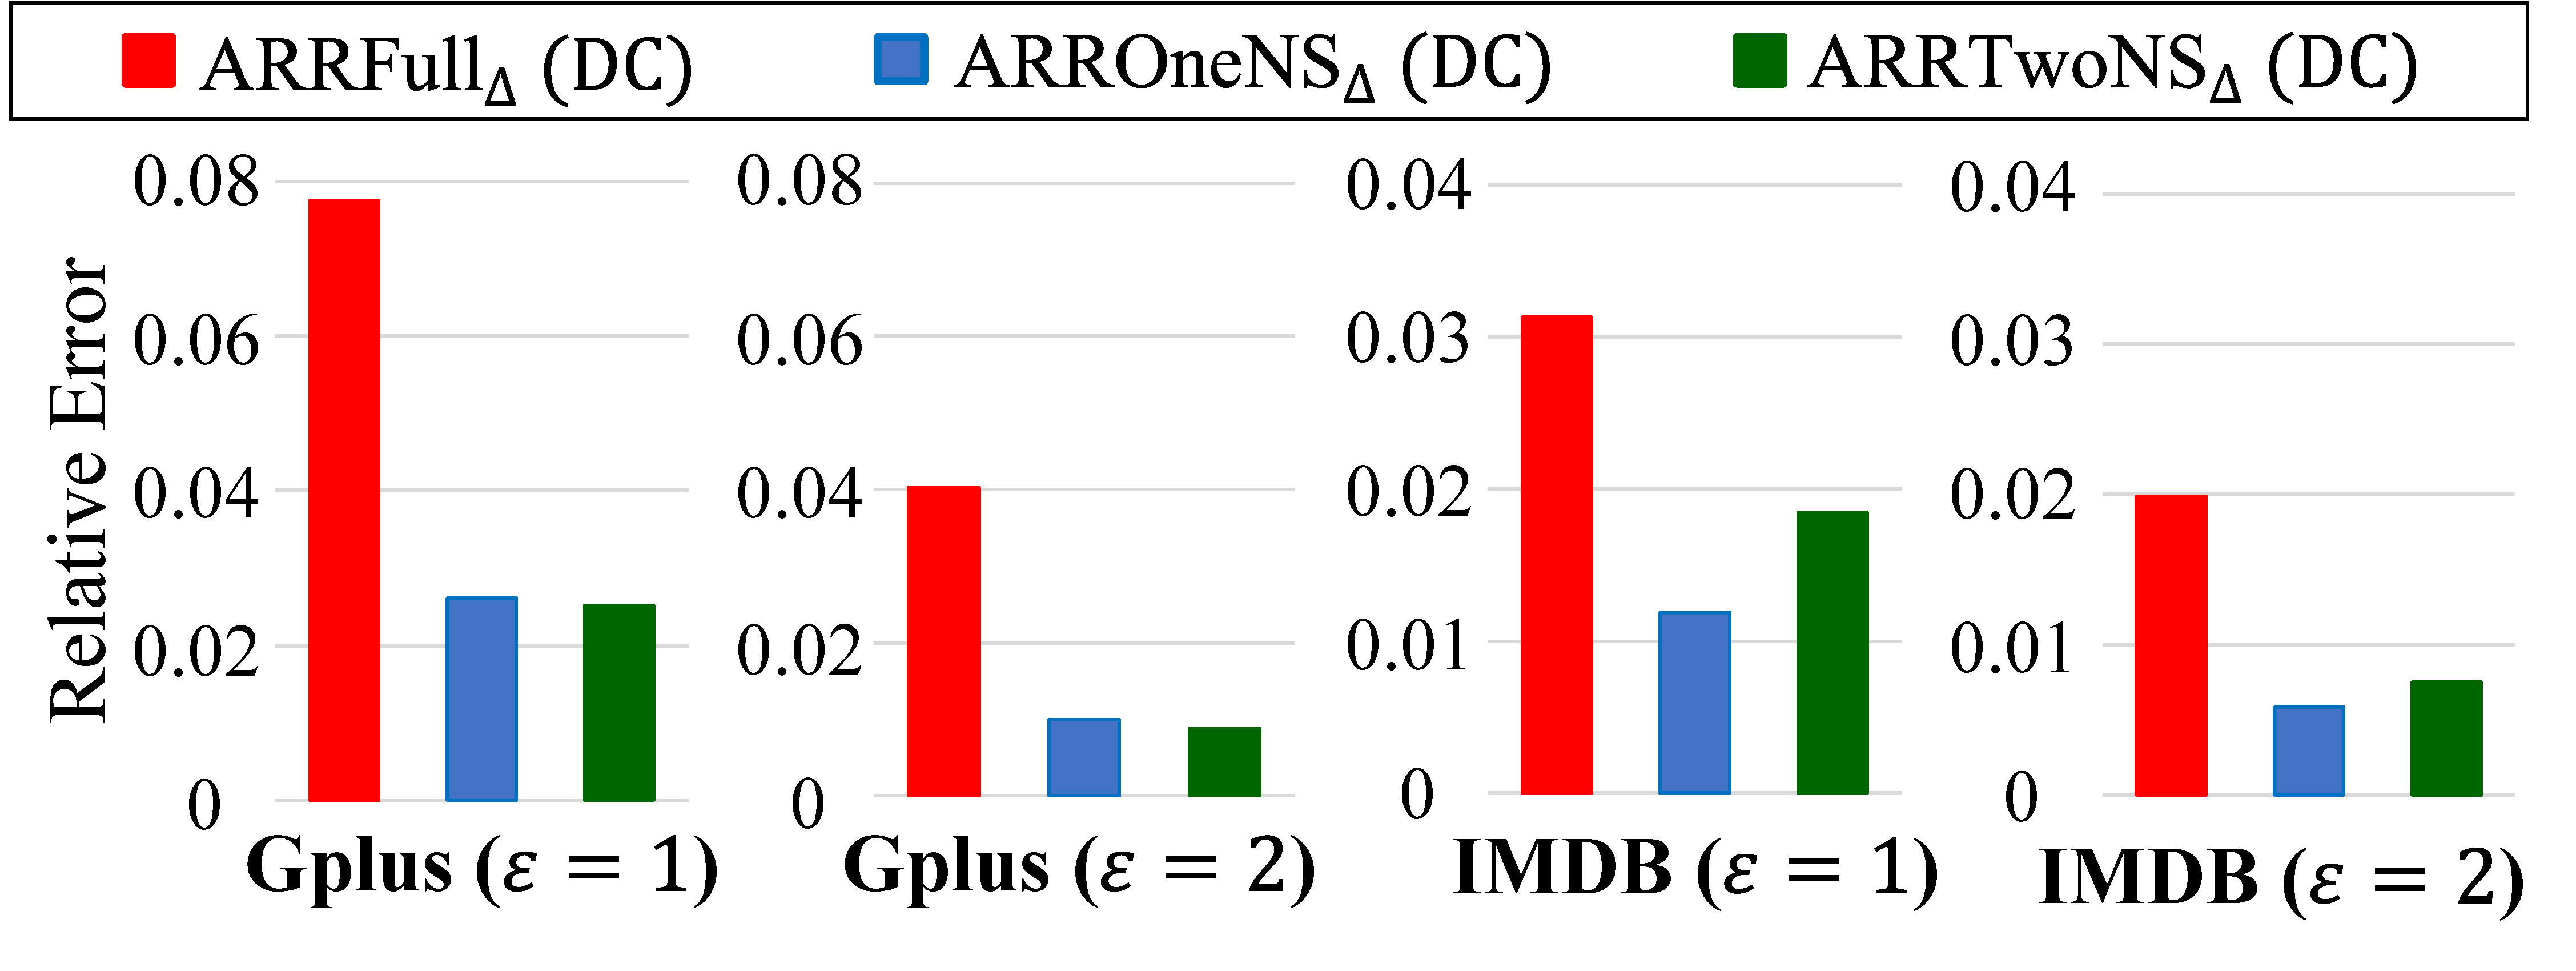
\includegraphics[width=0.96\linewidth]{fig/res2_w_Lap_abst2.pdf}
  \vspace{-6mm}
  \caption{Relative error of our three algorithms with double clipping (``DC'') when $\epsilon=1$ or $2$ and %$\mu_F=10^{-3}$ 
  $\mu^*=10^{-3}$ 
  ($n=107614$ in \GPlus{}, $n=896308$ in \IMDB{}).} 
  \label{chap2-fig:res2_w_Lap_abst}
%\end{figure}
 \vspace{1mm}
%\begin{figure}[t]
  \centering
  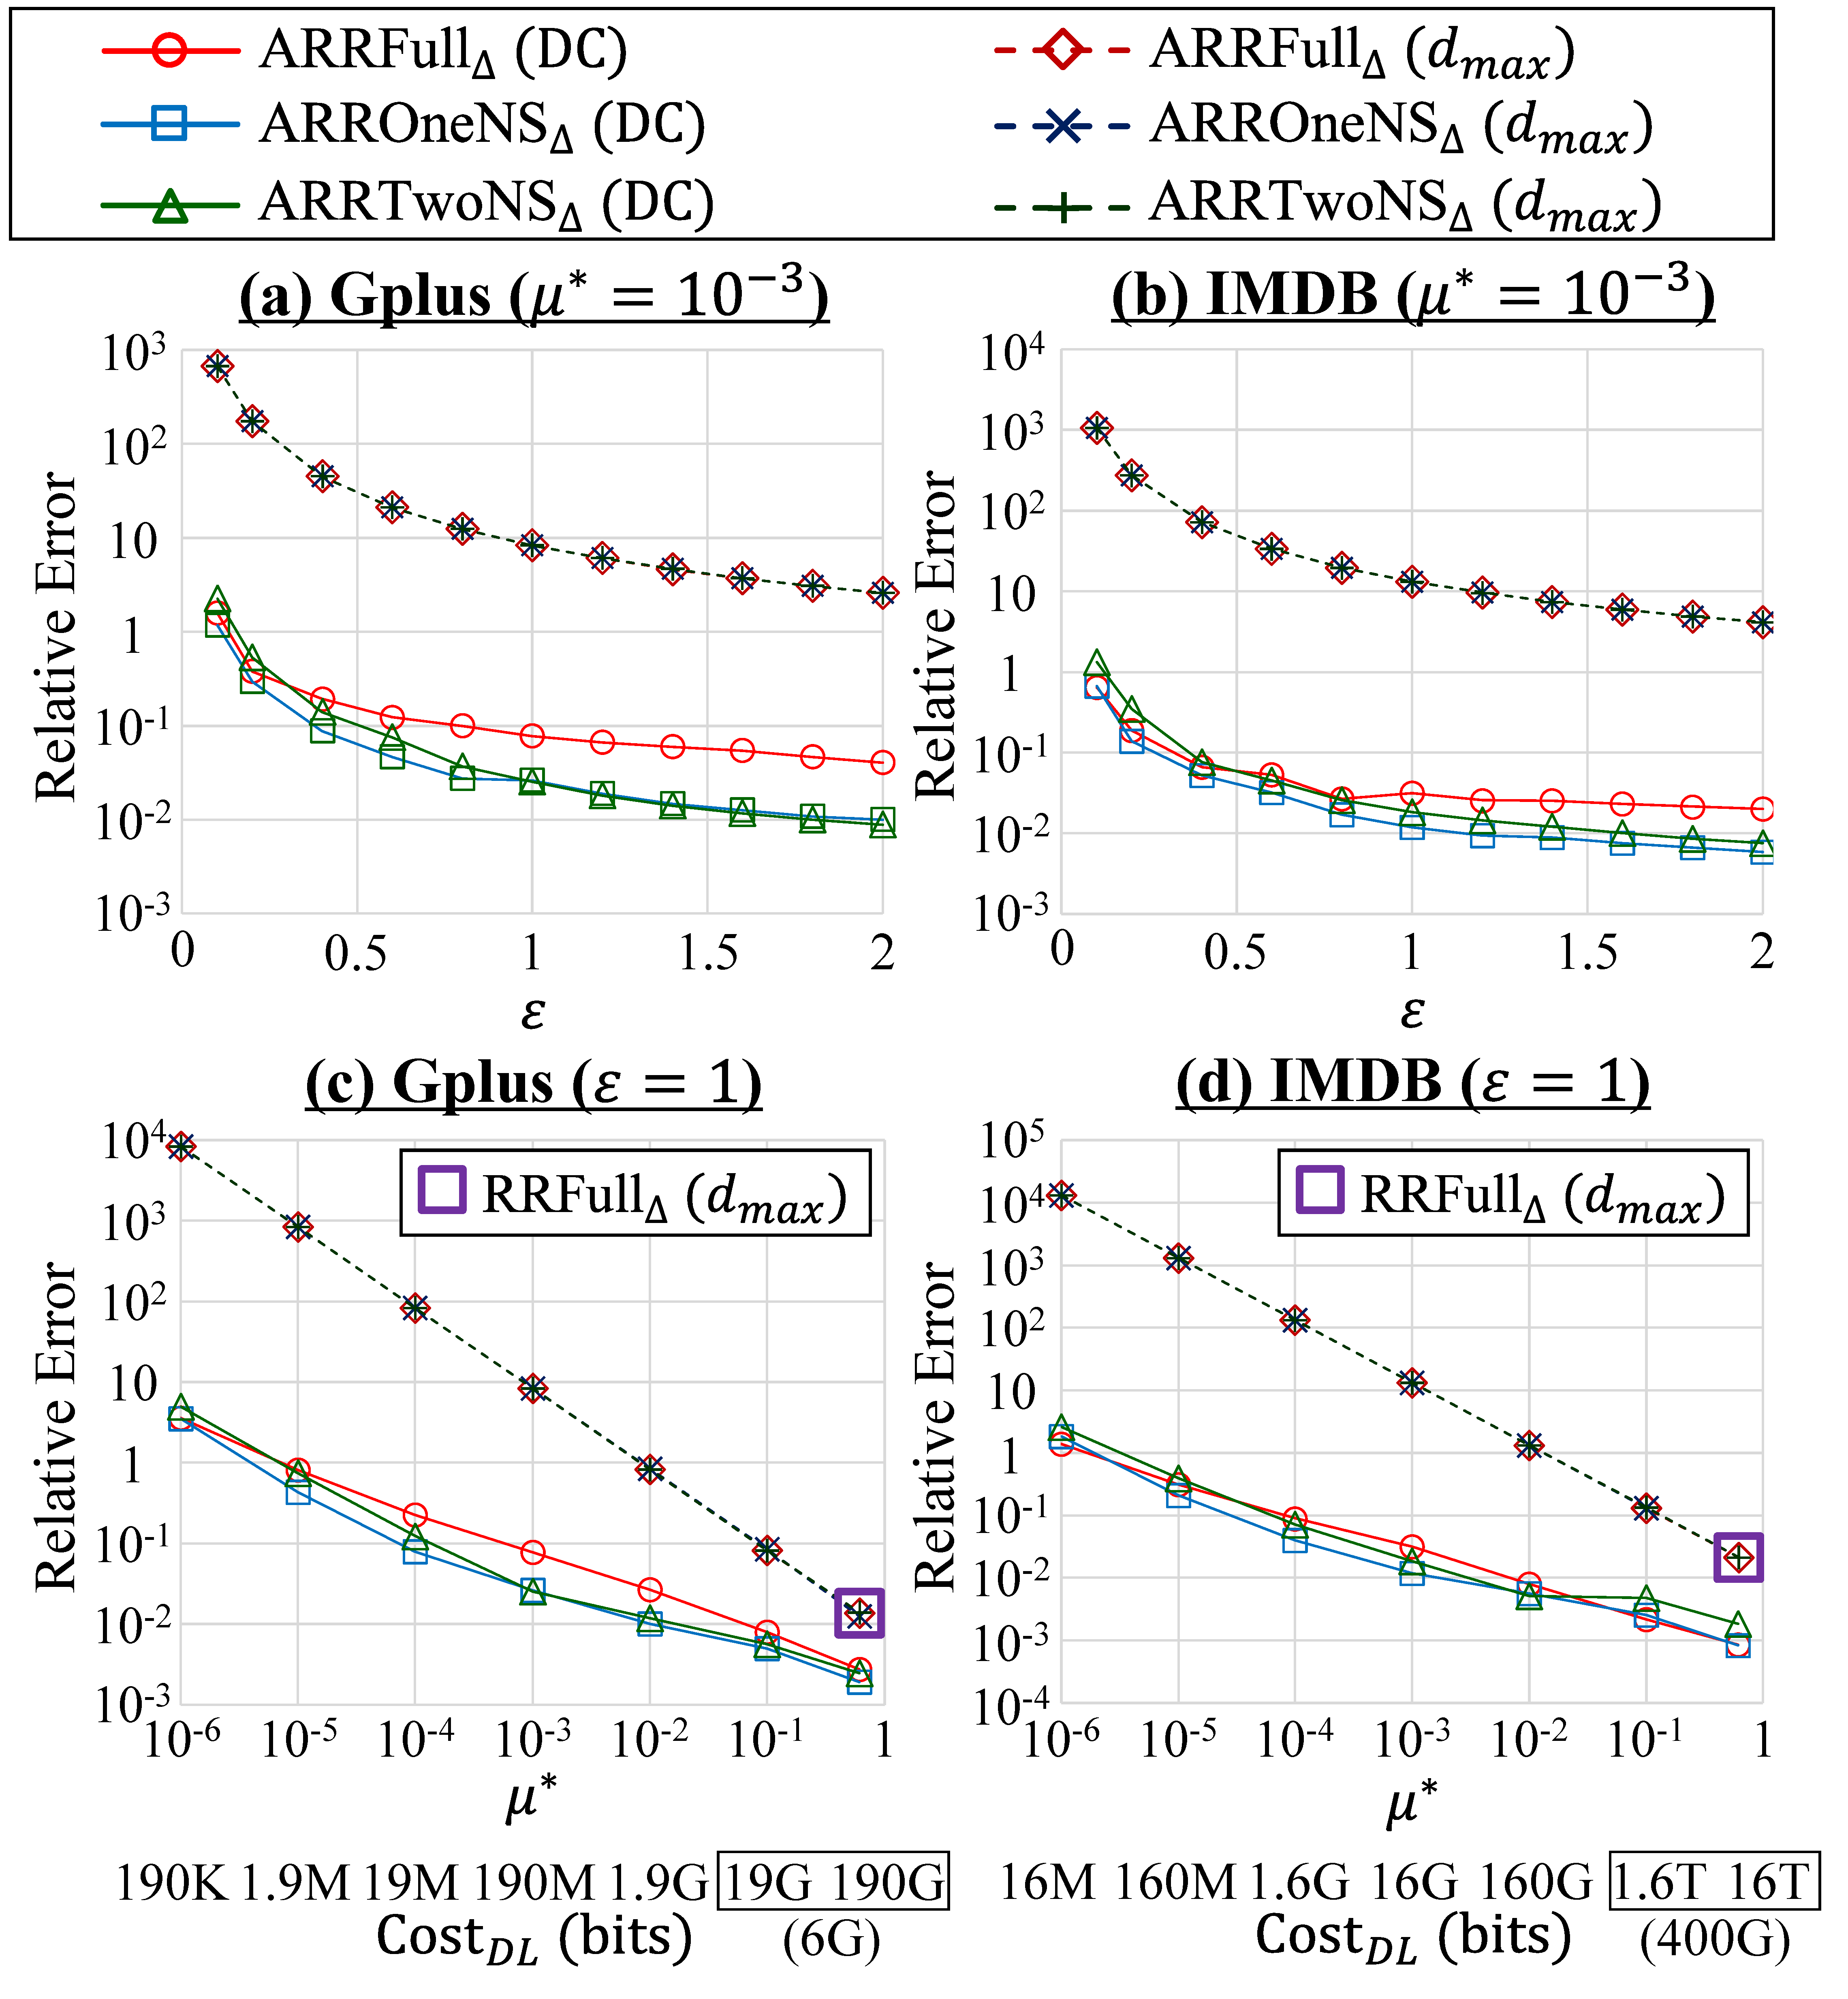
\includegraphics[width=0.99\linewidth]{fig/res2_w_Lap.pdf}
  \vspace{-5mm}
  \caption{Relative error of our three algorithms with (``DC'') or without (``$d_{max}$'') double clipping ($n=107614$ in \GPlus{}, $n=896308$ in \IMDB{}). \AlgSec{} is the 
  %two-rounds 
  algorithm in~\cite{Imola_USENIX21}. 
  $\CostDL$ is 
  %calculated by 
  an upper-bound in 
  (\ref{chap2-eq:CostDL_F}). 
  %Note that 
  When $\mu^* \geq 0.1$, 
  %(marked with squares), 
  $\CostDL$ can be $6$ Gbits and $400$ Gbits in \GPlus{} and \IMDB{}, respectively, by downloading only 0/1 for each pair of users $(v_j,v_k)$.} 
  \label{chap2-fig:res2_w_Lap}
\end{figure}

% \begin{table}[t]
% \caption{Basic notations.} 
% \centering
% \hbox to\hsize{\hfil
% \begin{tabular}{l|l|l}
% \hline
% Algorithm		&	\GPlus{} ($\epsilon=1$) &  \IMDB{}  ($\epsilon=1$)\\
% \hline
% \AlgOne{}   &   $0.078$   &   $0.031$\\
% \hline
% \end{tabular}
% \hfil}
% \label{chap2-tab:res2_w_Lap_abst}
% \end{table}

Figures~\ref{chap2-fig:res2_w_Lap_abst} and \ref{chap2-fig:res2_w_Lap} show the results. 
Figure~\ref{chap2-fig:res2_w_Lap_abst} highlights the relative error of our three algorithms with double clipping when $\epsilon=1$ or $2$ and $\mu^*=10^{-3}$. 
% Figure \ref{chap2-fig:res2_w_Lap} shows the results. 
``DC'' (resp.~``$d_{max}$'') represents algorithms with (resp.~without) double clipping. 
\AlgSec{} (marked with purple square) in Figure~\ref{chap2-fig:res2_w_Lap} (c) and (d) represents the two-rounds algorithm in~\cite{Imola_USENIX21}. 
Note that this is a special case of our \AlgOne{} without sampling ($\mu =\frac{e^{\epsilon_1}}{e^{\epsilon_1}+1} = 0.62$). 
% as described in Section~\ref{chap2-sub:algorithms_overview}. 
Figure~\ref{chap2-fig:res2_w_Lap} (c) and (d) also show the download cost $\CostDL$ calculated by 
(\ref{chap2-eq:CostDL_F}). 
Note that 
when $\mu^* \geq 0.1$ (marked with squares), 
$\CostDL$ can be $6$Gbits and $400$Gbits in \GPlus{} and \IMDB{}, respectively, by downloading only 0/1 for each pair of users $(v_j,v_k)$; $\CostDL = \frac{(n-1)(n-2)}{2}$ in this case. 
% $\CostDL$ is $400$Gbits and $6$Gbits in \GPlus{} and \IMDB{}, respectively, when user $v_i$ downloads only 0/1 for each 
% pair of users $(v_j,v_k)$ ($\CostDL = \frac{(n-1)(n-2)}{2}$ in this case). 

Figures~\ref{chap2-fig:res2_w_Lap_abst} and \ref{chap2-fig:res2_w_Lap} show that our \AlgTwo{} (DC) 
% with double clipping 
provides the best (or almost the best) performance in all cases. 
This is because \AlgTwo{} (DC) introduces the $4$-cycle trick 
% (shown in Figure~\ref{chap2-fig:four-cycle}) 
and effectively reduces the global sensitivity of the Laplacian noise by double clipping. 
% \AlgThree{} (DC) is outperformed by \AlgTwo{} (DC), 
% \AlgTwo{} (DC) outperforms \AlgThree{} (DC), 
% especially when $\epsilon$ or $\mu_F$ ($=\mu_O^2 = \mu_T^3$) is small 
% (e.g., $\epsilon=0.1$ to $0.8$, $\mu_F=10^{-6}$ to $10^{-4}$). 
% There are two reasons for this: 
% (1) \AlgThree{} cannot effectively reduce the global sensitivity by double clipping,
% (2) the Laplacian noise increases with decrease in $\epsilon$ or $\mu_F$, 
% This is because \AlgThree{} cannot effectively reduce the global sensitivity by double clipping and the Laplacian noise increases with decrease in $\epsilon$ or $\mu_F$ 
% and has a non-negligible effect on the estimation error for small $\epsilon$ or $\mu_F$, 
% (as shown in Table~\ref{chap2-tab:privacy_utility_cost} of Section~\ref{chap2-sub:clip_theoretical_analysis}). 
% The difference between \AlgTwo{} (DC) and \AlgOne{} (DC) is also small for very small $\epsilon$ or $\mu_F$ (e.g., $\epsilon=0.1$, $\mu_F=10^{-6}$) because the Laplacian noise is dominant in this case. 
% Later, we will also 
% provide a detailed investigation of the relation between the Laplacian noise and the relative error while changing $n$. 
% to answer our research question RQ1. 
Later, we will 
% also 
% provide a detailed investigation of 
investigate 
the effectiveness of the $4$-cycle trick in detail 
by not adding the Laplacian noise. 
% and 
We will also investigate 
%the relation between the Laplacian noise and the relative error 
the impact of the Laplacian noise 
while changing $n$. 

Figure~\ref{chap2-fig:res2_w_Lap} also shows that 
the relative error is almost the same between our three algorithms without double clipping (``$d_{max}$'') and that it is too large. 
% the relative error of our three algorithms without double clipping is too large and that it is almost the same between the three. 
This is because $\Lap(\frac{d_{max}}{\epsilon_2}$) is too large and dominant. 
The relative error is significantly reduced by introducing our double clipping in all cases. 
% For example, our \AlgTwo{} (DC) without sampling ($\mu_F =\frac{e^{\epsilon_1}}{e^{\epsilon_1}+1}$)
For example, when $\mu^* = 10^{-3}$, our double clipping reduces the relative error of \AlgTwo{} by two or three orders of magnitude. 
% \AlgTwo{} (DC) also reduces the expected download size by $\mu_F = \mu_O^2 = 10^{-3}$ while keeping roughly the same relative error as the algorithm in~\cite{Imola_USENIX21}, thanks to double clipping. 
The improvement is larger for smaller $\mu^*$. 

In \conference{the full version \cite{Imola_arXiv22}}\arxiv{Appendix~\ref{chap2-sec:EC_DC}}, we also evaluate the effect of edge clipping and noisy triangle clipping independently and show that each component significantly reduces the relative error. 

\smallskip
\noindent{\textbf{Communication Cost.}}~~From Figure~\ref{chap2-fig:res2_w_Lap} (c) and (d), we can explain how much our algorithms can reduce the download cost while keeping high utility, e.g., relative error $\ll 1$. 

For example, when we use the algorithm in \cite{Imola_USENIX21}, the download cost is 
$\CostDL = 400$ Gbits in \IMDB{}. 
% $\CostDL = 400$ Gbits and $6$ Gbits in \GPlus{} and \IMDB{}, respectively. 
Thus, when the download speed is $20$ Mbps 
% (which is a 
(recommended speed in YouTube \cite{YouTube_speed}), every user $v_i$ needs 6 hours to download the message $M_i$, which is far from practical. 
In contrast, our \AlgTwo{} (DC) can reduce it to 
% $100$ 
$160$ 
Mbits (8 seconds when $20$ Mbps download rate) or less 
while keeping relative error $= 0.21$, 
% (relative error $= 0.21$), 
% or $1$ Gbits (relative error $= 0.040$). 
% Consequently, every user needs only 
% 5 
% 8 
% or 50 
% seconds or less, 
which is practical and a dramatic improvement over \cite{Imola_USENIX21}. 
% Therefore, private triangle counting is now practical.

We also note that since $d_{max} \ll n$ in \IMDB{}, 
% the ARR outputs ``1'' with probability $\mu e^{-\epsilon_1}$ in most cases
% the download cost 
$\CostDL$ of our \AlgTwo{} (DC) 
can also be roughly approximated by $60$ Mbits (3 seconds) by replacing $\mu$ with $\mu e^{-\epsilon_1}$ in 
(\ref{chap2-eq:CostDL_F}). 
%(\ref{chap2-eq:CostDL_O}). 

% We also note that the upload cost is much smaller; e.g., by (\ref{chap2-eq:CostUL_proposal}), $\CostUL{} = 11$ Mbits in \IMDB{} even when $\mu=1$. 
% Thus, it is not an issue.

\smallskip
% \noindent{\textbf{Three Algorithms w/o Lap.}}~~
\noindent{\textbf{4-Cycle Trick.}}~~We 
% first evaluated 
also investigated 
% how well our two algorithms \AlgTwo{} and \AlgThree{} address the $4$-cycle issue of \AlgOne{} 
the effectiveness of our $4$-cycle trick in \AlgTwo{} and \AlgThree{} 
% (shown in Figure~\ref{chap2-fig:four-cycle}) 
in detail. 
% explained in Section~\ref{chap2-sub:algorithms_overview}. 
% the relation between the $4$-cycle issue 
To this end, we evaluated our three algorithms when we did \textit{not} add the Laplacian noise at the second round. 
% (i.e., $\epsilon_2 = \infty$). 
Note that they do not provide edge LDP, as $\epsilon_2 = \infty$. 
The purpose here is to purely investigate the effectiveness of the $4$-cycle trick 
% issue 
related to our first research question RQ1. 
% We will report experimental results of the three algorithms with the Laplacian noise later. 

\begin{figure}[t]
  \centering
  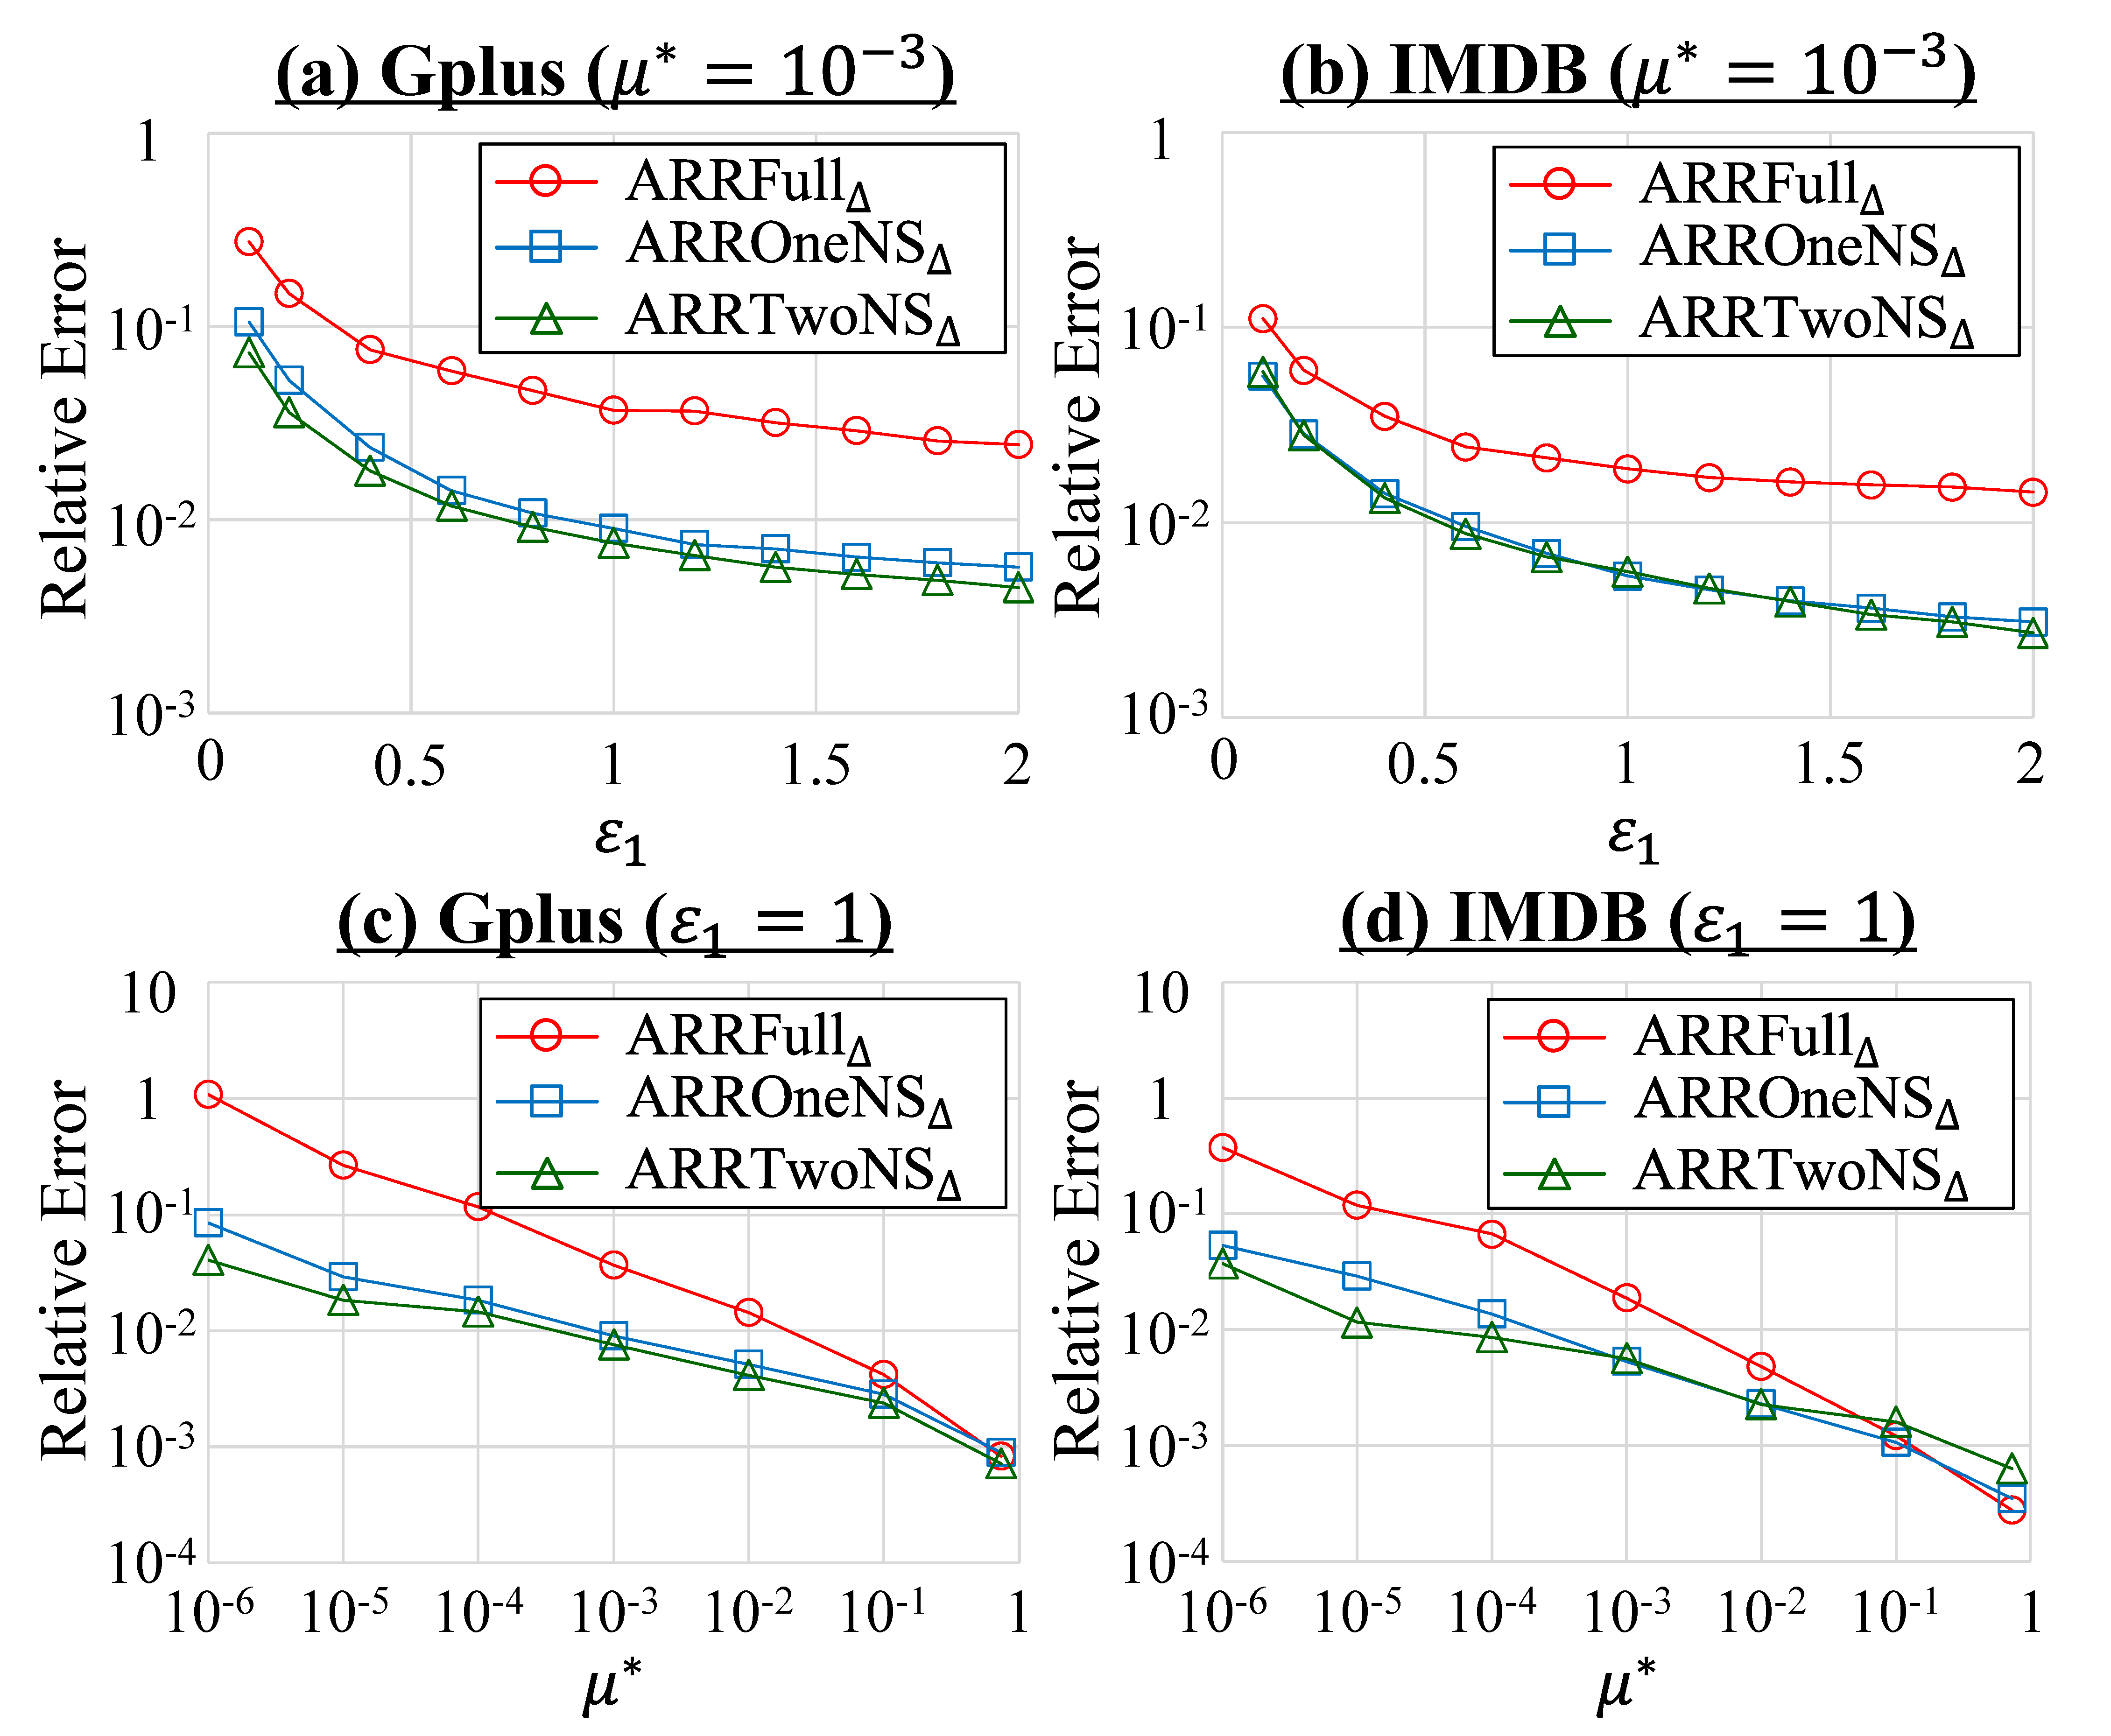
\includegraphics[width=0.99\linewidth]{fig/res1_wo_Lap.pdf}
  \vspace{-5mm}
  \caption{Relative error of our three algorithms without the Laplacian noise 
  % at the second round 
  ($n=107614$ in \GPlus{}, $n=896308$ in \IMDB{}).} 
  \label{chap2-fig:res1_wo_Lap}
\end{figure}

% We first evaluated our three triangle counting algorithms with double clipping. 
Figure~\ref{chap2-fig:res1_wo_Lap} shows the results, where 
% $\mu_F$ (resp.~$\epsilon_1$) is changed from $10^{-6}$ to $1$ (resp.~$0.1$ to $2$). 
% $\epsilon_1$ (resp.~$\mu_F$) is changed from $0.1$ to $2$ (resp.~$10^{-6}$ to $\frac{e^{\mu_F}}{e^{\mu_F} + 1}$). 
$\epsilon_1$ and 
% $\mu_F$ ($= \mu_O^2 = \mu_T^3$) 
$\mu^*$ 
are changed to various values. 
Figure~\ref{chap2-fig:res1_wo_Lap} shows that \AlgTwo{} and \AlgThree{} significantly outperform \AlgOne{} when 
% $\mu_F$ 
$\mu^*$ 
is small. 
This is because in both \AlgTwo{} and \AlgThree{}, 
% the first term in the expected $l_2$ loss 
the factors of 
% $S_3$ (\#3-stars) and $P_3$ (\#3-paths) 
$C_4$ (\#4-cycles) and $S_3$ (\#3-stars) 
in the expected $l_2$ loss 
diminish 
for small $\mu$, 
% as 
% $\mu_F$ ($= \mu_O^2 = \mu_T^3$) 
% the parameter $\mu$ in the ARR 
% goes to $0$, 
as explained in Section~\ref{chap2-sub:algorithms_theoretical_analysis}. 
In other words, \AlgTwo{} and \AlgThree{} effectively address the $4$-cycle issue. 
Figure~\ref{chap2-fig:res1_wo_Lap} also shows that \AlgThree{} slightly outperforms \AlgTwo{} when $\mu^*$ is small. 
% (e.g., $10^{-6}$ to $10^{-4}$). 
This is because 
% the first term in the expected $l_2$ loss diminishes 
% the factors of $S_3$ and $P_3$ 
the factors of $C_4$ and $S_3$ 
diminish 
more rapidly; i.e., \AlgThree{} addresses the $4$-cycle issue more aggressively. 

However, when we add the Laplacian noise, \AlgThree{} (DC) is outperformed by \AlgTwo{} (DC), as shown in Figure~\ref{chap2-fig:res2_w_Lap}. 
% \AlgTwo{} (DC) outperforms \AlgThree{} (DC), 
% especially when $\epsilon$ or $\mu_F$ ($=\mu_O^2 = \mu_T^3$) is small 
% (e.g., $\epsilon=0.1$ to $0.8$, $\mu_F=10^{-6}$ to $10^{-4}$). 
This is because \AlgThree{} cannot effectively reduce the global sensitivity by double clipping. 
In Figure~\ref{chap2-fig:res2_w_Lap}, the difference between \AlgTwo{} (DC) and \AlgOne{} (DC) is also small for very small $\epsilon$ or $\mu^*$ (e.g., $\epsilon=0.1$, $\mu^*=10^{-6}$) because the Laplacian noise is dominant in this case. 
% (as shown in Table~\ref{chap2-tab:privacy_utility_cost} of Section~\ref{chap2-sub:clip_theoretical_analysis}). 

\smallskip
\noindent{\textbf{Changing $\bm{n}$.}}~~We 
finally 
% also 
evaluated our three algorithms with double clipping while changing the number $n$ of users. 
In both \GPlus{} and \IMDB{}, we randomly selected $n$ users from all users and extracted a graph with $n$ users. 
Then we evaluated the relative error while changing $n$ to various values.

\begin{figure}[t]
  \centering
  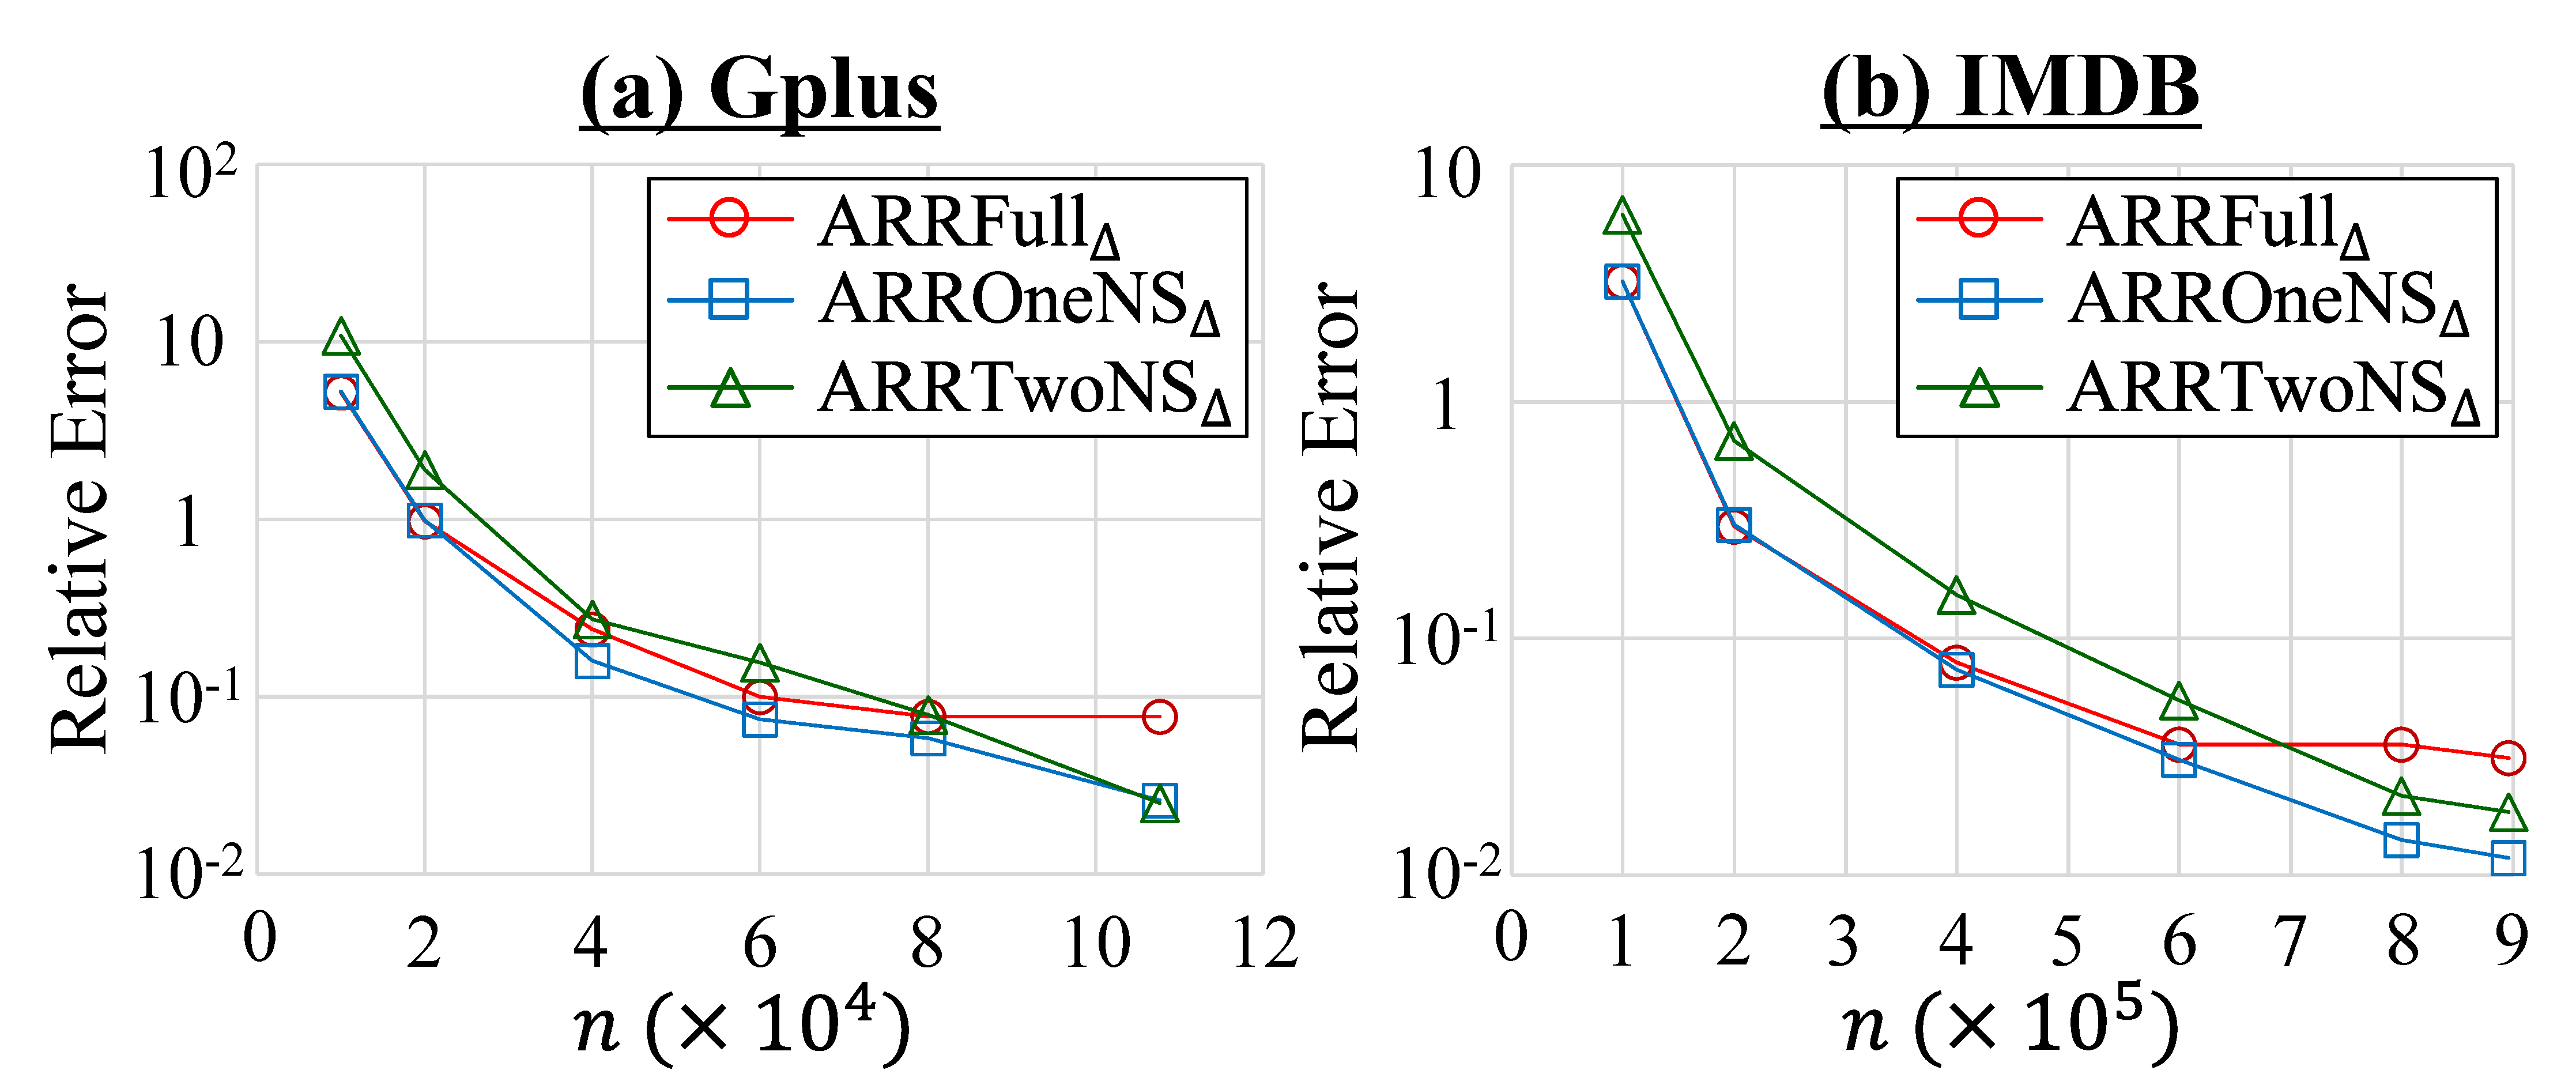
\includegraphics[width=0.99\linewidth]{fig/res3_n.pdf}
  \vspace{-4mm}
  \caption{Relative error of our three algorithms with double clipping for various values of $n$ 
  ($\epsilon=1$, $\mu^*=10^{-3}$).} 
  \label{chap2-fig:res3_n}
\end{figure}

Figure~\ref{chap2-fig:res3_n} shows the results, where $\epsilon=1$ ($\epsilon_0=0.1$, $\epsilon_1 = \epsilon_2 = 0.45$) and $\mu^* = 10^{-3}$. 
In all 
% the 
three algorithms, the relative error decreases with increase in $n$.
This is because the expected $l_2$ loss can be expressed as 
% $O(n)$ (when we regard $\epsilon$ and $\mu_F$ as constants and ignore $d_{max}$) 
$O(n d_{max}^3)$ or $O(n d_{max}^2)$ 
% (when we regard $\epsilon$ as constants) 
in these algorithms as shown in Section~\ref{chap2-sub:clip_theoretical_analysis} and the square of the true triangle count can be expressed as $\Omega(n^2)$.
In other words, when $d_{max} \ll n$, the relative error becomes smaller for larger $n$. 
% In other words, this is consistent with our theoretical results. 
Figure~\ref{chap2-fig:res3_n} also shows that for small $n$, \AlgThree{} provides the worst performance and 
\AlgTwo{} performs almost the same as \AlgOne{}. 
% the difference between \AlgTwo{} and \AlgOne{} is very small. 
For large $n$, 
% \AlgThree{} outperforms \AlgOne{} and 
\AlgOne{} performs the worst and 
\AlgTwo{} performs the best. 


To investigate the reason for this, we decomposed the estimation error into two components -- 
the first error caused by empirical estimation and the second error caused by the Laplacian noise. 
Specifically, for each algorithm, 
we evaluated the first error by calculating the relative error when we did not add the Laplacian noise ($\epsilon_1 = 0.45$). 
Then we evaluated the second error by subtracting the first error from the relative error when we used double clipping ($\epsilon_0=0.1$, $\epsilon_1 = \epsilon_2 = 0.45$). 

Figure~\ref{chap2-fig:res3_emp_Lap} shows the results for some values of $n$, where ``emp'' represents the first error by empirical estimation and ``Lap'' represents the second error by the Laplacian noise. 
We observe that the second error 
rapidly decreases with increase in $n$. 
% The difference between \AlgOne{} and \AlgTwo{} 
% This is because the expected $l_2$ loss of the Laplacian noise is $O(\sum_{i=1}^n \kappa_i^2)$, 
% which is much smaller than $O(n d_{max}^2)$, 
% as shown in Section~\ref{chap2-sub:clip_theoretical_analysis}. 
In addition, 
% Figure~\ref{chap2-fig:res3_emp_Lap} also shows that 
the first error of \AlgOne{} is much larger than those of \AlgTwo{} and \AlgThree{} when $n$ is large. 

We also examined 
% the maximum degree $d_{max}$ and 
the number $C_4$ of $4$-cycles as a function of $n$. Figure~\ref{chap2-fig:res4_4cycles} shows the results. 
We observe that $C_4$ (which is $O(n d_{max}^3)$) is quartic in $n$; e.g., $C_4$ is increased by $2^4 \approx 10$ and $6^4 \approx 10^3$ when $n$ is multiplied by $2$ and $6$, respectively. 
This is because we randomly selected $n$ users from all users and $d_{max}$ is almost proportional to $n$ (though $d_{max} \ll n$). 
% We observe that $d_{max}$ is proportional to $n$ (though $d_{max} \ll n$). 
% This is because we randomly selected $n$ users from all users. 
% Consequently, $C_4$ which can be expressed as $O(n d_{max}^3)$ is quartic in $n$; e.g., $C_4$ is increased by $2^4 \approx 10$ and $6^4 \approx 10^3$ when $n$ is multiplied by $2$ and $6$, respectively. 

\begin{figure}[t]
  \centering
  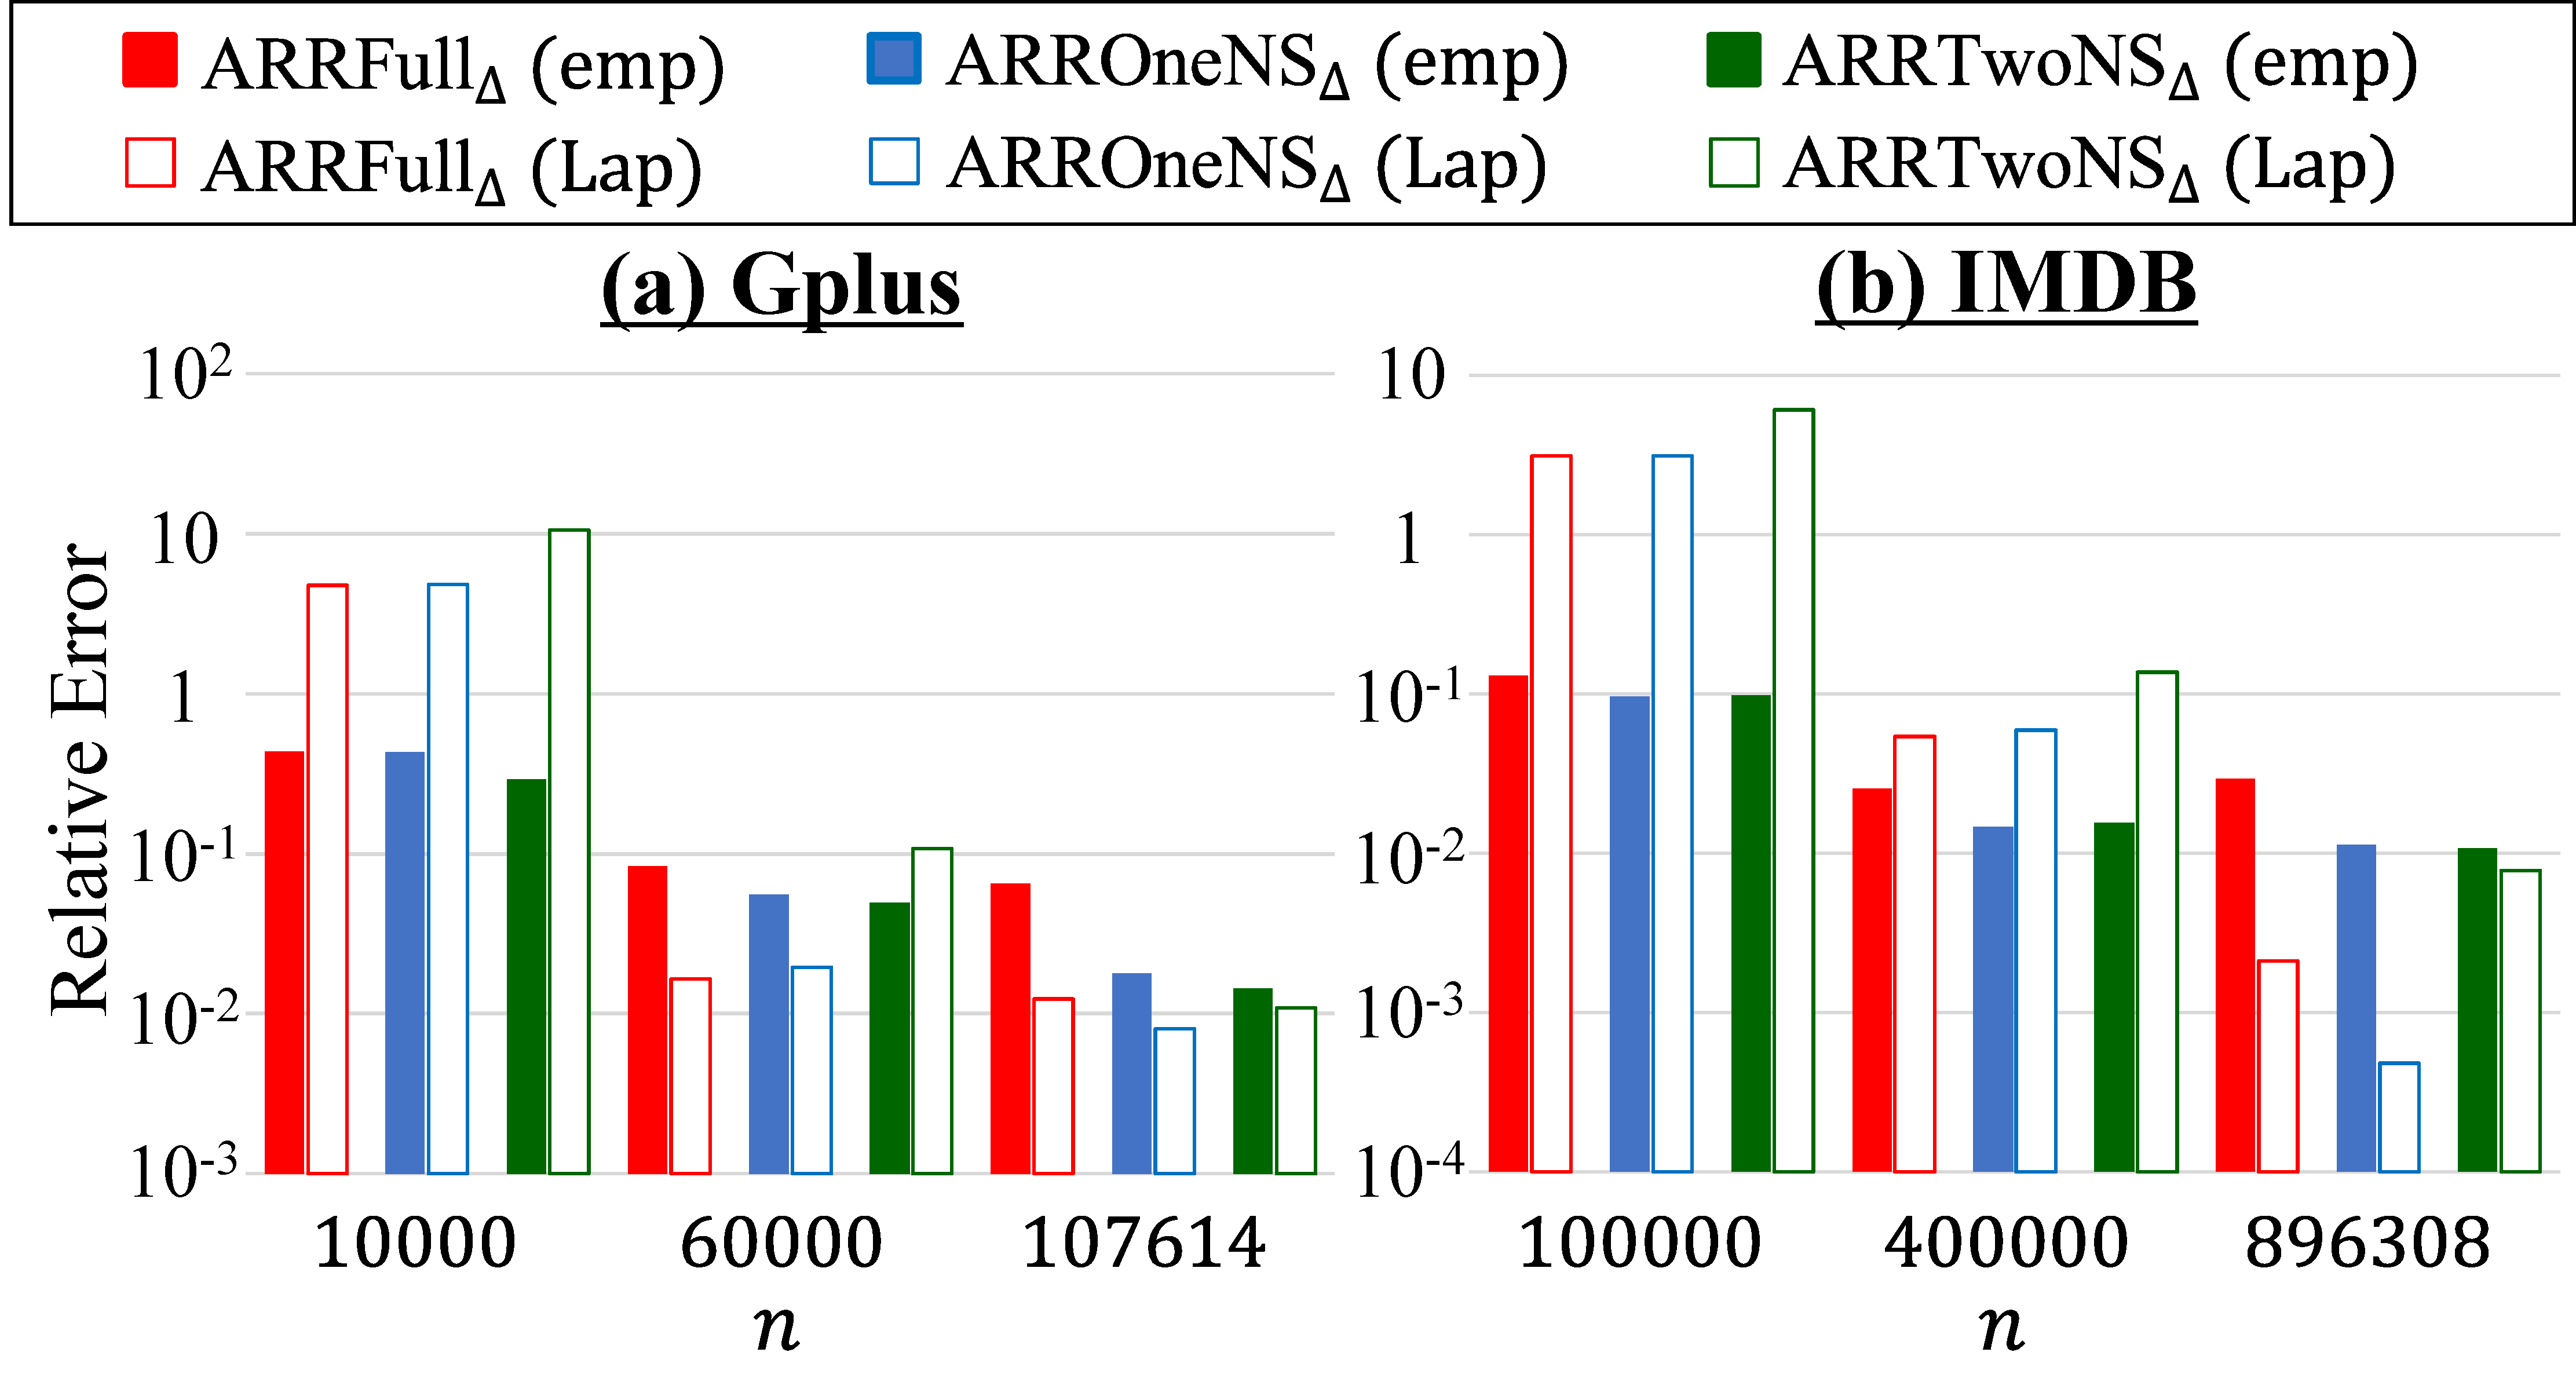
\includegraphics[width=0.99\linewidth]{fig/res3_emp_Lap.pdf}
  \vspace{-5mm}
  \caption{Relative error of empirical estimation and the Laplacian noise in our three algorithms with double clipping ($\epsilon=1$, $\mu^*=10^{-3}$).} 
  \label{chap2-fig:res3_emp_Lap}
% \end{figure}
 \vspace{1mm}
% \begin{figure}[t]
  \centering
  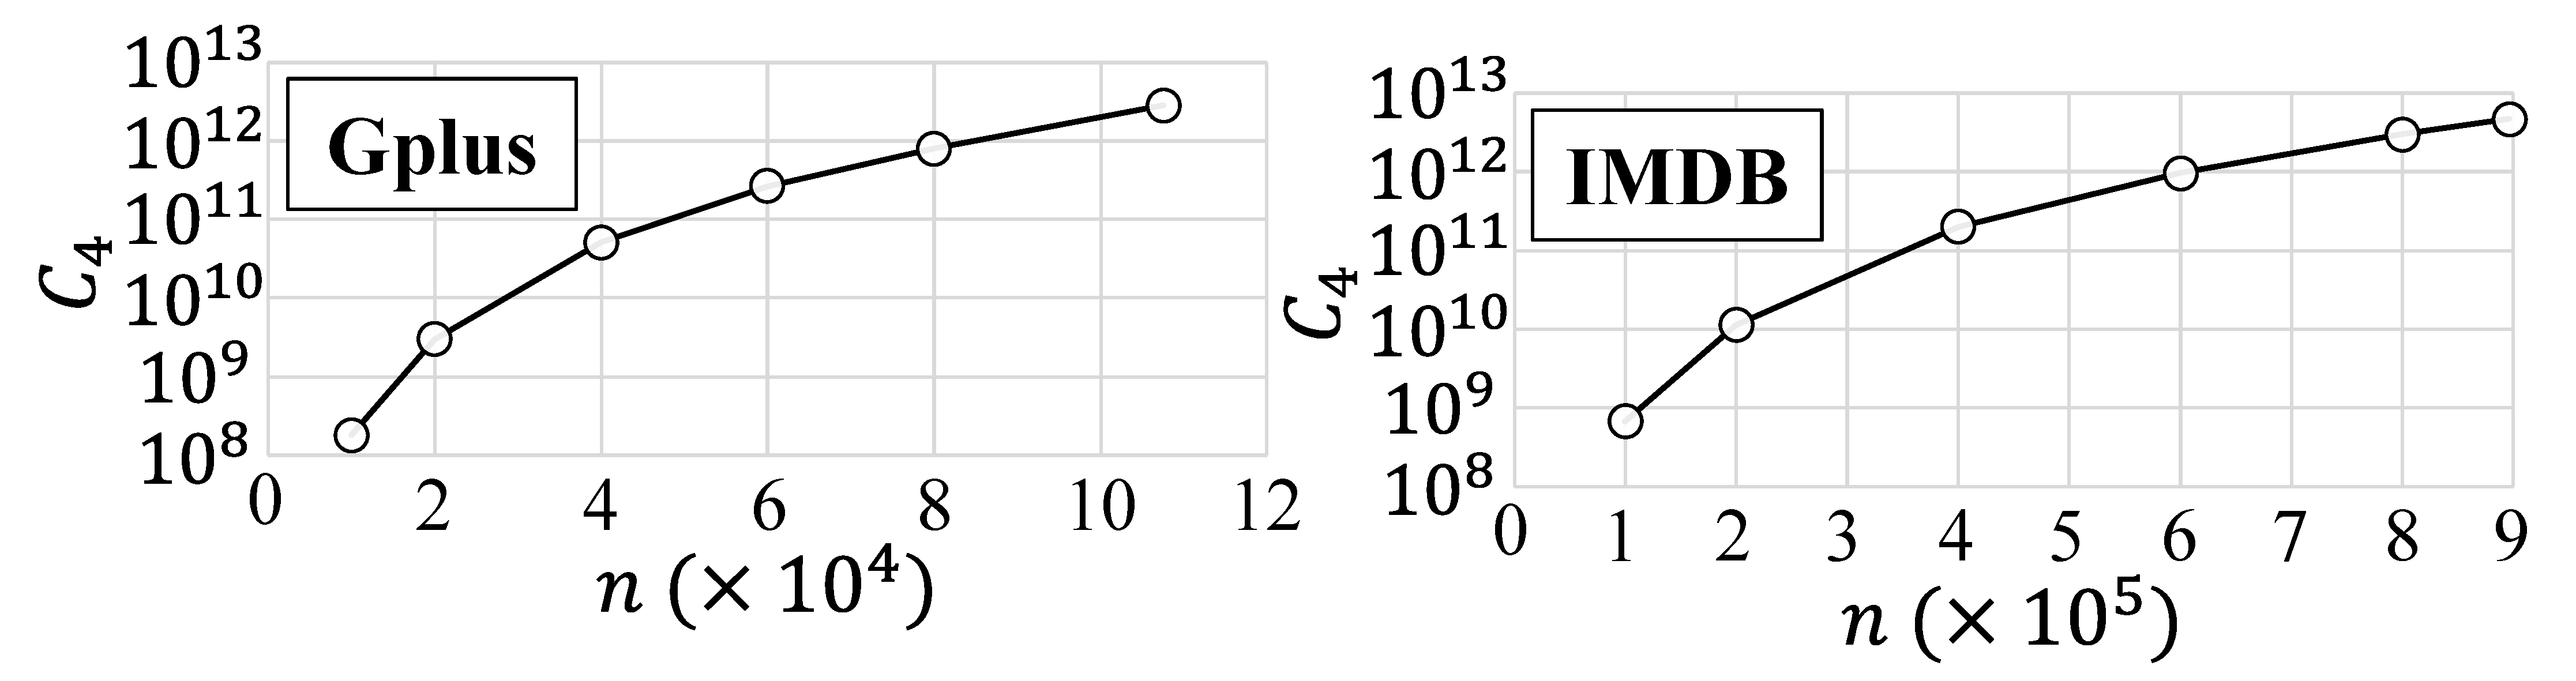
\includegraphics[width=0.99\linewidth]{fig/res4_4cycles.pdf}
  \vspace{-5mm}
%   \caption{Maximum degree $d_{max}$ and \#$4$-cycles $C_4$.} 
  \caption{\#$4$-cycles $C_4$.} 
  \label{chap2-fig:res4_4cycles}
\end{figure}

Based on Figures~\ref{chap2-fig:res3_emp_Lap} and \ref{chap2-fig:res4_4cycles}, we can explain 
% the results in 
Figure~\ref{chap2-fig:res3_n} as follows. 
As shown in Section~\ref{chap2-sub:clip_theoretical_analysis}, the $l_2$ loss of empirical estimation can be expressed as 
% $O(\frac{n d_{max}^3}{\mu_F})$, $O(\frac{n d_{max}^2}{\mu_O^2})$, and $O(\frac{n d_{max}^2}{\mu_T^3})$ 
$O(n d_{max}^3)$, $O(n d_{max}^2)$, and $O(n d_{max}^2)$ 
in \AlgOne{}, \AlgTwo{}, and \AlgThree{}, respectively. 
% when 
% we regard $\epsilon$ as a constant.
% $\mu_F$ ($= \mu_O^2 = \mu_T^3$) 
% $\mu^*$ is small.  
The large $l_2$ loss of \AlgOne{} is caused by a large value of $C_4$. 
% as shown in Figure~\ref{chap2-fig:res4_4cycles}. 
% the $4$-cycle issue. 
% When 
% $\mu_F$ is small, 
% $n$ is small, 
% the Laplacian noise has a non-negligible impact on the estimation error. 
% as explained in Section~\ref{chap2-sub:clip_theoretical_analysis}. 
% However, 
The expected $l_2$ loss of the Laplacian noise is 
$O(\sum_{i=1}^n \kappa_i^2)$, 
% $O(\sum_{i=1}^n \lambda_i^2 \td_i^2)$, 
which is much smaller than $O(n d_{max}^2)$. 
Thus, 
% when $n$ is large, 
as $n$ increases, 
% when $d_{max}$ is proportional to $n$, 
% as in Figure~\ref{chap2-fig:res4_4cycles}, 
the Laplacian noise becomes relatively very small, 
% rapidly decreases with increase in $n$ 
as shown in Figure~\ref{chap2-fig:res3_emp_Lap}. 
Consequently, \AlgTwo{} provides the best performance for large $n$ because it addresses the $4$-cycle issue 
and effectively reduces the global sensitivity. 
This explains the results in Figure~\ref{chap2-fig:res3_n}. 
It is also interesting that when $n \approx 10^5$, \AlgOne{} performs the worst in \GPlus{} and almost the same as \AlgTwo{} in \IMDB{} (see Figure~\ref{chap2-fig:res3_n}). 
This is because \GPlus{} is more dense than \IMDB{} 
% (as described in Section~\ref{chap2-sub:setup}) 
and $C_4$ is much larger in \GPlus{} when $n \approx 10^5$, as in Figure~\ref{chap2-fig:res4_4cycles}.

In other words, Figures~\ref{chap2-fig:res3_n}, \ref{chap2-fig:res3_emp_Lap}, and \ref{chap2-fig:res4_4cycles} are consistent with our theoretical results in Section~\ref{chap2-sub:clip_theoretical_analysis}. 
From these results, we conclude that \AlgTwo{} is effective especially for 
a large graph (e.g., $n \approx 10^6$) or dense graph (e.g., \GPlus{}) where the number $C_4$ of $4$-cycles is large. 
% a graph that has a large number of $4$-cycles. 
% In Appendix~\ref{chap2-sec:BAmodel}, we also show similar results using the Barab\'{a}si-Albert graph model.



% \smallskip
% \noindent{\textbf{Communication Cost.}}~~TBD.

\smallskip
\noindent{\textbf{Summary.}}~~In summary, our answers to our three research questions RQ1-3 
% at the beginning of Section~\ref{chap2-sec:experiments} 
are as follows. 
% \begin{itemize}
%     \item Our 
% \end{itemize}
% First, 
[RQ1]: Our \AlgTwo{} achieves almost the smallest estimation error in all cases and outperforms the other two, especially for a large graph or dense graph where $C_4$ is large. 
[RQ2]: Our double clipping reduces the estimation error by two or three orders of magnitude. 
[RQ3]: Our entire algorithm (\AlgTwo{} with double clipping) dramatically reduces the communication cost, 
e.g., 
% from $400$ Gbits to $160$ Mbits or less (relative error $=0.21$) in \IMDB{}.
% When the DL speed is $20$ Mbps \cite{YouTube_speed}, the DL time is reduced from $6$ hours to $5$ seconds. 
from $6$ hours to $8$ seconds or less (relative error $=0.21$) in \IMDB{} at a $20$ Mbps download rate \cite{YouTube_speed}. 

Thus, triangle counting under edge LDP is now 
much more 
practical. 
In Appendix~\ref{chap2-sec:cluster}, we show that the clustering coefficient can also be accurately estimated using our algorithms.


\section{Conclusions}
\label{chap2-sec:conclusions}
% In this paper, we proposed
% locally private
We proposed
triangle counting algorithms under edge LDP with a small estimation error and small communication cost.
We showed that
% the estimation error can be significantly reduced by our 4-cycle trick and double clipping, and that
our entire algorithms with the 4-cycle trick and double clipping
% can 
dramatically reduce the download cost
% when compared with
of
\cite{Imola_USENIX21},
% (e.g., from $400$ Gbits to $100$ Mbits).
e.g., from 6 hours to 8 seconds or less. 
% when $20$ Mbps).
% In \cite{Imola_USENIX21},

% In this paper,
We assumed that each user $v_i$ honestly inputs her neighbor list $\bma_i$, as in most previous work on LDP.
However, recent studies \cite{Cao_USENIX21,Cheu21} show that the estimate in LDP can be skewed by data poisoning attacks.
% with a number of malicious accounts.
As future work, we would like to analyze the impact of data poisoning on our algorithms and develop defenses (e.g., detection) against it.


% %-------------------------------------------------------------------------------
\section*{Acknowledgments}
Kamalika Chaudhuri and Jacob Imola would like to thank ONR under N00014-20-1-2334 and UC Lab Fees under LFR 18-548554  for research support.
Takao Murakami was supported in part by JSPS KAKENHI JP19H04113.

%-------------------------------------------------------------------------------

%-------------------------------------------------------------------------------
\bibliographystyle{plain}
%\bibliographystyle{abbrv}
% \bibliography{main}
\bibliography{main_sshort}

\appendix

% \section{Extension of the Two-Rounds Algorithm}
% \label{sec:modified_two_rounds}
% aaa

% \section{Basic Notations}
% \label{sec:notations}

% Table~\ref{tab:notations} shows the basic notations used in this paper.

\section{Effectiveness of empirical estimation in \alg{LocalRR$_\triangle$}}
\label{sec:RR_emp}
In Section~\ref{sub:non-interactive_triangles}, we presented \alg{LocalRR$_\triangle$}, which uses the empirical estimation method after the RR. 
Here we show the effectiveness of empirical estimation by comparing \alg{LocalRR$_\triangle$} with the RR without empirical estimation \cite{Qin_CCS17,Ye_ICDE20}. 
% i.e., the randomized neighbor list in \cite{Qin_CCS17}. 
% This method was also used in \cite{Ye_ICDE20}. 
% We also note that the RR has been applied to the adjacency matrix without empirical estimation in \cite{Qin_CCS17,Ye_ICDE20} for different purposes than counting triangles. 

As the RR without empirical estimation, we applied the RR to the lower triangular part of the adjacency matrix $\bmA$; i.e., we ran lines 1 to 6 in Algorithm~\ref{alg:subgraph-rr}. 
% This is the extended version of the randomized neighbor list \cite{Qin_CCS17}, as described in Section
Then we output the number of noisy triangles $m_3$. 
We denote this algorithm by \alg{RR w/o emp}. 
% Both \alg{LocalRR$_\triangle$} and \alg{RR w/o emp} provide $\epsilon$-edge LDP and $\epsilon$-entire edge LDP. 

% \begin{table}[t]
% \caption{Basic notations in this paper.} 
% \centering
% \hbox to\hsize{\hfil
% \begin{tabular}{l|l}
% \hline
% Symbol		&	Description\\
% \hline
% $n$         &	    Number of users.\\
% $G=(V,E)$   &	    Graph with $n$ nodes (users) $V$ and edges $E$.\\
% $v_i$       &       $i$-th user in $V$.\\
% $d_{max}$   &       Maximum degree of $G$.\\
% $\td_{max}$   &       Upper-bound on $d_{max}$ (used for projection).\\
% $\calG$     &       Set of possible graphs on $n$ users.\\
% $\bmA=(a_{i,j})$	    &		Adjacency matrix.\\
% $\bma_i$	&		$i$-th row of $\bmA$ (i.e., neighbor list of $v_i$).\\
% $\calR_i$     &       Randomized algorithm on $\bma_i$.\\
% $f_\triangle(G)$   &  Number of triangles in $G$.\\
% $f_{k\star}(G)$    &  Number of $k$-stars in $G$.\\
% \hline
% \end{tabular}
% \hfil}
% \label{tab:notations}
% \end{table}

Figure~\ref{fig:res5_RR_wo_emp} shows the $l_2$ loss of \alg{LocalRR$_\triangle$} and \alg{RR w/o emp} when we changed $n$ from $1000$ to $10000$ or $\epsilon$ in edge LDP from $0.1$ to $2$. 
The experimental set-up is the same as Section~\ref{sub:setup}. 
Figure~\ref{fig:res5_RR_wo_emp} shows that \alg{LocalRR$_\triangle$} significantly outperforms \alg{RR w/o emp}, which means that the $l_2$ loss is significantly reduced by empirical estimation. 
As shown in Section~\ref{sec:experiments}, the $l_2$ loss of \alg{LocalRR$_\triangle$} is also significantly reduced by an additional round of interaction.

\begin{figure}[t]
\centering
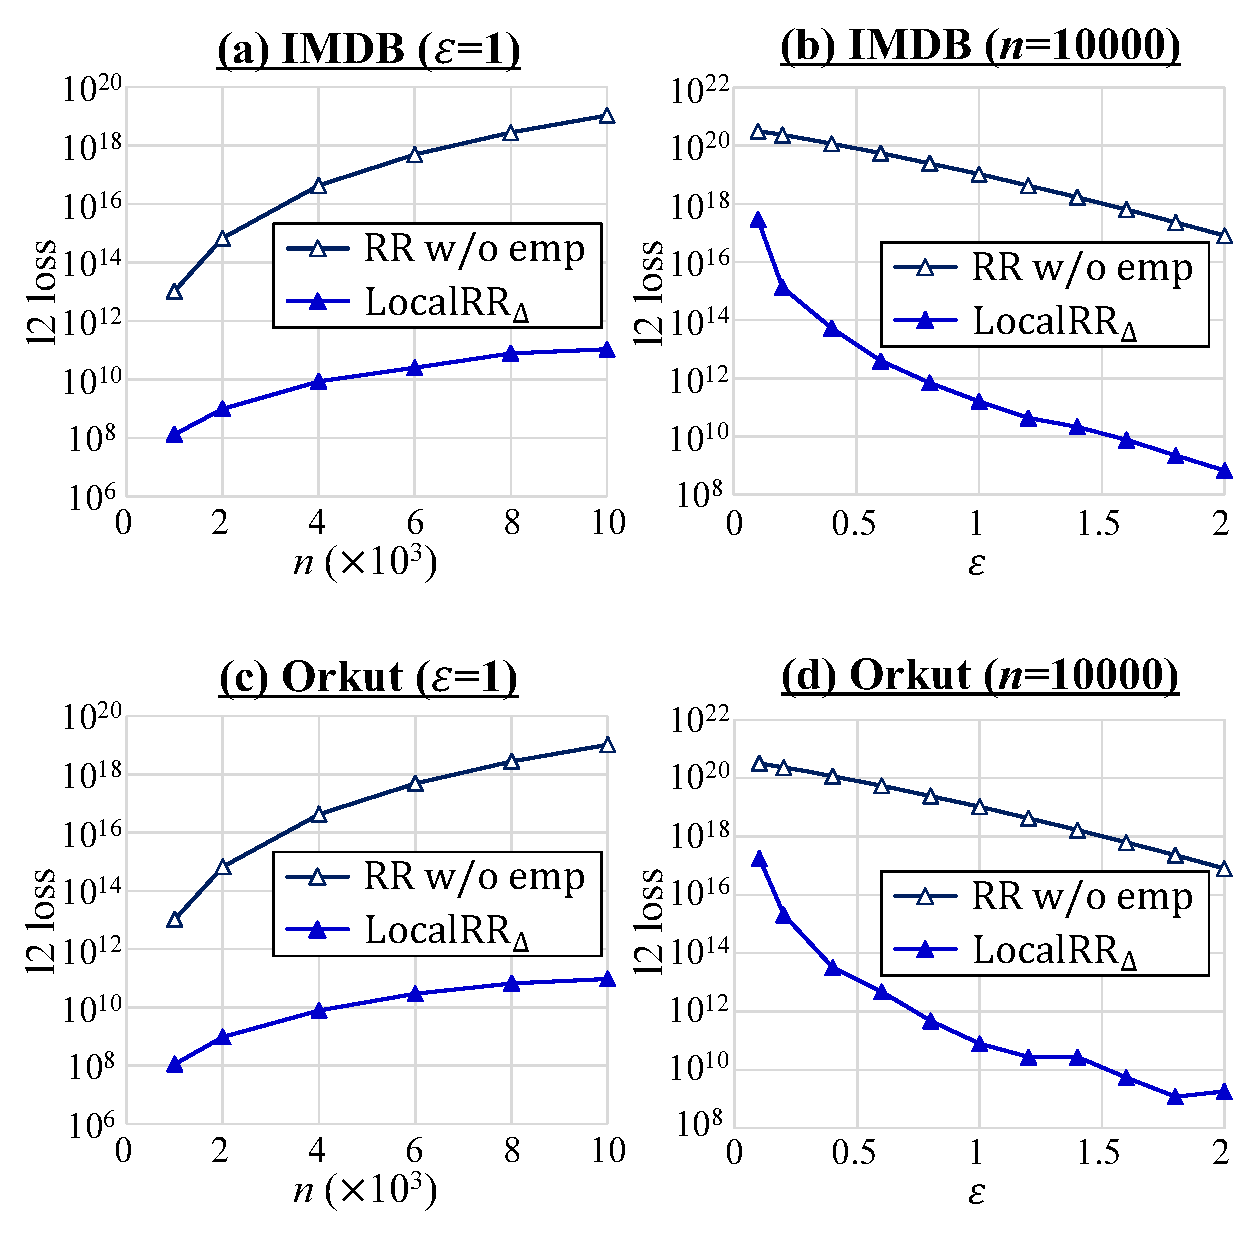
\includegraphics[width=0.99\linewidth]{fig/res5_RR_wo_emp.pdf}
\vspace{-5mm}
\caption{$l_2$ loss of \alg{LocalRR$_\triangle$} and the RR without empirical estimation (\alg{RR w/o emp}).}
\label{fig:res5_RR_wo_emp}
\end{figure}

\section{Experiments on Barab\'{a}si-Albert Graphs}
\label{sec:BAGraph}
% \smallskip
\noindent{\textbf{Experimental set-up.}}~~In Section~\ref{sec:experiments}, we evaluated our algorithms using two real datasets: \IMDB{} and \Orkut{}. 
We also evaluated our algorithms using artificial graphs that have power-law degree distributions. 
% based on 
We used the BA (Barab\'{a}si-Albert) model \cite{NetworkScience} to generate such graphs.

In the BA model, an artificial graph (referred to as a BA graph)
% of $n$ nodes 
is grown by adding new nodes one at a time. 
Each new node is connected to $\lambda \in \nats$ existing nodes with probability proportional to the degree of the existing node. 
% the number of edges that the existing nodes have. 
In our experiments, we used 
NetworkX \cite{Hagberg_SciPy08}, a Python package for graph analysis, to generate BA graphs.

We generated a BA graph $G^*$ with $1000000$ nodes using NetworkX. 
For the attachment parameter $\lambda$, we set $\lambda=10$ or $50$. 
When $\lambda=10$ (resp.~$50$), the average degree of $G^*$ was $10.0$ (resp.~$50.0$). 
For each case, we randomly generated $n$ users from the whole graph $G^*$, and extracted a graph $G=(V,E)$ with the $n$ users. 
Then we estimated the number of triangles $f_\triangle(G)$ and the number of $2$-stars $f_{2\star}(G)$. 
For triangles, we evaluated \alg{LocalRR$_\triangle$}, \alg{Local2Rounds$_\triangle$}, and \alg{CentralLap$\triangle$}. 
For $2$-stars, we evaluated \alg{LocalLap$_2\star$} and \alg{CentralLap$_2\star$}. 
In \alg{Local2Rounds$_\triangle$}, we set $\epsilon_1 = \epsilon_2$.
For $\td_{max}$, we set $\td_{max} = d_{max}$. 

We evaluated the $l_2$ loss while changing $n$ and $\epsilon$. 
We attempted $\gamma \in \nats$ ways to randomly select $n$ users from $G^*$, and averaged the $l_2$ loss over all the $\gamma$ ways to randomly select $n$ users. 
As with Section~\ref{sec:experiments}, we set $\gamma=100$ and changed $n$ from $1000$ to $10000$ while fixing $\epsilon=1$. 
Then we set $\gamma=10$ and changed $\epsilon$ from $0.1$ to $2$ while fixing $n=10000$.
% When we changed $n$ from $1000$ to $10000$ while fixing $\epsilon=1$, we set $\gamma = 100$. 
% When we changed $\epsilon$ from $0.1$ to $2$ while fixing $n=10000$, we set $\gamma = 10$.

\smallskip
\noindent{\textbf{Experimental results.}}~~Figure~\ref{fig:res6_BAGraph} shows the results. 
Overall, Figure~\ref{fig:res6_BAGraph} has a similar tendency to Figures~\ref{fig:res1_n_l2loss_tri}, \ref{fig:res1_n_l2loss_kst}, and \ref{fig:res2_eps_l2loss}. 
For example, \alg{Local2Rounds$_\triangle$} significantly outperforms \alg{LocalRR$_\triangle$}, especially when the graph $G$ is sparse; i.e., $\lambda = 10$. 
In \alg{Local2Rounds$_\triangle$}, \alg{CentralLap$\triangle$}, \alg{LocalLap$_2\star$}, and \alg{CentralLap$_2\star$}, the $l_2$ loss increases with increase in $\lambda$. 
This is because the maximum degree $d_{max}$ $(= \td_{max})$ increases with increase in $\lambda$.

\begin{figure}[t]
\centering
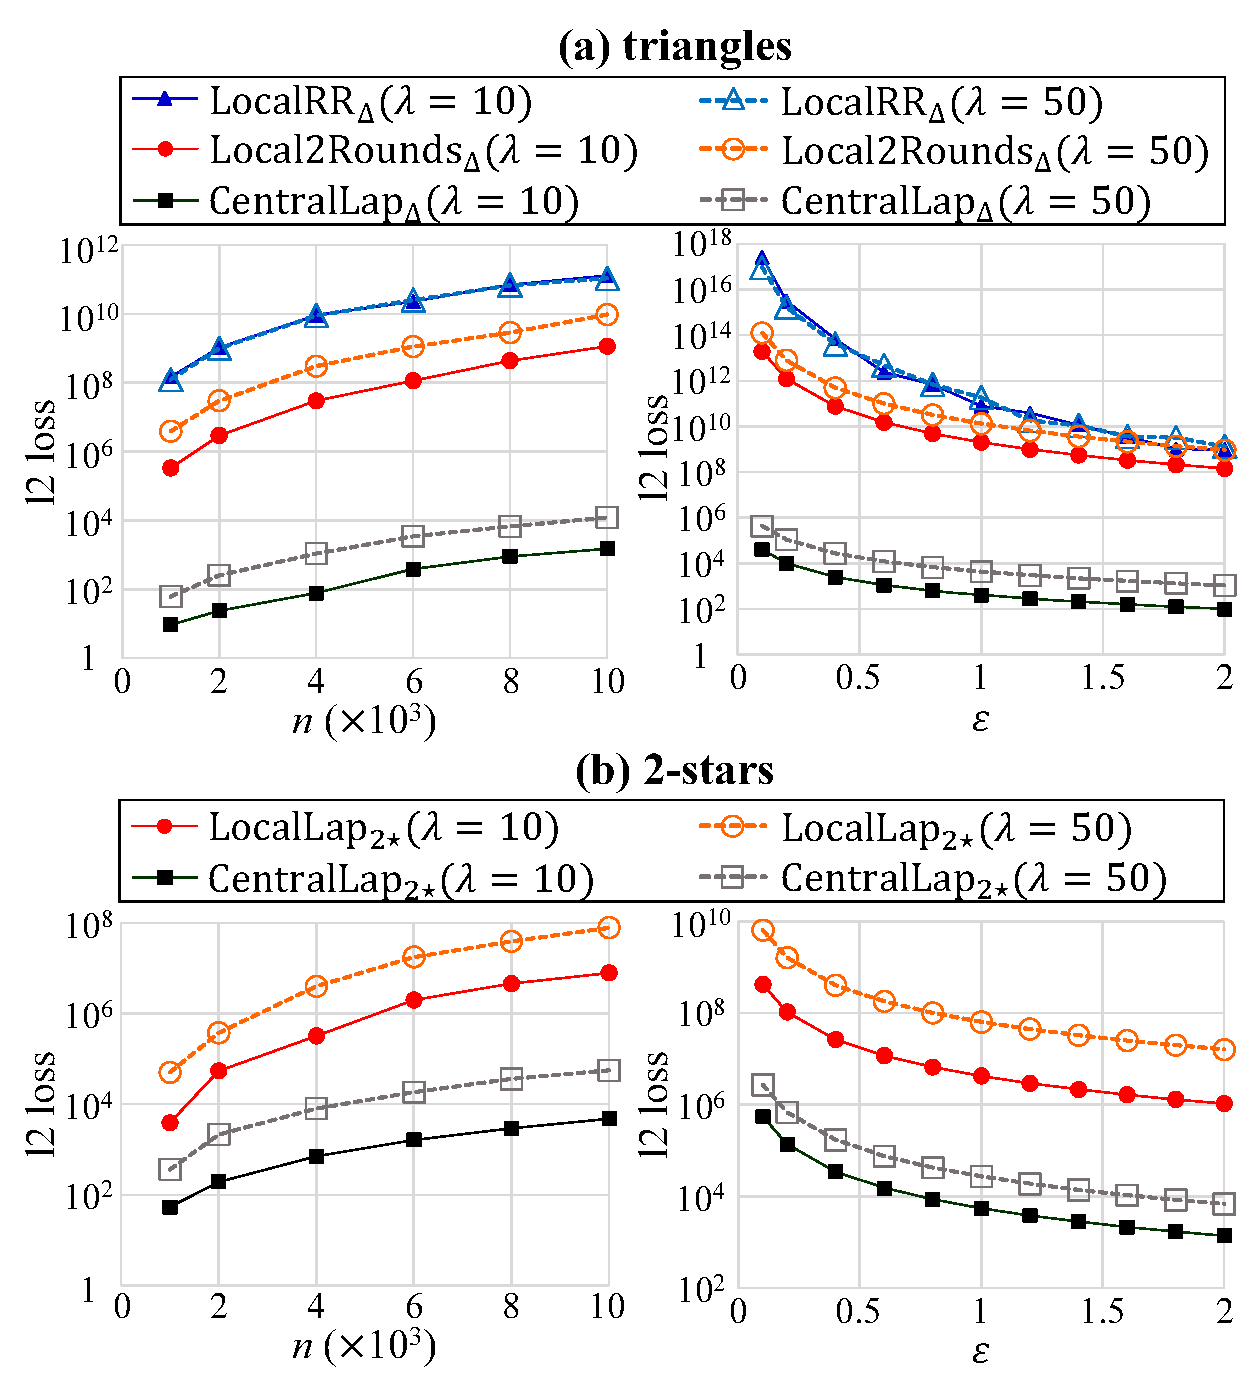
\includegraphics[width=0.99\linewidth]{fig/res6_BAGraph.pdf}
\vspace{-2mm}
\caption{$l_2$ loss in the Barab\'{a}si-Albert graph datasets 
% We set $\epsilon=1$ ($\epsilon_1 = \epsilon_2 = \frac{1}{2}$) in the left figures, and $n=10000$ in the right figures. 
(left: $\epsilon=1$, right: $n=10000$). 
We set the attachment parameter $\lambda$ in the BA model to $\lambda=10$ or $50$, and $\td_{max}$ to $\td_{max} = d_{max}$.}
\label{fig:res6_BAGraph}
\end{figure}

Figure~\ref{fig:res6_BAGraph} also shows that the $l_2$ loss is roughly consistent with our upper-bounds in Section~\ref{sec:algorithms}. 
For example, recall that \alg{LocalRR$_\triangle$}, \alg{Local2Rounds$_\triangle$}, \alg{CentralLap$_\triangle$}, \alg{LocalLap$_{2\star}$}, and \alg{CentralLap$_{2\star}$} achieve the expected $l_2$ loss of $O(n^4)$, $O(nd_{max}^3)$, $O(d_{max}^2)$, $O(nd_{max}^{2})$, and $O(d_{max}^{2})$, respectively. 
Assuming that $d_{max} = O(n)$, the left panels of Figure~\ref{fig:res6_BAGraph} are roughly consistent with these upper-bounds. 
In addition, the right panels of Figure~\ref{fig:res6_BAGraph} show that when we set $\lambda=10$ and decrease $\epsilon$ from $0.4$ to $0.1$, the $l_2$ loss increases by a factor of about $3800$, $250$, and $16$ in \alg{LocalRR$_\triangle$}, \alg{Local2Rounds$_\triangle$}, and \alg{CentralLap$_\triangle$}, respectively. 
They are roughly consistent with our upper-bounds -- for small $\epsilon$, the expected $l_2$ loss of \alg{LocalRR$_\triangle$}, \alg{Local2Rounds$_\triangle$}, and \alg{CentralLap$_\triangle$} is  $O(\epsilon^{-6})$, $O(\epsilon^{-4})$, and $O(\epsilon^{-2})$, respectively.

In summary, for both the two real datasets and the BA graphs, our experimental results showed the following findings: 
(1) \alg{Local2Rounds$_\triangle$} significantly outperforms \alg{LocalRR$_\triangle$}, especially when the graph $G$ is sparse; 
(2) our experimental results are roughly consistent with our upper-bounds.

% \subsection{Construction of an $(n, \frac{d_{max}}{2}-2)$ independent cube for $f_\triangle$}
\section{Construction of an $(n, \frac{d_{max}}{2}-2)$ independent cube for $f_\triangle$}
\label{sub:cube_triangle}
Suppose that $n$ is even and $d_{max}$ is divisible by $4$.
Since $d_{max} < n$, it is possible to write 
% $n = k \frac{d_{max}}{2} + r$ 
$n = \eta_1 \frac{d_{max}}{2} + \eta_2$ 
for integers 
% $k,r$ 
$\eta_1, \eta_2$
such that 
% $k \geq 1$ and $1 \leq r < \frac{d_{max}}{2}$. 
$\eta_1 \geq 1$ and $1 \leq \eta_2 < \frac{d_{max}}{2}$. 
Because 
% $k \frac{d_{max}}{2}$ 
$\eta_1 \frac{d_{max}}{2}$ 
and $n$ are even, 
we must have 
% $r$ 
$\eta_2$ 
is even.
Now, we can write 
% $n = (k-1) \frac{d_{max}}{2} + (r+\frac{d_{max}}{2})$.
$n = (\eta_1-1) \frac{d_{max}}{2} + (\eta_2 + \frac{d_{max}}{2})$.
% This means 
Thus, 
we can define 
% the 
a graph $G=(V,E)$ on $n$ 
% vertices 
nodes 
consisting of 
% $(k-1)$ 
$(\eta_1-1)$ 
cliques of 
even 
size
$\frac{d_{max}}{2}$ and one final clique of an even size $\eta_2+\frac{d_{max}}{2} \in (\frac{d_{max}}{2}, d_{max})$ 
% between $\frac{d_{max}}{2}$ and $d_{max}$ 
with all cliques disjoint. 

Since $G=(V,E)$ consists of even-sized cliques, it contains a perfect matching $M$. 
Figure~\ref{fig:mono-cube_triangle} shows examples of $G$ and $M$, where $n=14$, $d_{max} = 8$, $\eta_1 = 3$, and $\eta_2 = 2$. 
Let 
% $G' = G \setminus M$. 
$G'=(V,E')$ such that $E' = E \setminus M$. 
Let $\calA = \{(V,E' \cup N: N \subseteq M\}$. 
Each edge in $G$ is part of at least $\frac{d_{max}}{2}-2$ triangles. 
For each pair of edges in $M$, the triangles of $G$ of which they are part
are disjoint. 
Thus, 
% for any $N \subseteq M$, with $e \in N$, 
for any edge $e \in M$, 
removing $e$ 
% $e \in N$
from 
% $G \setminus N$ 
a graph in $\calA$ 
will remove at least $\frac{d_{max}}{2}-2$ triangles. This implies 
that $\calA$ 
% $\calA = \{G \cup N : N \subseteq M\}$ 
is an $(n,\frac{d_{max}}{2}-2)$ independent cube for $f_\triangle$.

%Similarly, for even natural number $l \in \nats$ such that $d_{max}>l+2$, we can construct an $(n,d_{max}-l-2)$ independent cube from the adjacency matrix of a collection of cliques of size $d_{max}-l$.

\begin{figure}[t]
  \centering
  %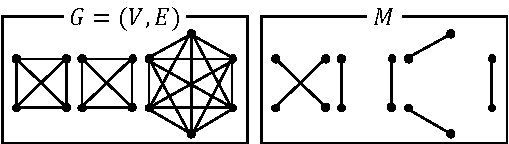
\includegraphics[width=0.88\linewidth]{fig/MonoCube_triangle.pdf}
  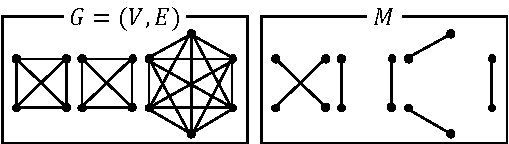
\includegraphics[width=0.88\linewidth]{fig/IndCube_triangle.pdf}
  \vspace{-2mm}
  \caption{
    Examples of $G$ and $M$ for constructing an independent cube for $f_\triangle$ ($n=14$, $d_{max} = 8$, $\eta_1 = 3$, $\eta_2 = 2$).
  }\label{fig:mono-cube_triangle}
\end{figure}


\arxiv{
\section{Proof of Statements in Section~\ref{sec:algorithms}}
\label{sec:proof}
Here we prove the statements in Section~\ref{sec:algorithms}. 
Our proofs will repeatedly use the well-known bias-variance decomposition \cite{mlpp}, which we briefly explain below. 
We denote the variance of the random variable $X$ by $\mathbb{V}[X]$. 
If we are producing a private, randomized estimate $\hat{f}(G)$ of the graph function $f(G)$, then the expected $l_2$ loss (over the randomness in the algorithm) can be written as: 
\begin{equation}\label{eq:bias-var}
  \E[l_2^2(\hat{f}(G),f(G))] = \left(\E[\hat{f}(G)] - f(G)\right)^2
  + \V[\hat{f}(G)].
\end{equation}
The first term is the bias, and the second term is the variance. 
If the estimate is unbiased (i.e., $\E[\hat{f}(G)] = f(G)$), then the expected $l_2$ loss is equal to the variance.

\subsection{Proof of Theorem~\ref{thm:k-stars_LDP}}
Let $\calR_i$ be \alg{LocalLap$_{k\star}$}. 
Let $d_i,d'_i \in \nnints$ be the number of ``1''s in two neighbor lists $\bma_i,\bma'_i \in \{0,1\}^n$ that differ in one bit. 
% Consider two neighbor lists $\bma_i,\bma'_i \in \{0,1\}^n$ that differ in one bit. 
% Let $d_i$ (resp.~$d'_i$) $\in \nnints$ be the number of ``1''s in $\bma_i$ (resp.~$\bma'_i$). 
Let $r_i = \binom{d_i}{k}$ and $r'_i = \binom{d'_i}{k}$. 
Below we consider two cases about $d_i$: when $d_i < \td_{max}$ and when $d_i \geq \td_{max}$.

\smallskip
\noindent{\textbf{Case 1: $d_i < \td_{max}$.}}~~In this case, both $\bma_i$ and $\bma'_i$ do not change after graph projection, as $d'_i \leq d_i + 1 \leq \td_{max}$. 
Then we obtain:
\begin{align*}
\Pr[\calR_i(\bma_i) = \hr_i] &= \exp\left(-\frac{\epsilon |\hr_i- r_i|}{\Delta}\right) \\
\Pr[\calR_i(\bma'_i) = \hr_i] &= \exp\left(-\frac{\epsilon |\hr_i- r'_i|}{\Delta}\right),
\end{align*}
where $\Delta = \binom{\td_{max}}{k-1}$. 
Therefore, 
% and hence 
\begin{align}
\frac{\Pr[\calR_i(\bma_i) = \hr_i]}{\Pr[\calR_i(\bma'_i) = \hr_i]} 
&= \exp\left( \frac{\epsilon |\hr_i- r'_i|}{\Delta} - \frac{\epsilon |\hr_i- r_i|}{\Delta}\right) \nonumber\\
&\leq  \exp\left( \frac{\epsilon |r'_i- r_i|}{\Delta} \right) \label{eq:Pr_R_i_a'_i_a_i}\\
& \hspace{4mm} (\text{by the triangle inequality}). \nonumber
\end{align}
If $d'_i = d_i + 1$, then $|r'_i- r_i|$ in (\ref{eq:Pr_R_i_a'_i_a_i}) can be written as follows:
\begin{align*}
|r'_i- r_i| 
= \binom{d_i+1}{k} - \binom{d_i}{k} 
= \binom{d_i}{k-1}
< \binom{\td_{max}}{k-1}
= \Delta, 
\end{align*}
Since we add $\Lap(\frac{\Delta}{\epsilon})$ to $r_i$, we obtain:
\begin{align}
\Pr[\calR_i(\bma_i) = \hr_i] \leq e^\epsilon \Pr[\calR_i(\bma'_i) = \hr_i]. 
\label{eq:R_i_a_i_hr_i}
\end{align}
If $d'_i = d_i - 1$, then $|r'_i- r_i| = \binom{d_i}{k} - \binom{d_i-1}{k} = \binom{d_i-1}{k-1} < \Delta$ and (\ref{eq:R_i_a_i_hr_i}) holds. 
Therefore, \alg{LocalLap$_{k\star}$} provides $\epsilon$-edge LDP. 

\smallskip
\noindent{\textbf{Case 2: $d_i \geq \td_{max}$.}}~~Assume 
% Second, we consider the case where $d_i \geq \td_{max}$. 
that $d'_i = d_i + 1$. 
In this case, $d'_i > \td_{max}$. 
Therefore, $d'_i$ becomes $\td_{max}$ after graph projection. 
In addition, 
% If $d_i > \td_{max}$, then 
$d_i$ also becomes $\td_{max}$ after graph projection. 
Therefore, we obtain 
$d_i = d'_i = \td_{max}$ after graph projection. 
Thus 
% and $r_i = r'_i = \binom{\td_{max}}{k}$. 
% Therefore, 
$\Pr[\calR_i(\bma_i) = \hr_i] = \Pr[\calR_i(\bma'_i) = \hr_i]$. 

Assume that $d'_i = d_i - 1$. 
If $d_i > \td_{max}$, then $d_i = d'_i = \td_{max}$ after graph projection. 
Thus $\Pr[\calR_i(\bma_i) = \hr_i] = \Pr[\calR_i(\bma'_i) = \hr_i]$. 
If $d_i = \td_{max}$, then (\ref{eq:R_i_a_i_hr_i}) holds. 
Therefore, \alg{LocalLap$_{k\star}$} provides $\epsilon$-edge LDP. \qed

\subsection{Proof of Theorem~\ref{thm:k-stars}}
Assuming the maximum degree $d_{max}$ of $G$ is at most $\td_{max}$, the only
randomness in the algorithm will be the Laplace noise since graph projection
will not occur.
Since the Laplacian noise $\Lap(\frac{\Delta}{\epsilon})$ has mean $0$, the estimate $\hf_{k\star}(G, \epsilon, \td_{max})$ is unbiased. 
Then by the bias-variance decomposition \cite{mlpp}, 
the expected $l_2$ loss 
$\mathbb{E}[l_2^2(\hf_{k\star}(G, \epsilon, \td_{max}),\allowbreak f_{k\star}(G))]$ is equal to the variance of $\hf_{k\star}(G, \epsilon, \td_{max})$. 
% We denote the variance of the random variable $X$ by $\mathbb{V}[X]$. 
The variance of $\hf_{k\star}(G, \epsilon, \td_{max})$ can be written as follows:
\begin{align*}
    \mathbb{V}[\hf_{k\star}(G, \epsilon, \td_{max})] 
    &= \mathbb{V}\left[ \sum_{i=1}^n \Lap\left( \frac{\Delta}{\epsilon} \right) \right] \\
    &= \frac{n \Delta^2}{\epsilon^2}.
\end{align*}
% Note that $\tilde{m}_3$ and $\tilde{m}_0$ are not dependent. 
Since $\Delta = \binom{\td_{max}}{k-1} = O(\td_{max}^{k-1})$, we obtain:
\begin{align*}
    \mathbb{E}[l_2^2(\hf_{k\star}(G, \epsilon, \td_{max}), f_{k\star}(G))] 
    &= \mathbb{V}[\hf_{k\star}(G, \epsilon, \td_{max})] \\
    &= O\left(\frac{n \td_{max}^{2k-2}}{\epsilon^2}\right).
\end{align*}
\qed

\subsection{Proof of Proposition~\ref{prop:triangle_emp}}
Let $\mu = e^\epsilon$ and $\bmQ \in [0,1]^{4 \times 4}$ be a $4 \times 4$ matrix such that:
\begin{align}
  \bmQ = \frac{1}{(\mu+1)^3} \left(
    \begin{array}{cccc}
      \mu^3 & 3\mu^2 & 3\mu & 1 \\
      \mu^2 & \mu^3+2\mu & 2\mu^2+1 & \mu \\
      \mu & 2\mu^2+1 & \mu^3+2\mu & \mu^2 \\
      1 & 3\mu & 3\mu^2 & \mu^3
    \end{array}
  \right).
  \label{eq:Q_1}
\end{align}
Let $c_3, c_2, c_1, c_0 \in \nnints$ be respectively the number of triangles, 2-edges, 1-edge, and no-edges in $G$. 
Then we obtain:
\begin{align}
(\mathbb{E}[m_3], \mathbb{E}[m_2], \mathbb{E}[m_1],
\mathbb{E}[m_0]) = (c_3, c_2, c_1, c_0) \bmQ.
\label{eq:bmQ}
\end{align}
In other words, $\bmQ$ is a transition matrix from a type of subgraph (i.e., triangle, 2-edges, 1-edge, or no-edge) in $G$ to a type of subgraph in $G'$. 

Let $\hat{c}_3, \hat{c}_2, \hat{c}_1, \hat{c}_0 \in \reals$ be the empirical estimate of $(c_3, c_2, c_1, c_0)$. 
By (\ref{eq:bmQ}), they can be written as follows:
\begin{align}
(\hat{c}_3, \hat{c}_2, \hat{c}_1, \hat{c}_0) = (m_3, m_2, m_1, m_0) \bmQ^{-1}.
\label{eq:hc3_hc2_hc1_hc0}
\end{align}
Let $\bmQ_{i,j}^{-1}$ be the ($i,j$)-th element of $\bmQ^{-1}$. 
By using Cramer's rule, we obtain: 
\begin{align}
\bmQ_{1,1}^{-1} &= \textstyle{\frac{\mu^3}{(\mu-1)^3}},~ \bmQ_{2,1}^{-1} =  \textstyle{-\frac{\mu^2}{(\mu-1)^3}}, \label{eq:bmQ11_bmQ21}\\
\bmQ_{3,1}^{-1} &= \textstyle{\frac{\mu}{(\mu-1)^3}},~ \bmQ_{4,1}^{-1} = \textstyle{-\frac{1}{(\mu-1)^3}}.
\label{eq:bmQ31_bmQ41}
\end{align}
By (\ref{eq:hc3_hc2_hc1_hc0}), (\ref{eq:bmQ11_bmQ21}), and (\ref{eq:bmQ31_bmQ41}), we obtain:
\begin{align*}
\textstyle{\hat{c}_3 = \frac{\mu^3}{(\mu-1)^3} m_3 - \frac{\mu^2}{(\mu-1)^3} m_2 + \frac{\mu}{(\mu-1)^3} m_1 - \frac{1}{(\mu-1)^3} m_0.}
\end{align*}
Since $\mu = e^\epsilon$ and the empirical estimate is unbiased \cite{Kairouz_ICML16,Wang_USENIX17}, we obtain (\ref{eq:triangle_emp}) in Proposition~\ref{prop:triangle_emp}. \qed

\subsection{Proof of Theorem~\ref{thm:subgraph-rr_LDP}}
Since \alg{LocalRR$_\triangle$} applies the RR to the lower triangular part of the adjacency matrix $\bmA$, it provides $\epsilon$-edge LDP for $(R_1, \ldots, R_n)$. 
Lines 5 to 8 in Algorithm~\ref{alg:subgraph-rr} are post-processing of $(R_1, \ldots, R_n)$. 
Thus, by the immunity to post-processing \cite{DP}, \alg{LocalRR$_\triangle$} provides $\epsilon$-edge LDP for the output $\frac{1}{(\mu-1)^3}(\mu^3 m_3 -\mu^2 m_2 + \mu m_1 - m_0)$. 

In addition, the existence of edge $(v_i,v_j) \in E$ $(i>j)$ affects only one element $a_{i,j}$ in the lower triangular part of $\bmA$. 
Therefore, \alg{LocalRR$_\triangle$} provides $\epsilon$-relationship DP.

\subsection{Proof of Theorem~\ref{thm:subgraph-rr}}
\label{sub:proof_thm:subgraph-rr}
By Proposition~\ref{prop:triangle_emp}, the estimate $\hf_{\triangle}(G, \epsilon)$ by \alg{LocalRR$_\triangle$} is unbiased. 
Then by the bias-variance decomposition \cite{mlpp}, 
the expected $l_2$ loss $\mathbb{E}[l_2^2(\hf_{\triangle}(G, \epsilon), f_\triangle(G))]$ is equal to the variance of $\hf_{\triangle}(G, \epsilon)$. 
% We denote the variance of the random variable $X$ by $\mathbb{V}[X]$. 
Let 
$a_3 = \frac{\mu^3}{(\mu-1)^3}$, 
$a_2 = - \frac{\mu^2}{(\mu-1)^3}$, 
$a_1 = \frac{\mu}{(\mu-1)^3}$, and 
$a_0 = - \frac{1}{(\mu-1)^3}$. 
Then the variance of $\hf_{\triangle}(G, \epsilon)$ can be written as follows:
\begin{align}
    \V[\hf_{\triangle}(G, \epsilon)] 
    &= \V[a_3 m_3 + a_2 m_2 + a_1 m_1 + a_0 m_0] \nonumber\\
    &= a_3^2 \V[m_3] + a_2^2 \V_{RR}[m_2] + a_1^2 \V[m_1] + a_0^2 \V[m_0] \nonumber\\
    &\hspace{3.5mm} + \sum_{i=0}^3 \sum_{j=0, j \ne i}^3 2a_i a_j \text{cov}(m_i, m_j),
    \label{eq:V_a3m3_a2m2_a1m1_a0m0}
\end{align}
where $\text{cov}(m_i, m_j)$ represents the covariance of $m_i$ and $m_j$. 
The covariance $\text{cov}(m_i, m_j)$ can be written as follows:
\begin{align}
    \text{cov}(m_i, m_j)
    &\leq \sqrt{\V[m_i] \V[m_j]} \nonumber\\
    &\hspace{4.2mm} (\text{by Cauchy-Schwarz inequality}) \nonumber\\
    &\leq  \max\{ \V[m_i], \V[m_j]\} \nonumber\\
    &\leq \V[m_i] + \V[m_j].
    \label{eq:cov_mi_mj}
\end{align}
By (\ref{eq:V_a3m3_a2m2_a1m1_a0m0}) and (\ref{eq:cov_mi_mj}), we obtain:
\begin{align}
    &\V[\hf_{\triangle}(G, \epsilon)] \nonumber\\
    &\leq (a_3^2 + 4a_3(a_2 + a_1 + a_0)) \V[m_3] \nonumber\\
    & \hspace{4.5mm} + (a_2^2 + 4a_2(a_3 + a_1 + a_0)) \V[m_2] \nonumber\\
    & \hspace{4.5mm} + (a_1^2 + 4a_1(a_3 + a_2 + a_0)) \V[m_1] \nonumber\\
    & \hspace{4.5mm} + (a_0^2 + 4a_0(a_3 + a_2 + a_1)) \V[m_0] \nonumber\\
    &= O\left( \frac{e^{6\epsilon}}{(e^\epsilon-1)^6} (\V[m_3] + \V[m_2] + \V[m_1] + \V[m_0]) \right).
    % &\leq O\left(\frac{e^{6\epsilon}}{(e^\epsilon-1)^6} \V[m_3] + \frac{e^{5\epsilon}}{(e^\epsilon-1)^6}\V[m_2]
    % \right. \nonumber\\
    % & \hspace{10mm} \left. + \frac{e^{4\epsilon}}{(e^\epsilon-1)^6}\V[m_1] + \frac{e^{3\epsilon}}{(e^\epsilon-1)^6}\V[m_0]\right).
    \label{V_RR_m_3}
\end{align}

Below we calculate $\V[m_3]$, $\V[m_2]$, $\V[m_1]$, and $\V[m_0]$ by assuming the Erd\"{o}s-R\'{e}nyi model $\bmG(n, \alpha)$ for $G$:

\begin{lemma}\label{lem:erdos-renyi-variance}
  Let $G \sim \textbf{G}(n,\alpha)$. 
  %with $\alpha < \frac{1}{2}$. 
  Let $p = \frac{1}{e^\epsilon+1}$ and 
  $\beta = \alpha(1-p) + (1-\alpha)p$. 
  Then $\V[m_3] = O(\beta^5 n^4 + \beta^3
  n^3)$, $\V[m_2] = O(\beta^3 n^4 + \beta^2 n^3)$, and 
  $\V[m_1] = \V[m_0] = O(\beta n^4)$.
\end{lemma}
% We prove Lemma~\ref{lem:erdos-renyi-variance} at the end of Appendix~\ref{sub:proof_thm:subgraph-rr}. 
Before going into the proof of Lemma~\ref{lem:erdos-renyi-variance}, we prove Theorem~\ref{thm:subgraph-rr} using Lemma~\ref{lem:erdos-renyi-variance}. 
By (\ref{V_RR_m_3}) and Lemma~\ref{lem:erdos-renyi-variance}, we obtain: 
\begin{align*}
\V[\hf_{\triangle}(G, \epsilon)] = O\left( \frac{e^{6\epsilon}}{(e^\epsilon-1)^6} \beta n^4 \right),
\end{align*}
which proves Theorem~\ref{thm:subgraph-rr}. \qed

We now prove Lemma~\ref{lem:erdos-renyi-variance}:

\begin{proof}[Proof of Lemma~\ref{lem:erdos-renyi-variance}]
Fist we show the variance of $m_3$ and $m_0$. 
Then we show the variance of $m_2$ and $m_1$.

\smallskip
\noindent{\textbf{Variance of $m_3$ and $m_0$.}}~~Since each edge in the original graph $G$ is independently generated with probability $\alpha \in [0,1]$, each edge in the noisy graph $G'$ is independently generated with probability $\beta = \alpha (1-p) + (1 - \alpha) p \in [0,1]$, where $p=\frac{1}{e^\epsilon+1}$. 
Thus $m_3$ is the number of triangles in graph $G' \sim \textbf{G}(n,\beta)$.

For $i,j,k \in [n]$, let $y_{i,j,k} \in \{0,1\}$ be a variable that takes $1$ if and only if 
$(v_i, v_j, v_k)$ forms a triangle. 
Then $\mathbb{E}[m_3^2]$ can be written as follows:
\begin{align}
  \mathbb{E}[m_3^2] = \sum_{i<j<k} ~ \sum_{i'<j'<k'}
  \mathbb{E}[y_{i,j,k} y_{i',j',k'}] 
  \label{eq:E_RR_tm3}
\end{align}
$\mathbb{E}[y_{i,j,k} y_{i',j',k'}]$ in (\ref{eq:E_RR_tm3}) is the probability that both $(v_i,v_j,v_k)$ and $(v_{i'},v_{j'},v_{k'})$ form a triangle. 
This event can be divided into the following four types:
\begin{enumerate}
\item $(i,j,k)=(i',j',k')$. There are $\binom{n}{3}$ such terms in (\ref{eq:E_RR_tm3}). 
For each term, $\mathbb{E}[y_{i,j,k} y_{i',j',k'}] = \beta^3$.
\item $(i,j,k)$ and $(i',j',k')$ have two elements in common. 
There are $\binom{n}{2} (n-2) (n-3) = 12\binom{n}{4}$ such terms in (\ref{eq:E_RR_tm3}). 
For each term, $\mathbb{E}[y_{i,j,k} y_{i',j',k'}] = \beta^5$. 
\item $(i,j,k)$ and $(i',j',k')$ have one element in common. 
There are $n \binom{n-1}{2} \binom{n-3}{2} = 30\binom{n}{5}$ such terms in (\ref{eq:E_RR_tm3}). 
For each term, $\mathbb{E}[y_{i,j,k} y_{i',j',k'}] = \beta^6$. 
\item $(i,j,k)$ and $(i',j',k')$ have no common elements. 
There are $\binom{n}{3} \binom{n-3}{3} = 20\binom{n}{6}$ such terms in in (\ref{eq:E_RR_tm3}). 
For each term, $\mathbb{E}[y_{i,j,k} y_{i',j',k'}] = \beta^6$. 
\end{enumerate}
Moreover, $\mathbb{E}[m_3]^2 = \binom{n}{3}^2 \beta^6$. 
Therefore, the variance of $m_3$ can be written as follows:
\begin{align*}
    \V[m_3] 
    &= \textstyle{\binom{n}{3} \beta^3 + 12\binom{n}{4} \beta^5 + 30\binom{n}{5} \beta^6 + 20\binom{n}{6} \beta^6 - \binom{n}{3}^2 \beta^6} \\
    &= \textstyle{\binom{n}{3} \beta^3 (1-\beta^3) + 12\binom{n}{4}\beta^5(1-\beta)} \\
    &= O(\beta^5 n^4 + \beta^3 n^3).
\end{align*}

By changing $\beta$ to $1-\beta$ and counting triangles, we get a random variable with the same distribution as $m_0$. Thus,
\begin{align*}
  \V[m_0] 
  &= \textstyle{\binom{n}{3} (1-\beta)^3(1-(1-\beta)^3) + 12\binom{n}{4} (1-\beta)^5\beta}
  \\
  &= O(\beta n^4).
\end{align*}
\smallskip
\noindent{\textbf{Variance of $m_2$ and $m_1$.}}~~For $i,j,k \in [n]$, let $z_{i,j,k} \in \{0,1\}$ be a variable that takes $1$ if and only if 
$(v_i, v_j, v_k)$ forms $2$-edges (i.e., exactly one edge is missing in the three nodes). 
Then $\mathbb{E}[m_2^2]$ can be written as follows:
\begin{align}
  \mathbb{E}[m_2^2] = \sum_{i<j<k} \sum_{i'<j'<k'}
  \mathbb{E}[z_{i,j,k} z_{i',j',k'}] 
  \label{eq:E_RR_tm2}
\end{align}
$\mathbb{E}[z_{i,j,k} z_{i',j',k'}]$ in (\ref{eq:E_RR_tm2}) is the probability that both $(v_i,v_j,v_k)$ and $(v_{i'},v_{j'},v_{k'})$ form $2$-edges. 
This event can be divided into the following four types:
\begin{enumerate}
	\item $(i,j,k)=(i',j',k')$. There are $\binom{n}{3}$ such terms in (\ref{eq:E_RR_tm2}). 
    For each term, $\mathbb{E}[z_{i,j,k} z_{i',j',k'}]=3\beta^2(1-\beta)$. 
	\item $(i,j,k)$ and $(i',j',k')$ have two elements in common. 
	There are $\binom{n}{2}(n-2)(n-3) = 12 \binom{n}{4}$ such terms in (\ref{eq:E_RR_tm2}). 
	For example, consider a term in which $i=i'=1$, $j=j'=2$, $k=3$, and $k'=4$. 
	Both $(v_1,v_2,v_3)$ and $(v_1,v_2,v_4)$ form 2-edges if:\\
	(a) $(v_1,v_2), (v_1,v_3), (v_1,v_4) \in E'$, $(v_2,v_3), (v_2,v_4) \notin E'$, \\
	(b) $(v_1,v_2), (v_1,v_3), (v_2,v_4) \in E'$, $(v_2,v_3), (v_1,v_4) \notin E'$, \\
	(c) $(v_1,v_2), (v_2,v_3), (v_1,v_4) \in E'$, $(v_1,v_3), (v_2,v_4) \notin E'$, \\
	(d) $(v_1,v_2), (v_2,v_3), (v_2,v_4) \in E'$, $(v_1,v_3), (v_1,v_4) \notin E'$, or \\
	(e) $(v_1,v_3), (v_1,v_4), (v_2,v_3), (v_2,v_4) \in E'$, $(v_1,v_2) \notin E'$. \\
    Thus, $\mathbb{E}[z_{i,j,k} z_{i',j',k'}]=4\beta^3(1-\beta)^2 + \beta^4(1-\beta)$ for this term. 
    Similarly, $\mathbb{E}[z_{i,j,k} z_{i',j',k'}]=4\beta^3(1-\beta)^2 + \beta^4(1-\beta)$ for the other terms.
	\item $(i,j,k)$ and $(i',j',k')$ have one element in common. 
	There are $n \binom{n-1}{2} \binom{n-3}{2} = 30\binom{n}{5}$ such terms in (\ref{eq:E_RR_tm2}).  For each term, $\mathbb{E}[z_{i,j,k}z_{i',j',k'}]=(3\beta^2(1-\beta))^2 = 9\beta^4(1-\beta)^2$. 
	\item $(i,j,k)$ and $(i',j',k')$ have no common elements. 
	There are $\binom{n}{3}\binom{n-3}{3} = 20\binom{n}{6}$ such terms in (\ref{eq:E_RR_tm2}). 
	For each term, $\mathbb{E}[z_{i,j,k}z_{i',j',k'}]=(3\beta^2(1-\beta))^2 = 9\beta^4(1-\beta)^2$. 
\end{enumerate}
Moreover, $\mathbb{E}[m_2]^2 = (3\binom{n}{3}\beta^2(1-\beta))^2 = 9\binom{n}{3}^2\beta^4(1-\beta)^2$. 
Therefore, the variance of $m_2$ can be written as follows:
\begin{align*}
  \mathbb{V}[m_2] 
  &= \mathbb{E}[m_2^2] - \mathbb{E}[m_2]^2 \nonumber\\
  &= \textstyle{3\binom{n}{3}\beta^2(1-\beta) + 12\binom{n}{4}\left(4\beta^3(1-\beta)^2 + \beta^4(1-\beta)\right)} \nonumber\\
  &\hspace{3.5mm} \textstyle{+ 270\binom{n}{5}\beta^4(1-\beta)^2 + 180\binom{n}{6}\beta^4(1-\beta)^2} \nonumber\\
  &\hspace{3.5mm} \textstyle{- 9\binom{n}{3}^2\beta^4(1-\beta)^2.}
\end{align*}
By simple calculations,
\begin{align*}
\textstyle{270\binom{n}{5} + 180\binom{n}{6} - 9\binom{n}{3}^2 = -108\binom{n}{4}-9\binom{n}{3}.}
\end{align*}
Thus we obtain:
\begin{align*}
\mathbb{V}[m_2] 
&= \textstyle{3\binom{n}{3}\beta^2(1-\beta)\left(1 - 3\beta^2(1-\beta)\right)} \nonumber\\
%&\hspace{3.5mm} \textstyle{+ 12\binom{n}{4}\left(4\beta^3(1-\beta)^2 + \beta^4(1-\beta) - 9\beta(1-\beta) \right)} \\
&\hspace{3.5mm} \textstyle{+ 12\binom{n}{4} \beta^3(1-\beta) \left(4(1-\beta) + \beta - 9\beta(1-\beta) \right)} \\
&= O(\beta^3 n^4 + \beta^2n^3).
\end{align*}
Similarly, the variance of $m_1$ can be written as follows:
\begin{align*}
\mathbb{V}[m_1] 
&= \textstyle{3\binom{n}{3}\beta(1-\beta)^2\left(1 - 3\beta(1-\beta)^2\right)} \nonumber\\
&\hspace{3.5mm} \textstyle{+ 12\binom{n}{4} \beta(1-\beta)^3 \left(4\beta +
(1-\beta) - 9\beta(1-\beta) \right)} \\
&= O(\beta n^4).
\end{align*}
\end{proof}

\subsection{Proof of Proposition~\ref{prop:triangle_emp_2rounds}}
Let $t_* = \sum_{i=1}^n t_i$ and $s_* = \sum_{i=1}^n s_i$. 
Let $s_*^{\wedge}$ be the number of triplets $(v_i,v_j,v_k)$ such that $j<k<i$, $a_{i,j} = a_{i,k} = 1$, and $a_{j,k} = 0$. 
Let $s_*^{\triangle}$ be the number of triplets $(v_i,v_j,v_k)$ such that $j<k<i$, $a_{i,j} = a_{i,k} = a_{j,k} =1$. 
Note that 
$s_* = s_*^{\wedge} + s_*^{\triangle}$ and 
$s_*^{\triangle} = f_\triangle(G)$. 

Consider a triangle $(v_i,v_j,v_k) \in G$. 
This triangle is counted $1-p_1$ ($= \frac{e^{\epsilon_1}}{e^{\epsilon_1}+1}$) times in expectation in $t_*$. 
Consider $2$-edges $(v_i,v_j,v_k) \in G$ (i.e., exactly one edge is missing in the three nodes). 
This is counted $p_1$ ($= \frac{1}{e^{\epsilon_1}+1}$) times in expectation in $t_*$.  
No other events can change $t_*$. 
% Thus, with respect to the randomness in the graph $G'$,
Therefore, we obtain:
\begin{align*}
\mathbb{E}[t_*] = (1-p_1) s_*^{\triangle} + p_1 s_*^{\wedge}. 
\end{align*}
By $s_* = s_*^{\wedge} + s_*^{\triangle}$ and 
$s_*^{\triangle} = f_\triangle(G)$, we obtain:
\begin{align*}
\mathbb{E}\left[\sum_{i=1}^n w_i \right] 
&= \mathbb{E}\left[\sum_{i=1}^n (t_i - p_1 s_i) \right] \\
&= \mathbb{E}[t_* - p_1 s_*] \\
&= \mathbb{E}[t_*] - p_1 \mathbb{E}[s_*^{\wedge} + s_*^{\triangle}] \\
&= (1-p_1) s_*^{\triangle} + p_1 s_*^{\wedge} - p_1 (s_*^{\wedge} + s_*^{\triangle}) \\
&= (1 - 2 p_1) f_\triangle(G),
\end{align*}
hence 
\begin{align*}
\textstyle{\mathbb{E}\left[ \frac{1}{1-2p_1} \sum_{i=1}^n w_i \right] = f_\triangle(G).}
\end{align*}
\qed

\subsection{Proof of Theorem~\ref{thm:local2rounds_LDP}}
Let $\calR_i$ be \alg{Local2Rounds$_{\triangle}$}. 
Consider two neighbor lists $\bma_i,\bma'_i \in \{0,1\}^n$ that differ in one bit. 
Let $d_i$ (resp.~$d'_i$) $\in \nnints$ be the number of ``1''s in $\bma_i$ (resp.~$\bma'_i$). 
Let $\bbma_i$ (resp.~$\bbma'_i$) $\in \{0,1\}^n$ be neighbor lists obtained by setting all of the $i$-th to the $n$-th elements in $\bma_i$ (resp.~$\bma'_i$) to $0$. 
Let $\bd_i$ (resp.~$\bd'_i$) $\in \nnints$ be the number of ``1''s in $\bbma_i$ (resp.~$\bbma'_i$). 
% from the first to the $(i-1)$-th elements in $\bma_i$ (resp.~$\bma'_i$). 
For example, if $n=6$, $\bma_4=(1,0,1,0,1,1)$, and $\bma'_4=(1,1,1,0,1,1)$, then 
$d_4=4$, $d'_4=5$, $\bbma_4=(1,0,1,0,0,0)$, $\bbma'_4=(1,1,1,0,0,0)$, $\bd_4=2$, and $\bd'_4=3$. 

Furthermore, 
let $t_i$ (resp.~$t'_i$) $\in \nnints$ be the number of triplets $(v_i, v_j, v_k)$ such that $j < k < i$, $(v_i,v_j) \in E$, $(v_i,v_k) \in E$, and $(v_j,v_k) \in E'$ in $\bma_i$ (resp.~$\bma'_i$). 
Let $s_i$ (resp.~$s'_i$) $\in \nnints$ be the number of triplets $(v_i, v_j, v_k)$ such that $j < k < i$, $(v_i,v_j) \in E$, and $(v_i,v_k) \in E$ in $\bma_i$ (resp.~$\bma'_i$). 
Let $w_i = t_i - p_1 s_i$ and $w'_i = t'_i - p_1 s'_i$. 
Below we consider two cases about $d_i$: when $d_i < \td_{max}$ and when $d_i \geq \td_{max}$. 

\smallskip
\noindent{\textbf{Case 1: $d_i < \td_{max}$.}}~~Assume that $d'_i = d_i + 1$. 
In this case, we have either $\bbma'_i = \bbma_i$ or $\bd'_i = \bd_i+1$. 
If $\bbma'_i = \bbma_i$, then $s_i = s'_i$, $t_i = t'_i$, and $w_i = w'_i$, hence $\Pr[\calR_i(\bma_i) = \hw_i] = \Pr[\calR_i(\bma'_i) = \hw_i]$. 
If $\bd'_i = \bd_i+1$, then $s_i$ and $s'_i$ can be expressed as $s_i = \binom{\bd_i}{2}$ and $s'_i = \binom{\bd'_i}{2} = \binom{\bd_i+1}{2}$, respectively. 
Then we obtain:
\begin{align*}
s'_i - s_i = \binom{\bd_i+1}{2} - \binom{\bd_i}{2} = \bd_i.
\end{align*}
In addition, since we consider an additional constraint ``$(v_j,v_k) \in E'$'' in counting $t_i$ and $t'_i$, 
we have $t'_i - t_i \leq s'_i - s_i$. 
Therefore, 
\begin{align*}
|w'_i - w_i| 
&= |t'_i - t_i - p_1 (s'_i - s_i)| \\
&\leq (1 - p_1) \bd_i \\
&\leq (1 - p_1) d_i \\
&< \td_{max} \hspace{5mm} \text{(by $p_1 > 0$ and $d_i < \td_{max}$)}.
\end{align*}
Since we add $\Lap(\frac{\td_{max}}{\epsilon_2})$ to $w_i$, we obtain:
\begin{align}
\Pr[\calR_i(\bma_i) = \hw_i] \leq e^{\epsilon_2} \Pr[\calR_i(\bma'_i) = \hw_i]. 
\label{eq:R_i_a_i_hr_i_2}
\end{align}

Assume that $d'_i = d_i - 1$. 
In this case, we have either $\bbma'_i = \bbma_i$ or $\bd'_i = \bd_i-1$. 
If $\bbma'_i = \bbma_i$, then $\Pr[\calR_i(\bma_i) = \hw_i] = \Pr[\calR_i(\bma'_i) = \hw_i]$. 
If $\bd'_i = \bd_i-1$, then we obtain $s_i - s'_i = \bd_i - 1$ and $t_i - t'_i \leq s_i - s'_i$. 
Thus $|w'_i - w_i| \leq (1-p_1) (\td_i - 1) < \td_{max}$ and (\ref{eq:R_i_a_i_hr_i_2}) holds. 
Therefore, \alg{Local2Rounds$_{\triangle}$} provides $\epsilon_2$-edge LDP at the second round. 
Since \alg{Local2Rounds$_{\triangle}$} provides $\epsilon_1$-edge LDP at the first round (by Theorem~\ref{thm:subgraph-rr_LDP}), it provides $(\epsilon_1 + \epsilon_2)$-edge LDP in total by the composition theorem \cite{DP}. 

\smallskip
\noindent{\textbf{Case 2: $d_i \geq \td_{max}$.}}~~Assume that $d'_i = d_i + 1$. 
In this case, we obtain $d_i = d'_i = \td_{max}$ after graph projection. 

Note that $\bma_i$ and $\bma'_i$ can differ in \textit{zero or two bits} after graph projection. 
For example, consider the case where $n=8$, $\bma_5=(1,1,0,1,0,1,1,1)$, $\bma'_5=(1,1,1,1,0,1,1,1)$, and $\td_{max}=4$. 
If the permutation is 1,4,6,8,2,7,5,3, then $\bma_5=\bma'_5=(1,0,0,1,0,1,0,1)$ after graph projection. 
However, if the permutation is 3,1,4,6,8,2,7,5, then $\bma_5$ and $\bma'_5$ become $\bma_5=(1,0,0,1,0,1,0,1)$ and $\bma'_5=(1,0,1,1,0,1,0,0)$, respectively; i.e., they differ in the third and eighth elements. 

If $\bma_i=\bma'_i$, then $\Pr[\calR_i(\bma_i) = \hw_i] = \Pr[\calR_i(\bma'_i) = \hw_i]$. 
If $\bma_i$ and $\bma'_i$ differ in two bits, $\bbma_i$ and $\bbma'_i$ differ in \textit{at most two bits} (because we set all of the $i$-th to the $n$-th elements in $\bma_i$ and $\bma'_i$ to $0$). 
For example, we can consider the following three cases:
\begin{itemize}
    \item If $\bma_5=(1,0,0,1,0,1,0,1)$ and $\bma'_5=(1,0,0,1,0,1,1,0)$, then $\bbma_5=\bbma'_5=(1,0,0,1,0,0,0,0)$. 
    \item If $\bma_5=(1,0,0,1,0,1,0,1)$ and $\bma'_5=(1,0,1,1,0,1,0,0)$, then $\bbma_5=(1,0,0,1,0,0,0,0)$ and $\bbma'_5=(1,0,1,1, 0,0,\allowbreak0,0)$; i.e., they differ in one bit. 
    \item If $\bma_5=(1,1,0,1,0,1,0,0)$ and $\bma'_5=(1,0,1,1,0,1,0,0)$, then $\bbma_5=(1,1,0,1,0,0,0,0)$ and $\bbma'_5=(1,0,1,1,0,0,\allowbreak0,0)$; i.e., they differ in two bits.
\end{itemize}
If $\bbma_i=\bbma'_i$, then $\Pr[\calR_i(\bma_i) = \hw_i] = \Pr[\calR_i(\bma'_i) = \hw_i]$. 
If $\bbma_i$ and $\bbma'_i$ differ in one bit, then $\bd'_i = \bd_i + 1$. 
In this case, we obtain (\ref{eq:R_i_a_i_hr_i_2}) in the same way as \textbf{Case 1}. 

We need to be careful when $\bbma_i$ and $\bbma'_i$ differ in two bits. 
In this case, $\bd'_i = \bd_i$ (because $d_i = d'_i = \td_{max}$ after graph projection). 
Then we obtain $s_i = s'_i = \binom{\td_{max}}{2}$. 
Since the number of $2$-stars that involve a particular user in $\bbma_i$ is $\bd_i - 1$, we obtain $t'_i - t_i \leq \bd_i - 1$. Therefore,
\begin{align*}
|w'_i - w_i| = |t'_i - t_i| \leq \bd_i - 1 < \td_{max},
\end{align*}
and (\ref{eq:R_i_a_i_hr_i_2}) holds. 
Therefore, if $d'_i = d_i + 1$, then 
\alg{Local2Rounds$_{\triangle}$} provides $(\epsilon_1 + \epsilon_2)$-edge LDP in total. 

Assume that $d'_i = d_i - 1$. 
If $d_i > \td_{max}$, then $d_i = d'_i = \td_{max}$ after graph projection. 
Thus \alg{Local2Rounds$_{\triangle}$} provides $(\epsilon_1 + \epsilon_2)$-edge LDP in total in the same as above. 
If $d_i = \td_{max}$, then we obtain (\ref{eq:R_i_a_i_hr_i_2}) in the same way as \textbf{Case 1}, and therefore \alg{Local2Rounds$_{\triangle}$} provides $(\epsilon_1 + \epsilon_2)$-edge LDP in total.

\smallskip
In summary, \alg{Local2Rounds$_{\triangle}$} provides $(\epsilon_1 + \epsilon_2)$-edge LDP in both \textbf{Case 1} and \textbf{Case 2}. 
\alg{Local2Rounds$_{\triangle}$} also provides $(\epsilon_1 + \epsilon_2)$-relationship DP 
% , 
because it uses only the lower triangular part of the adjacency matrix $\bmA$. \qed

\subsection{Proof of Theorem~\ref{thm:local2rounds}}
  When the maximum degree $d_{max}$ of $G$ is at most $\tilde{d}_{max}$, no graph
  projection will occur.
  By Proposition~\ref{prop:triangle_emp_2rounds}, the estimate
  $f_\triangle(G,\varepsilon)$ by \alg{Local2Rounds$_\triangle$} is unbiased.

  By bias-variance
  decomposition~\eqref{eq:bias-var}, the expected $l_2$ loss
  $\E[l_2^2(\hf_\triangle(G, \epsilon), f_\triangle(G))]$ is equal to
  $\V[\hf_\triangle(G,\epsilon)]$.
  Recall that $p_1 = \frac{1}{1+e^{\epsilon_1}}$.
  %This quantity 
  $\V[\hf_\triangle(G,\epsilon)]$ 
  can be written as follows:
  \begin{align}
    &\V[\hf_\triangle(G,\epsilon)] \\
    &= \textstyle{\frac{1}{(1-2p_1)^2}\V\left[\sum_{i=1}^n
    \hat{w}_i\right]} \nonumber \\
    &= \textstyle{\frac{1}{(1-2p_1)^2}\V\left[\sum_{i=1}^n
    t_i - p_1 s_i +
    \Lap(\frac{\tilde{d}_{max}(1-p_1)}{\varepsilon_2})\right]} \nonumber \\
    &= \textstyle{\frac{1}{(1-2p_1)^2}\left(\V\left[\sum_{i=1}^n
    t_i - p_1 s_i \right] +
    \V\left[\sum_{i=1}^n
    \Lap(\frac{\tilde{d}_{max}(1-p_1)}{\varepsilon_2})\right]\right)} \nonumber \\
    &= \textstyle{\frac{1}{(1-2p_1)^2}\V\left[\sum_{i=1}^n
    t_i \right] + \frac{n}{(1-2p_1)^2}
    2\frac{\tilde{d}_{max}^2(1-p_1)^2}{\varepsilon_2^2}}.\label{eq:local2rounds-var}
  \end{align}

  In the last line, we are able to get rid of the $s_i$'s because they are
  deterministic. We are also able to sum the variances of the $\Lap$ random
  variables since they are independent; we are not able to do the same with the
  sum of the $t_i$s. 

  Recall the definition of $E'$ computed by the first round of
  \alg{Local2Rounds$_\triangle$}---the noisy edges released by randomized
  response. Now,
  \begin{align*}
    t_i &= \sum_{a_{i,j}=a_{i,k}=1, j<k<i} \textbf{1}((v_j,v_k) \in E'). \\
  \end{align*}
  This gives
  \begin{align*}
    \sum_{i=1}^n t_i &= \sum_{i=1}^n\sum_{\substack{a_{i,j}=a_{i,k}=1 \\ j<k<i }} \textbf{1}((v_j,v_k) \in
    E') \\
    &= \sum_{1 \leq j < k \leq n} \sum_{\substack{i > k \\ a_{i,j}=a_{i,k}=1
    }} \textbf{1}((v_j,v_k) \in E') \\
    &= \sum_{1 \leq j < k \leq n} |\{i : i>k, a_{i,j}=a_{i,k}=1\}| \textbf{1}((v_j,v_k)
    \in E'|.
  \end{align*}
  Let $c_{jk} = |\{i : i>k, a_{i,j}=a_{i,k}=1\}|$. Notice that $\textbf{1}( (v_j,v_k) \in E')$
  are independent events. Thus, the variance of the above expression is
  \begin{align}
    \V\left[\sum_{i=1}^n t_i\right] &= 
    %\V_P
    \V
    \left[\sum_{1 \leq j < k \leq n}
    c_{jk} \textbf{1}( (v_j,v_k) \in E') \right] \nonumber \\
    &= \sum_{1 \leq j < k \leq n} c_{jk}^2 \V[\textbf{1}( (v_j,v_k \in E')) ]
    \nonumber \\
    &= p_1 (1-p_1) \sum_{1 \leq j < k \leq n} c_{jk}^2.
    \label{eq:subgraph-interactive-var}
  \end{align}
  $c_{jk}$ is the number of ordered 2-paths from $j$ to $k$ in $G$. Because 
  %$d_{max}$ is the maximum
  %degree of vertex $j$, 
  the degree of user $v_j$ is at most $\td_{max}$, 
  $0 \leq c_{jk} \leq \td_{max}$. There are at most
  $n\td_{max}^2$ ordered
  2-paths in $G$, since there are only $\td_{max}$ 
  %vertices 
  nodes 
  to go to once a first is
  picked. Thus, $\sum_{1 \leq j < k \leq n} c_{jk} \leq n\td_{max}^2$. Using a Jensen's inequality
  style argument, the best way to maximize~\eqref{eq:subgraph-interactive-var} is to have
  all $c_{jk}$ be $0$ or $\td_{max}$. At most $n\td_{max}$ of the 
  %$c_{ij}$
  $c_{jk}$ 
  can be $\td_{max}$, and the rest are zero. Thus,
  \begin{align*}
    \V\left[\sum_{i=1}^n t_i \right] &=
    p_1(1-p_1) \sum_{1 \leq j < k \leq n} c_{ij}^2 \\ 
    &\leq p_1(1-p_1) n\td_{max} \times \td_{max}^2.
  \end{align*}
  Plugging this into~\eqref{eq:local2rounds-var}
  \begin{align*}
    \V[\hf_\triangle(G,\epsilon)] &\leq \frac{p_1(1-p_1)n\td_{max}^3}{(1-2p_1)^2} +
    \frac{2n\td_{max}^2(1-p_1)^2}{(1-2p_1)^2\varepsilon_2^2} \\
    &\leq O\left(\frac{p_1 n\td_{max}^3 + n\td_{max}^2/\varepsilon_2^2}{(1-2p_1)^2} \right) \\
    &\leq O\left(\frac{e^{\varepsilon_1}}{(1-e^{\varepsilon_1})^2} \left(n\td_{max}^3 +
    \frac{e^{\varepsilon_1}}{\epsilon_2^2}n\td_{max}^2\right)\right).
  \end{align*}
  \qed

\subsection{Proof of Theorem~\ref{thm:lower-bound}}
\label{sub:proof_thm_lower-bound}

\paragraph{Preliminaries.}
We begin by defining a Boolean version of the independent cube in Definition~\ref{def:mono-cube}, which we call the \textit{Boolean independent cube}. 
The Boolean independent cube 
% In this section, we use a definition of $(n,D)$-independent cube that 
works for functions $g : \{0,1\}^\kappa \rightarrow \reals$ in the local DP model, where each of $\kappa \in \nats$ users has a \textit{single bit} and obfuscates the bit to provide $\epsilon$-DP. 
As shown later, there is a one-to-one correspondence between the independent cube in Definition~\ref{def:mono-cube} and the Boolean independent cube. 
Based on this, we show a lower-bound for the Boolean independent cube, and use the lower-bound to prove Theorem~\ref{thm:lower-bound}.
% which is a simpler privacy model than that relationship DP.}

Below we define the Boolean independent cube. 
% To review this notion of privacy, we let $\sim$ indicate that $X,Y \in \{0,1\}^n$ differ in one coordinate. 
For $i\in[\kappa]$, let $x_i \in \{0,1\}$ be a bit of user $v_i$. 
Let $X = (x_1, \ldots, x_\kappa)$. 
% With $X = (x_1, \ldots, x_n)$, 
We assume user $v_i$ 
% has access to $x_i$ and uses 
obfuscates $x_i$ using 
a randomizer
$\calS_i : \{0,1\} \rightarrow \mathcal{Z}_i$, where $\calS_i$ 
% which 
satisfies $\epsilon$-DP and $\mathcal{Z}_i$ is a range of $\calS_i$. 
Examples of $\calS_i$ include Warner's RR. 
Furthermore, we assume the one-round setting, where each $\calS_i$ is independent, 
and where the estimator $\hg$ for $g$ has the form
\begin{equation}\label{eq:one-round-lower-2}
  \hg(X) = \tilde{g}(\calS_1(x_1), \ldots, \calS_\kappa(x_\kappa)).
\end{equation}
$\tilde{g}$ is an aggregate function that takes $\calS_1(x_1), \ldots, \calS_\kappa(x_\kappa)$ as input and outputs $\hg(X)$. 

We will prove a lower bound which uses the following stripped-down form of an independent cube (Definition~\ref{def:mono-cube}).
\begin{definition}\label{def:mono-cube-boolean}[Boolean $(\kappa,D)$-independent cube]
%[General $(\kappa,D)$ independent cube for $f$]
  Let $g : \{0,1\}^\kappa \rightarrow \reals$, and $D \in \reals$.
  We say 
  $g$ has 
  %$\{0,1\}^\kappa$ is 
  a \emph{Boolean $(\kappa,D)$-independent cube} 
  %$\{0,1\}^\kappa$
  if for all
  $(x_1, \ldots, x_\kappa) \in \{0,1\}^\kappa$ we have 
  \[
    g(x_1, \ldots, x_\kappa) = g(0,0,\ldots,0) + \sum_{i=1}^\kappa x_i C_i,
  \]
  where $C_i \in \reals$ satisfies $|C_i| \geq D$ for any $i \in [\kappa]$.
%   for constants $C_1, \ldots, C_n \in \reals$ such that $|C_i| \geq D$.
\end{definition}

The following theorem applies to 
% local DP 
the Boolean independent cube 
and will help us establish
Theorem~\ref{thm:lower-bound}. We prove this theorem in
Section~\ref{sub:proof_thm_lower-bound-dir}.
\begin{theorem}\label{thm:lower-bound-dir}
  Let $g : \calX^{\kappa} \rightarrow \reals$ be a function 
  %and $\calA$ be 
  that has 
  a Boolean
  $(\kappa,D)$-independent cube. 
  %for $f$. 
  Let $\hg(X)$ be an estimator having the form
  of~\eqref{eq:one-round-lower-2}, where 
  each $\calS_i$ %satisfies 
  %$\calS_1, \ldots, \calS_\kappa$ 
  provides $\epsilon$-DP and 
  % the $\calS_i$ are mutually independent. 
  is 
  mutually 
  %are 
  independent. 
  Let $X$ be drawn uniformly from
  $\{0,1\}^\kappa$. 
  %If each $\calS_i$ provides $\epsilon$-DP, then 
  Over the randomness both in selecting $X$ and in 
  %the $\calS_i$, 
  $\calS_1, \ldots, \calS_\kappa$, 
  $\E_{X, \calS_1, \ldots, \calS_\kappa}[l_2^2(g(X), \hg(X))] =
  \Omega\left(\frac{e^\epsilon}{(e^\epsilon+1)^2} \kappa D^2\right)$.
\end{theorem}

\paragraph{Proof of Theorem~\ref{thm:lower-bound} using Theorem~\ref{thm:lower-bound-dir}.}
To prove Theorem~\ref{thm:lower-bound}, let $\calA$ be the $(n,D)$-independent 
% monotone 
cube (Definition~\ref{def:mono-cube}) for $f$ given in the statement of
Theorem~\ref{thm:lower-bound}. Let $G$ be the graph, 
and 
$\bmA$ be the corresponding symmetric adjacency matrix. 
% $\bma_1, \ldots, \bma_n$ be the corresponding neighbor lists. 
Below we sometimes write $f$ as a function on neighbor lists $\bma_1, \ldots, \bma_n$ (rather than $G$) because there is a one-to-one correspondence between $G$ and $\bma_1, \ldots, \bma_n$.
Let $M$ be the perfect
matching that defines $\calA$. Let $n=2\kappa$.

The idea is to pair up users that $M$ matches to make a new function $g$ that has a Boolean $(\kappa,D)$-independent cube and new randomizers $\calS_1, \ldots, \calS_\kappa$ that
satisfy $\epsilon$-DP. 
In other words, we regard a pair of users in $M$ as a \textit{virtual} user (since $n=2\kappa$, there are $\kappa$ virtual users in total). 
Then we apply Theorem~\ref{thm:lower-bound-dir}. 

% Let 
% $n=2k$, 
% $n=2\kappa$, and 
Assume that 
% $M$ pairs users $v_{2j-1}$ and $v_{2j}$ for $1 \leq j \leq k$ 
$M = \{(v_1, v_2), (v_3, v_4), \ldots, (v_{2\kappa-1}, v_{2\kappa})\}$ without loss of generality 
% ; 
(we can construct $g$ and $\calS_1, \ldots, \calS_\kappa$ for arbitrary $M$ in the same way). 
% (the construction for arbitrary $M$ is similar). 
% Set $\calX = \{0,1\}$. 
% For $x_1, \ldots, x_k \in \{0,1\}$, 
For $x_1, \ldots, x_\kappa \in \{0,1\}$, 
define
% \[
\begin{align*}
%   &g(x_1, \ldots, x_{k}) \\
  g(x_1, \ldots, x_\kappa) = & f(\bma_1 + x_1 \bme_2,~ \bma_2 + x_1 \bme_1,~ \ldots,  \\
%   &= f(\bma_1 + x_12^{2}, \bma_2 + x_12^1, \ldots,
%   \bma_{2k-1} + x_k 2^{2k} \bma_{2k} + x_{k} 2^{2k-1})
  &\hspace{3.3mm}\bma_{2\kappa-1} + x_\kappa \bme_{2\kappa},~ \bma_{2\kappa} + x_\kappa \bme_{2\kappa-1}),
% \]
\end{align*}
where $\bme_i \in \{0,1\}^n$ is the $i$-th standard basis vector that has $1$ in the $i$-th coordinate and $0$ elsewhere. 
In other words, 
% bit 
$x_i \in \{0,1\}$ indicates whether the $i$-th edge in $M$ should be
added to 
%$\bmA$. 
$G$. 
% and then we evaluate $f(\bmA)$. 
Thus, $g$ has a Boolean $(\kappa,D)$-independent cube, and 
% By Definitions~\ref{def:mono-cube} and \ref{def:mono-cube-boolean}, 
there is a one-to-one correspondence between an $(n,D)$-independent cube $\calA$ in Definition~\ref{def:mono-cube} 
and 
$(\kappa,D)$-Boolean independent cube $\{0,1\}^\kappa$ in Definition~\ref{def:mono-cube-boolean}. 
% It is straightforward to see,
% using the fact that $\calA$ forms an $(n,D)$-independent cube for $f$, that $g$
% has a 
% general $(k,D)$-independent cube.
% Boolean $(\kappa,D)$-independent cube. 
Figure~\ref{fig:Bool-cube} shows a $(2,2)$-Boolean independent cube for $g$ corresponding to the $(4,2)$-independent cube for $f$ in Figure~\ref{fig:mono-cube}.

\begin{figure}[t]
  \centering
  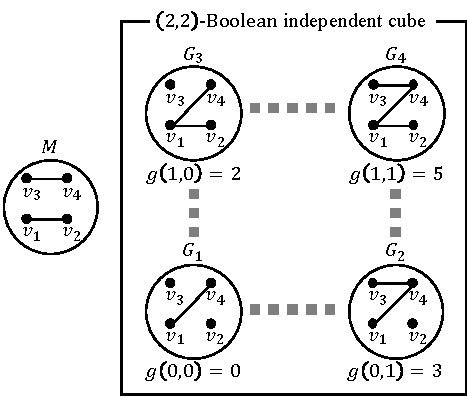
\includegraphics[width=0.88\linewidth]{fig/BoolCube.pdf}
  \vspace{-4mm}
  \caption{
    $(2,2)$-Boolean independent cube for $g$ corresponding to the $(4,2)$-independent cube for $f$ in Figure~\ref{fig:mono-cube}.
  }\label{fig:Bool-cube}
\end{figure}

Now, for $i \in [\kappa]$, define $\calS_i(x_i)$ for $x_i \in \{0,1\}$ by
% \[
\begin{align}
  \calS_i(x_i) = (\calR_{2i-1}(\bma_{2i-1} + x_i \bme_{2i}),
  \calR_{2i}(\bma_{2i} + x_i \bme_{2i-1})).
  \label{eq:S_i_R_2i_1}
\end{align}
% \]
In other words, $\calS_i(x_i)$ is simply the product of the outputs of users
$(v_{2i-1}, v_{2i})$, with $x_i$ indicating whether to add the edge in $M$ between them.

Assume that each $\calR_i$ is mutually independent and that $(\calR_1, \ldots, \calR_n)$ provides $\epsilon$-relationship DP in Definition~\ref{def:entire_edge_LDP}. 
Then by (\ref{eq:entire_edge_LDP}) and (\ref{eq:S_i_R_2i_1}), each $\calS_i$ provides $\epsilon$-DP and is mutually independent.
% Because the $\calR_i$ are mutually independent, we can conclude from
% Definition~\ref{def:entire_edge_LDP} that each $\calS_j(x)$ satisfies $\epsilon$-DP on the domain $\{0,1\}$. 

Define the estimator $\hat{g}$ by
\begin{align*}
  \hat{g}(x_1, \ldots, x_\kappa) &= \tilde{f}(\calS_1(x_1), \ldots,
  \calS_\kappa(x_\kappa)).
\end{align*}
Then by 
% We can apply 
Theorem~\ref{thm:lower-bound-dir}, 
% on $g$, $\hat{g}$, and the collection $\calS_1,\ldots, \calS_k$ to conclude that, 
for 
% $X \sim \{0,1\}^\kappa$,
$X=(x_1, \ldots, x_\kappa)$, 
\[
  \E_{X,\calS_1, \ldots, \calS_\kappa}[l_2^2(g(X), \hat{g}(X) )] \geq \Omega \left(
  \frac{e^{\varepsilon}}{(e^{\varepsilon}+1)^2} \kappa D^2 \right).
\]

Since 
% We are done by observing that 
there is a one-to-one correspondence between the ($n,D$)-independent cube $\calA$ 
and 
the ($\kappa,D$)-Boolean independent cube $\{0,1\}^\kappa$, we also have 
\[
  \E_{G,\calR_1, \ldots, \calR_n}[l_2^2(f(G), \hf(G))] \geq \Omega \left(
  \frac{e^{\varepsilon}}{(e^{\varepsilon}+1)^2} n D^2 \right),
\]
where $G$ is drawn uniformly from $\calA$, which proves Theorem~\ref{thm:lower-bound}. \qed
% and $\E_{\bmA, \calR_1, \ldots,
% \calR_n}[l_2^2(f(\bmA), \hf(\bmA))]$ is describing the same random process as
% $\E_{X, \calS_1, \ldots, \calS_k}[l_2^2(g(X), \hat{g}(X) )]$ with the variables
% renamed.

\subsection{Proof of
Theorem~\ref{thm:lower-bound-dir}}
\label{sub:proof_thm_lower-bound-dir}

Assume that $\calS_i : \{0,1\} \rightarrow \mathcal{Z}_i$.
For 
% $X \in \calX^n$, 
$X = (x_1, \ldots, x_\kappa) \in \{0,1\}^\kappa$, 
let $S(X) = (\calS_1(x_1), \cdots \calS_\kappa(x_\kappa))$ and
$Z = (z_1, \ldots, z_\kappa)$ with $z_i \in \mathcal{Z}_i$. 
We rewrite the quantity of interest as
\[
%\begin{align}
  \E_{X, S(X)}[l_2^2(g(X), \hg(X))] = \E_{X, S(X)}[(g(X)- \tilde{g}(S(X)))^2].
%  \label{eq:E_X_SX_l2}
\]
%\end{align}

% Using the law of total expectation, we condition on the event $S(X) = Z$:
By the law of total expectation, this quantity is the same as the expected value of the conditional expected value of $(g(X)- \tilde{g}(S(X)))^2$ given 
% we condition on the event 
$S(X) = Z$:
\begin{align}
  &\E_{X, S(X)}[(g(X)- \tilde{g}(S(X)))^2] \nonumber\\
  &= \E_{S(X)} \E_X[(g(X) - \tilde{g}(Z) )^2 | S(X)=Z].
  \label{eq:E_SX_X_g_tg}
\end{align}
% where for $Y \in \reals$
% $\E_{S(X)}[Y]$ represents the expectation of $Y$ over the randomness in $S$, and $\E_X[Y|S(X)=Z]$ represents the expectation of $Y$ over the randomness in selecting $X$ given $S(X)=Z$. 
Let $\mu_Z = \E_X[g(X)|S(X)=Z]$. 
Then the inner expectation in (\ref{eq:E_SX_X_g_tg}) can be written as follows:
% , with $\mu_Z = \E[g(X|S(X)=Z)]$,
\begin{align*}
  &\; \E_X[(g(X) - \tilde{g}(Z) )^2 | S(X)=Z] \\
  &= \E_X[( (g(X) - \mu_Z) + (\mu_Z - \tilde{g}(Z)) )^2 | S(X)=Z] \\
  &= \E_X[(g(X) - \mu_Z)^2 |S(X)=Z] \\
  &\hspace{3.5mm}+ 2(\mu_Z - \tilde{g}(Z))\E_X[(g(X) - \mu_Z)|S(X)=Z] \\
  &\hspace{3.5mm}+ (\mu_Z - \tilde{g}(Z))^2 \\
  &= \E_X[(g(X) - \mu_Z)^2 |S(X)=Z] + (\mu_Z - \tilde{g}(Z))^2 \\
  &= \V_X[g(X)|S(X)=Z] + (\mu_Z - \tilde{g}(Z))^2.
\end{align*}
Thus, it suffices to show that $\V_X[g(X)|S(X)=Z] \geq
\Omega\left(\frac{e^\epsilon}{(1+e^\epsilon)^2} \kappa D^2 \right)$.
For $B = (b_1, \ldots, b_\kappa) \in \{0,1\}^\kappa$, we have
\begin{align*}
  \Pr[X=B|S(X)=Z] = \frac{\Pr[X=B]\Pr[S(X)=Z|X=B]}{\Pr[S(X)=Z]}.
%   \Pr[X=B|S(X)=Z] &\propto \Pr[S(X)=Z|X=B]
\end{align*}
Since $\Pr[S(X)=Z]$ does not depend on $B$ and
$\Pr[X=B] = \frac{1}{2^\kappa}$, $\Pr[X=B|S(X)=Z]$ can also be expressed as 
\begin{align}
  \Pr[X=B|S(X)=Z] &\propto \Pr[S(X)=Z|X=B].
  \label{eq:X_B_SX_Z_propto}
\end{align}
% where the second line follows because $\Pr[S(X)=Z]$ does not depend on $B$ and
% $\Pr[X=B] = \frac{1}{2^\kappa}$.
% However, due to independence, 
Since $S_1, \ldots, S_\kappa$ are independently run, we have
% $\Pr[S(X)=Z|X=B]$ has the form
\begin{align*}
  \Pr[S(X)=Z|X=B] 
  &=
  %\;
  \Pr[\calS_1(b_1) = z_1, \ldots, \calS_\kappa(b_\kappa) = z_\kappa] \\
  &= \prod_{i=1}^\kappa \Pr[\calS_i(b_i)=z_i].
\end{align*}
Define 
%  \[
\begin{align*}
    % p_i = \frac{\Pr[\calS_i(x_i^{1})=z_i]}{\Pr[\calS_i(x_i^0)=z_i] +
    % \Pr[\calS_i(x_i^1)=z_i]}.
    p_i = \frac{\Pr[\calS_i(1)=z_i]}{\Pr[\calS_i(0)=z_i] +
    \Pr[\calS_i(1)=z_i]}.
%  \]
\end{align*}
Because each $\calS_i$ satisfies $\epsilon$-DP, we have $\frac{1}{1+e^{\epsilon}} \leq p_i \leq \frac{e^\epsilon}{1+e^\epsilon}$.
%The above equations tell us that
By (\ref{eq:X_B_SX_Z_propto}) and $\sum_{B \in \{0,1\}^\kappa} \Pr[X=B|S(X)=Z] = 1$, 
%$\Pr[X=B|S(X)=Z]$ can be expressed as 
we have
%  \[
\begin{align}
    \Pr[X=B|S(X)=Z] 
    %\propto 
    = 
    \prod_{i=1}^\kappa (p_i)^{b_i}(1-p_i)^{1-b_i}. %\\
%    &= \prod_{i=1}^\kappa \text{Bernoulli}(p_i),
%  \]
\label{eq:Pr_X_B_SX_Z_Bernoulli}
\end{align}
%where $\text{Bernoulli}(p_i)$ represents the Bernoulli distribution with parameter $p_i$.
This means that $\Pr[X=B|S(X)=Z]$ is distributed according to the independent product of $Bernoulli(p_i)$ for $i \in [\kappa]$.

Now, because 
%there is 
$g$ has 
a Boolean $(\kappa,D)$-independent cube, 
%for $g$, 
there are $C_1,
\ldots, C_\kappa \in \calS$ with $|C_i| \geq D$ such that
\begin{align*}
% g(X | S(X)=Z) &= g(0, \ldots, 0) + \sum_{i=1}^\kappa
% (x_i|S(X)=Z)C_i
g(X) &= g(0, \ldots, 0) + \sum_{i=1}^\kappa
x_iC_i.
\end{align*}
By (\ref{eq:Pr_X_B_SX_Z_Bernoulli}), 
% Because 
%$(x_i|S(X)=Z)$ 
$x_i$ 
is an independent draw from $Bernoulli(p_i)$ 
given $S(X)=Z$. 
Thus, the variance of 
%this quantity 
$g(X)$ given $S(X)=Z$ 
is
\begin{align*}
\V_X[g(X)|S(X)=Z] &= \sum_{i=1}^\kappa \V[x_i |S(X)=Z]C_i^2 \\
&\geq \sum_{i=1}^\kappa p_i(1-p_i) D^2 \\
&\geq \sum_{i=1}^\kappa \frac{e^\epsilon}{(1+e^\epsilon)^2} D^2 \\
&\geq \kappa \frac{e^\epsilon}{(1+e^\epsilon)^2} D^2.
\end{align*}
\qed
}
% \end{document}


%%%%%%%%%%%%%%%%%%%%%%%%%%%%%%%%%%%%%%%%%%%%%%%%%%%%%%%%%%%%%%%%%%%%%%%%%%%%%%%%
\end{document}
%%%%%%%%%%%%%%%%%%%%%%%%%%%%%%%%%%%%%%%%%%%%%%%%%%%%%%%%%%%%%%%%%%%%%%%%%%%%%%%%
